\chapter{Theoretical Framework}
The processing of sequential data constitutes a foundational pillar of modern Artificial Intelligence, particularly in Natural Language Processing (NLP) and, by extension, multimodal applications. For years, the state of the art in sequence modeling was defined by recurrent architectures \cite{rnn_sequence}, which, despite their successes, presented structural limitations regarding scalability and the retention of long-range dependencies \cite{analyticsvidhya}. The advent of the Transformer architecture marked a paradigm shift in the field, overcoming these bottlenecks through the introduction of the self-attention mechanism \cite{arxiv-attention}.\par
This chapter traces this crucial architectural evolution. The first section examines the theoretical foundations, operational mechanics, and inherent limitations of Recurrent Neural Networks (RNNs). Building upon this context, the subsequent sections delve into the Transformer architecture, detailing its core components and explaining how its highly parallelizable nature established the groundwork for modern Large Language Models (LLMs).

\section{Recurrent Neural Networks: Pre-Transformer State of the Art}
\label{chap:rnn}
\noindent
In recent years, the field of Artificial Intelligence has experienced an extraordinary evolution, driven by advances in deep learning, the increase in GPU computational power, and the availability of large-scale data. Until 2017, the majority of models for processing sequential data—such as text, biomedical signals, and time series—relied on \textbf{Recurrent Neural Networks (RNNs)} \cite{rnn_sequence, cs231n-rnn, quarkml-rnn-explained} and their variants, including Long Short-Term Memory (LSTM) networks, introduced by Hochreiter and Schmidhuber (1997), and Gated Recurrent Units (GRUs). These models represented the state of the art due to their ability to capture temporal dependencies and maintain memory of previous states, finding applications in speech recognition, machine translation, and natural language processing.

Although gating mechanisms mitigated the \textbf{vanishing/exploding gradient} problem \cite{quarkml-bptt}, recurrent architectures presented substantial limitations: \textbf{strictly sequential processing} hindered efficient parallelization, slowing down training on large datasets, and \textbf{modeling long-range dependencies} remained difficult, even when employing bidirectional variants or regularization strategies \cite{analyticsvidhya}. The breakthrough came in 2017 with the Transformer architecture, which replaced recurrence with \textbf{self-attention} mechanisms, allowing for the parallel processing of all positions in a sequence and more effective modeling of long-range relationships.

With the aim of contextualizing the advent of Transformers, this first section clearly introduces the basic operation of RNNs, highlighting their principles, strengths, and main limitations, thus laying the groundwork for comparison with subsequent architectures.

\subsection{RNN Architecture Overview}
\label{sub:recurrent_neural_networks}
\noindent
The distinctive element of \textbf{Recurrent Neural Networks (RNNs)} lies in their recurrent architecture, which allows information to propagate through feedback connections within the network \cite{cs231n-rnn, quarkml-rnn-explained, medium_math_rnn}. Unlike \textbf{Feedforward} neural networks, where data flows unidirectionally from input to output, RNNs introduce lateral connections that allow for the maintenance of temporal information \cite{medium_math_rnn}.

\begin{figure}[H]
\centering
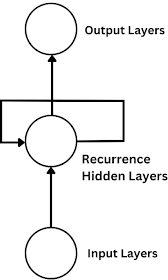
\includegraphics[width=0.25\linewidth]{img/rolled_rnn.png}
\caption{Basic scheme of a Recurrent Neural Network.}
\label{fig:rolled_rnn}
\end{figure}

Ideally, a Recurrent Neural Network can be visualized as a set of \textbf{Feed Forward Neural Networks (FFNNs)} where the hidden layers are connected one-to-one \cite{quarkml-rnn-explained}.
This structure can be understood by imagining a simple FFNN composed of:
\begin{itemize}
\item An input layer
\item Two hidden layers
\item An output layer
\end{itemize}
By connecting each hidden layer to every hidden layer of a second FFNN (constructed in the same way as the previous one) and repeating this operation $N$ times, a model like the one in the figure below is obtained \cite{quarkml-rnn-explained}.

\begin{figure}[H]
\centering
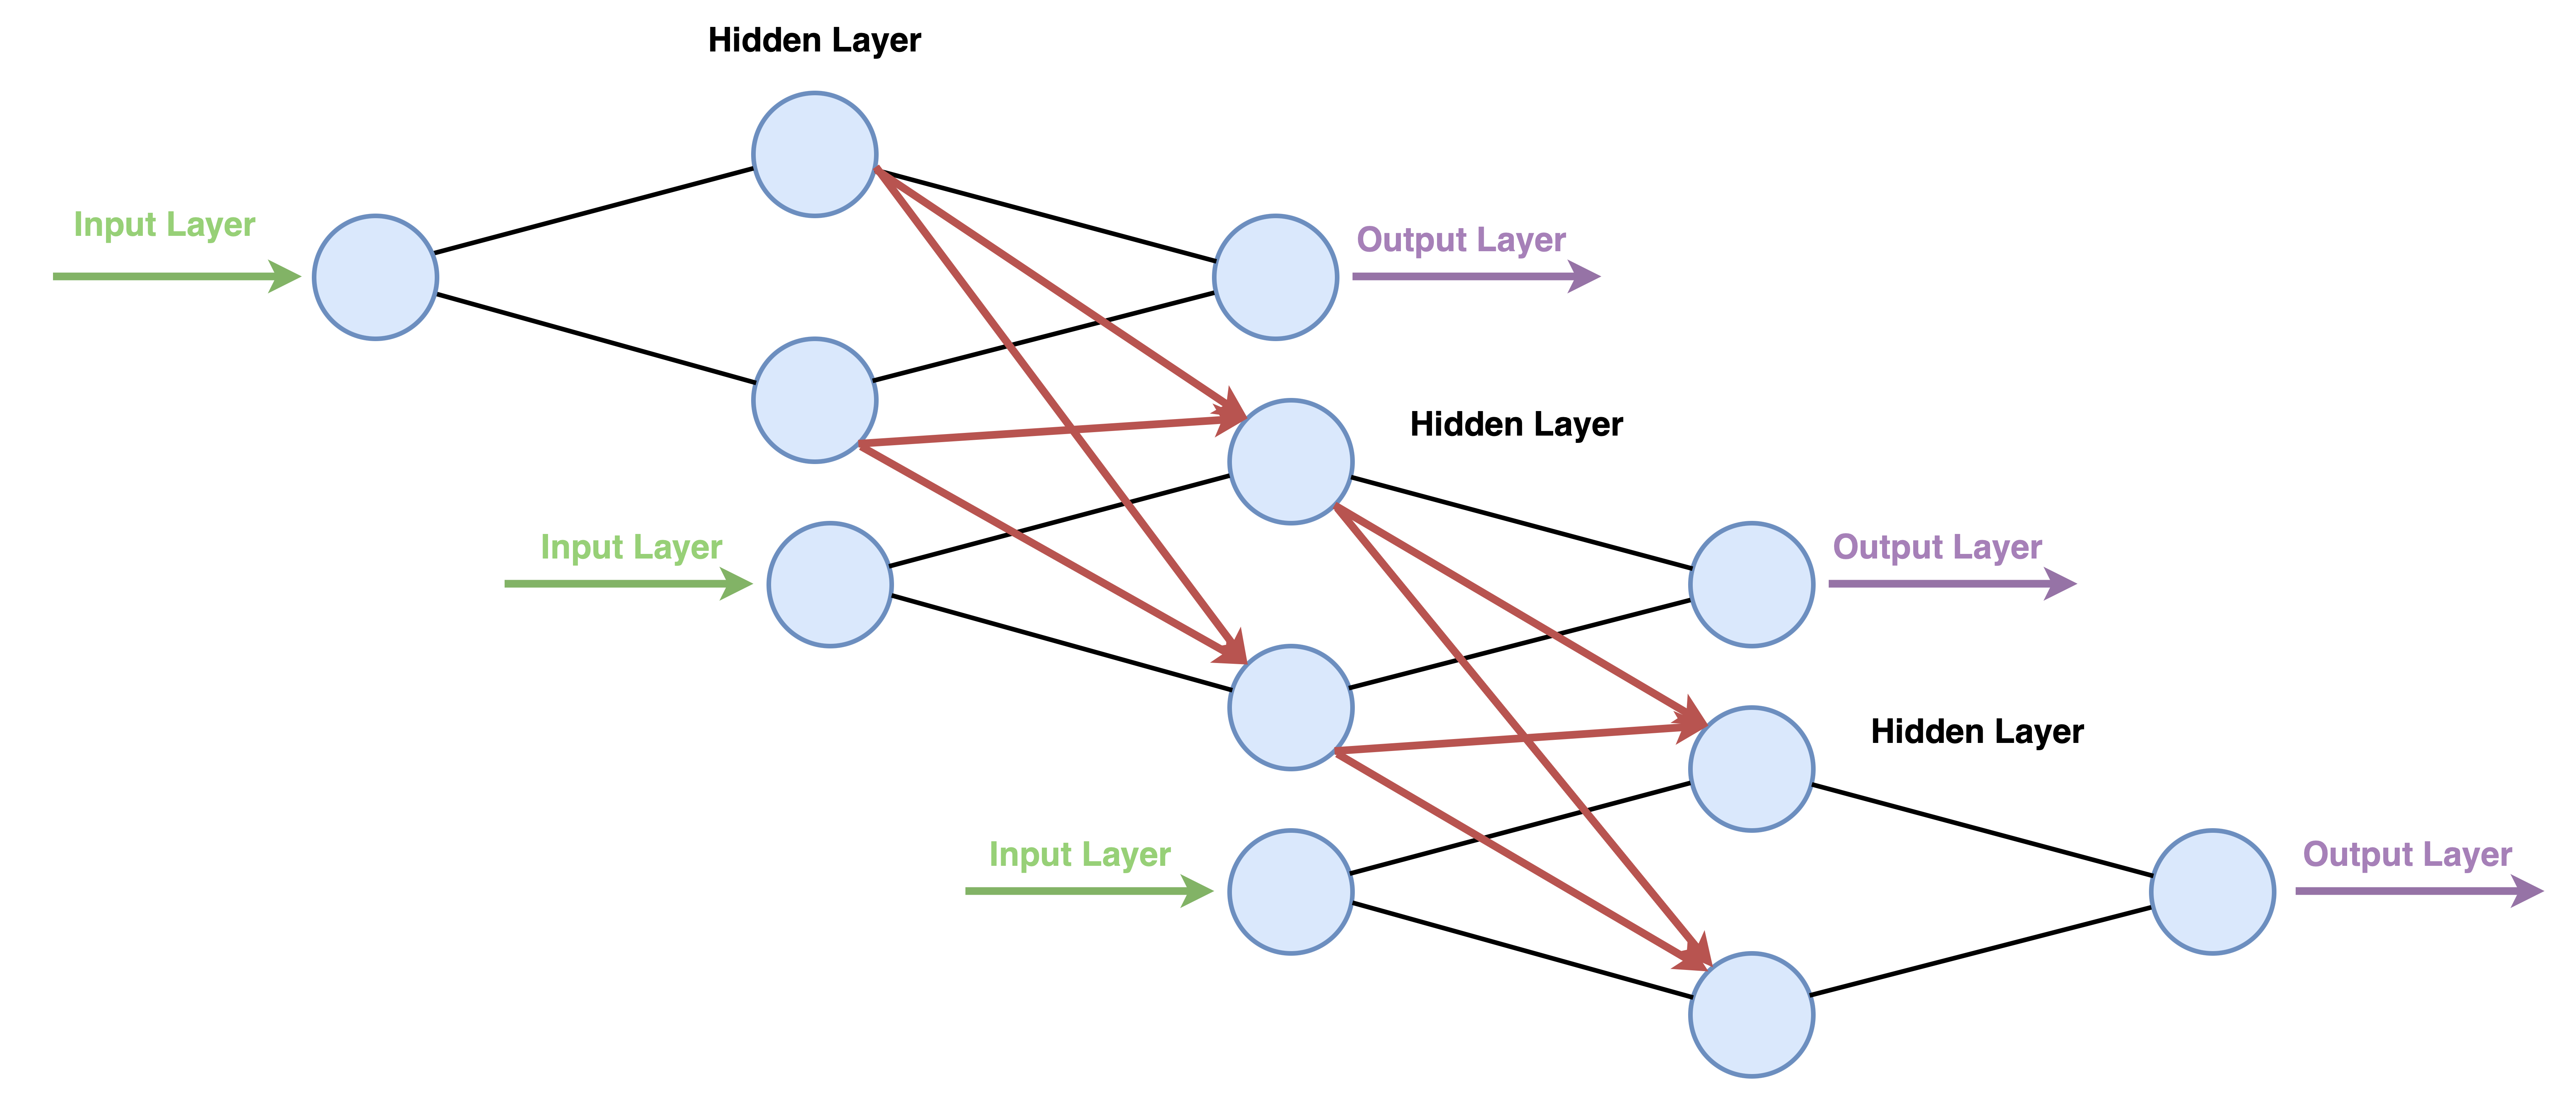
\includegraphics[width=1\linewidth]{img/rnn_hidden_layer2.png}
\caption{Visualization of an RNN with connected hidden layers \cite{quarkml-rnn-explained}. In this case, $N=3$.}
\label{fig:rnn_hidden_layer}
\end{figure}

From Figure \ref{fig:rnn_hidden_layer}, we can therefore understand how the network output depends on both the input from the input layer and the inputs arriving from the recurrent hidden layer.
Each of these individual FFNNs, to which the hidden layers are connected, is called a \textbf{time step} \cite{quarkml-rnn-explained}.

\begin{figure}[H]
\centering
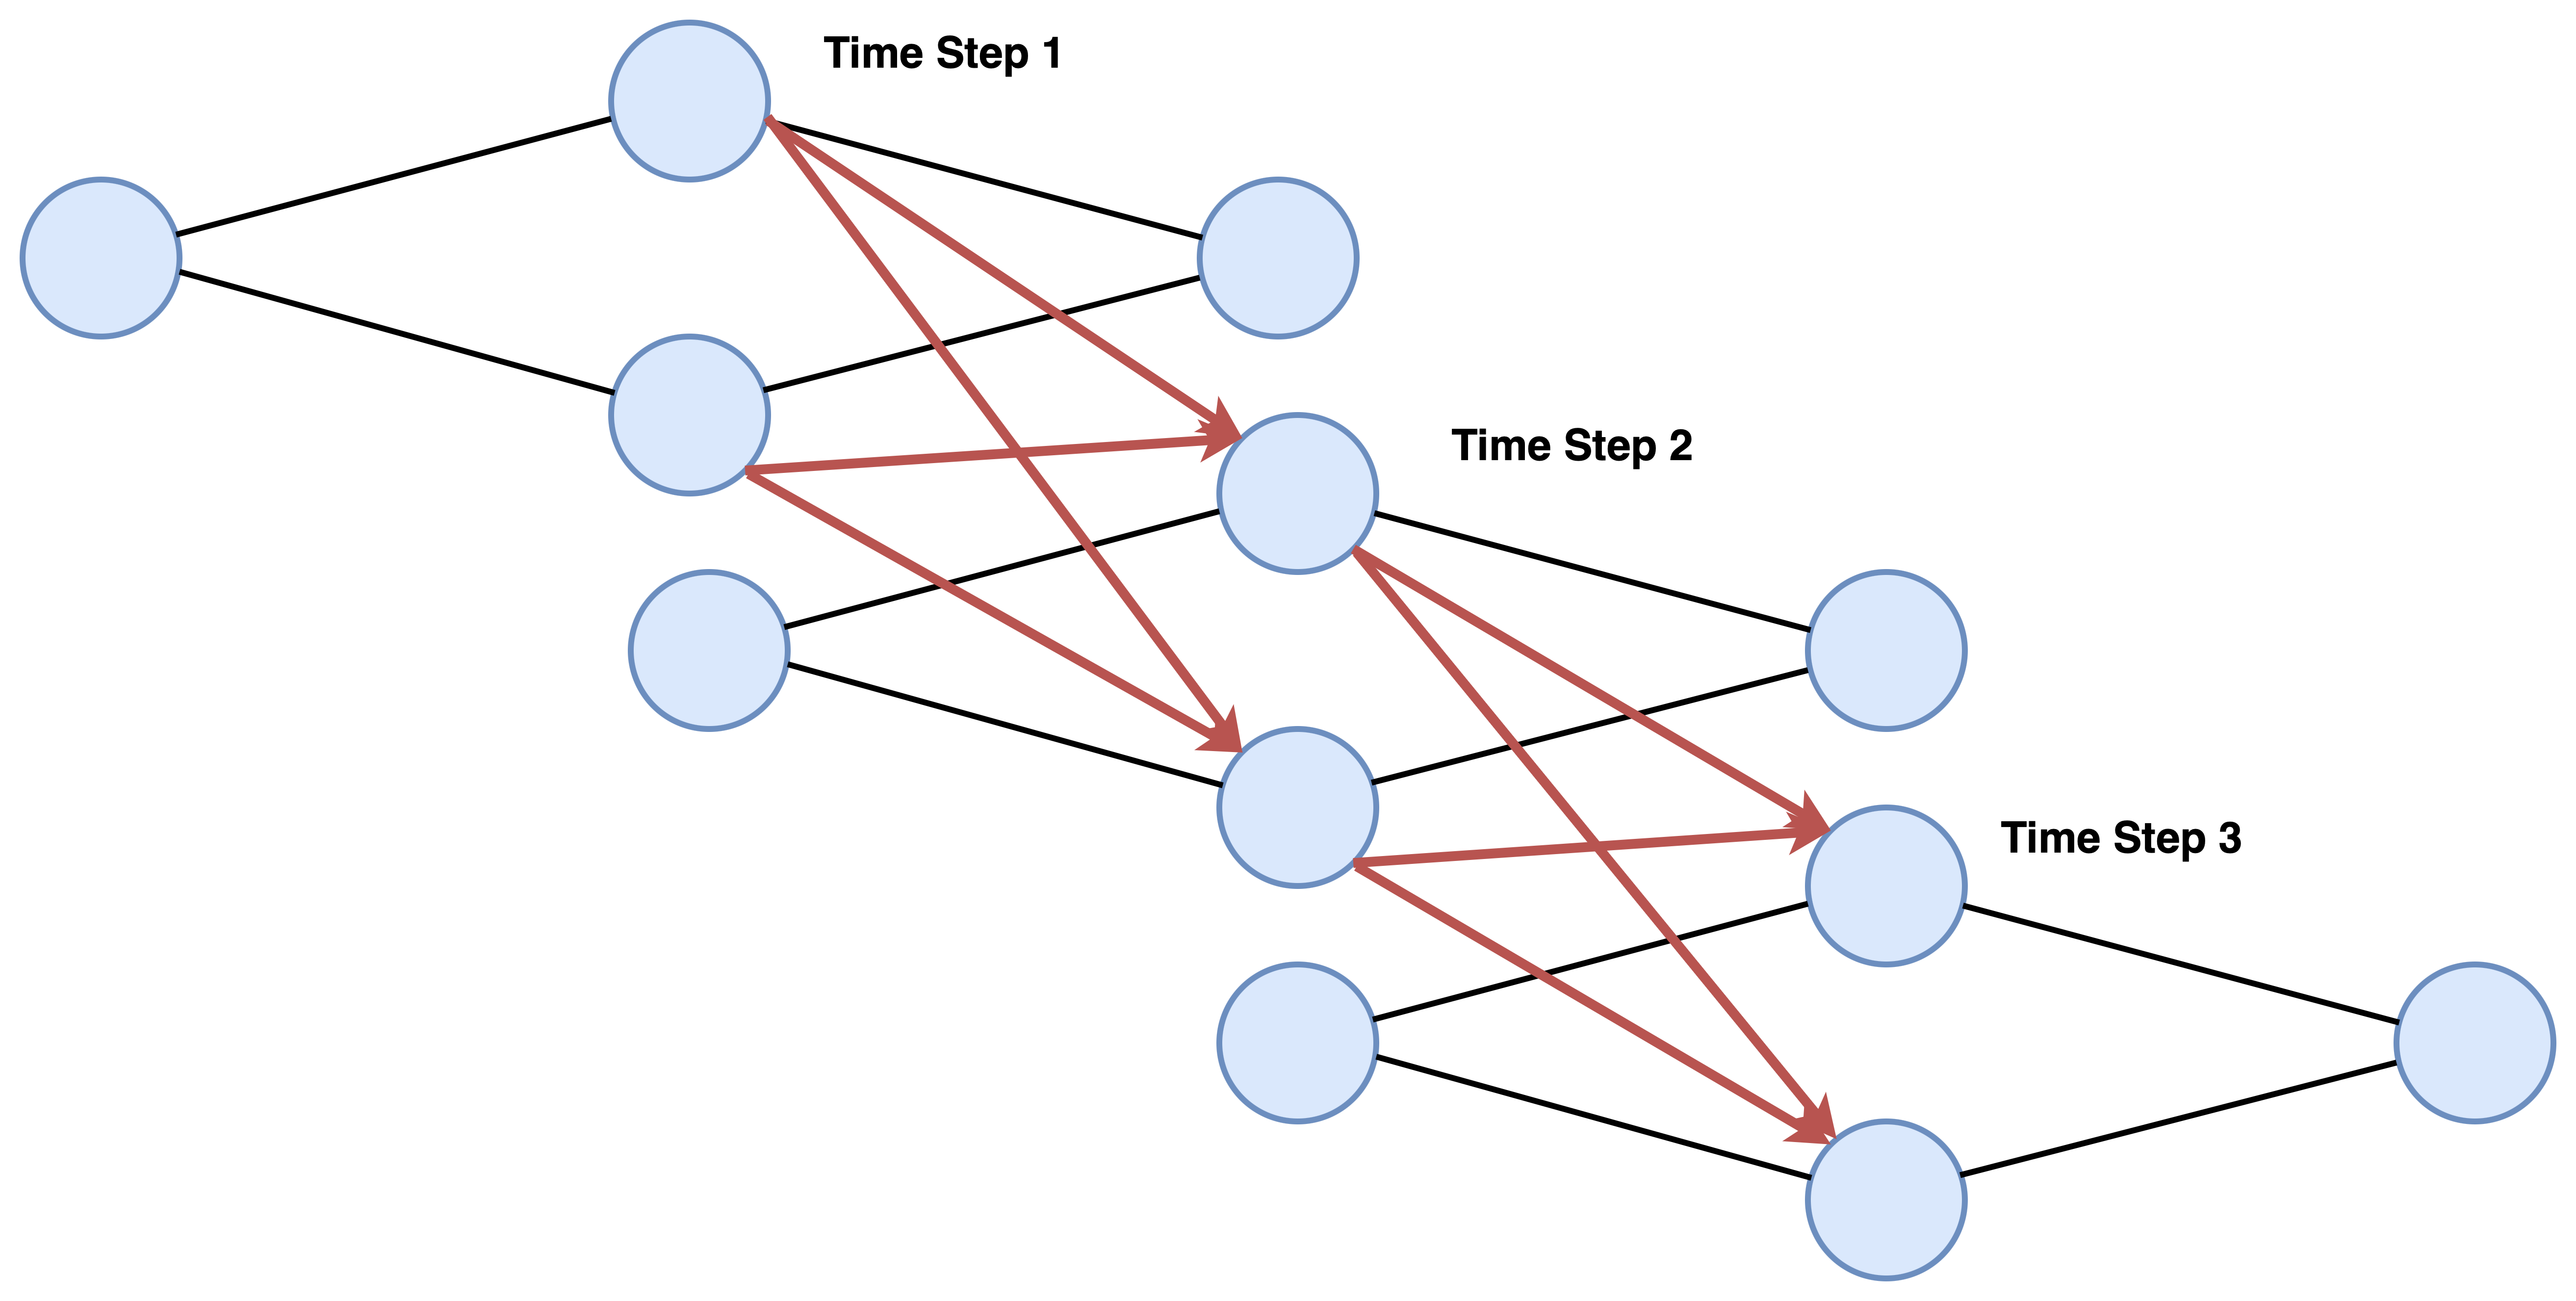
\includegraphics[width=0.8\linewidth]{img/rnn_hidden.png}
\caption{Visualization of an RNN time step \cite{quarkml-rnn-explained}.}
\end{figure}

A time step represents a discrete unit of time in the processing of a data sequence. More precisely, within an RNN, for an input sequence of length $T$, each time step $t$ (where $t$ ranges from $1$ to $T$) corresponds to a specific element of that sequence \cite{quarkml-rnn-explained}.

% spiegazione più concreta RNN.
\subsubsection{Introduction to the Structure of an RNN}
Structurally, an RNN is composed of four fundamental elements \cite{medium_math_rnn, quarkml-rnn-explained}:
\begin{itemize}
\item \textbf{Weights} ($W$): learned matrices that determine the importance of inputs and the previous state in generating the new state.
\item \textbf{Bias} ($b$): vectors added to each calculation to refine the network's response.
\item \textbf{Activation Function}: a \textbf{non-linear} function (e.g., $\tanh$, $\mathrm{ReLU}$, $\sigma$) used to compress the output to manageable values, introducing the capacity to learn complex relationships.
\item \textbf{Feedback Loop}: a recurrent connection that transmits part of the output of one step to the next, allowing the network to maintain a memory of previous information.
\end{itemize}

\begin{figure}[H]
\centering
 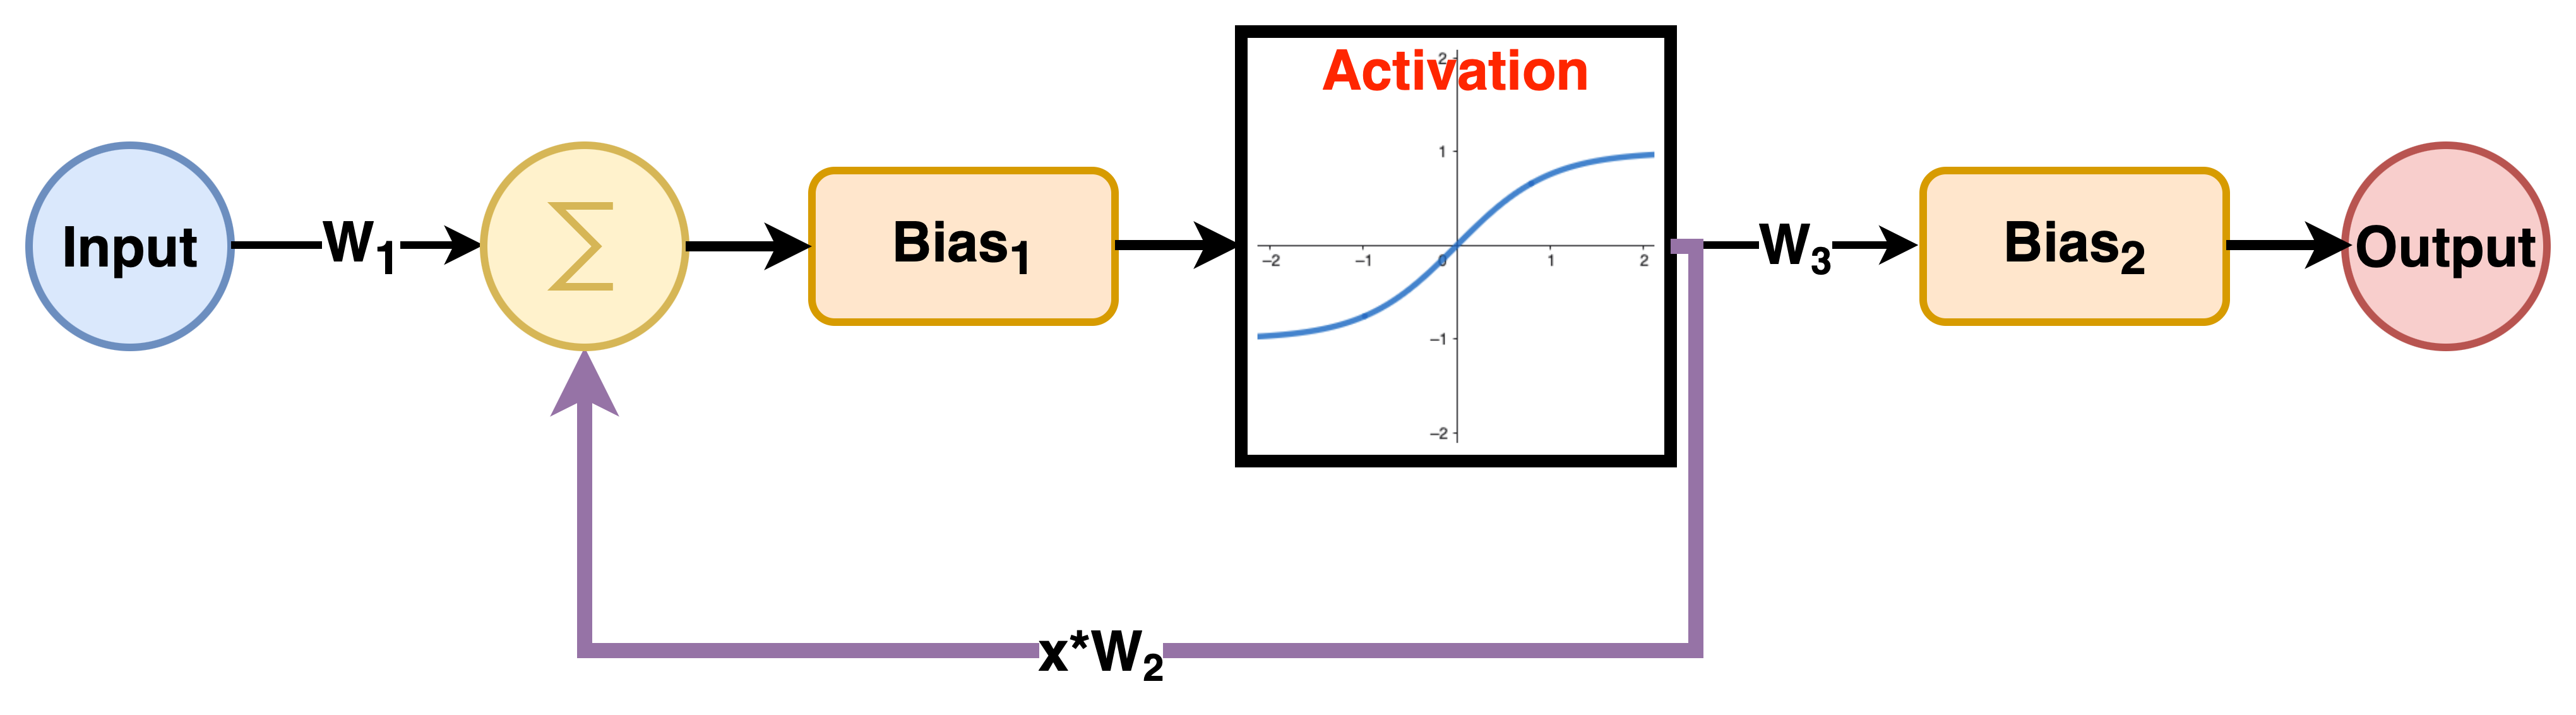
\includegraphics[width=0.8\linewidth]{img/rnn_rolled.png}
 \caption{Structure of an RNN.}
 \label{fig:rnn_rolled}
\end{figure}

The inputs of an RNN consist of a sequence $(input_1, input_2, \ldots, input_T)$, where each element $input_t$ is processed individually at each time step $t$. The \textbf{feedback loop} (highlighted in purple in Figures \ref{fig:rnn_rolled} and \ref{fig:rnn_unrolled}) allows the prediction related to input $input_t$ to be made by leveraging the state generated in the previous step (hidden state $h_{t-1}$) \cite{medium_math_rnn, quarkml-rnn-explained}.
To visualize the operation of an RNN more clearly, it is useful to consider its ``unrolled'' version, known as an \textbf{unrolled RNN}, as shown in Figure \ref{fig:rnn_unrolled} \cite{cs231n-rnn}.

\begin{figure}[H]
\centering
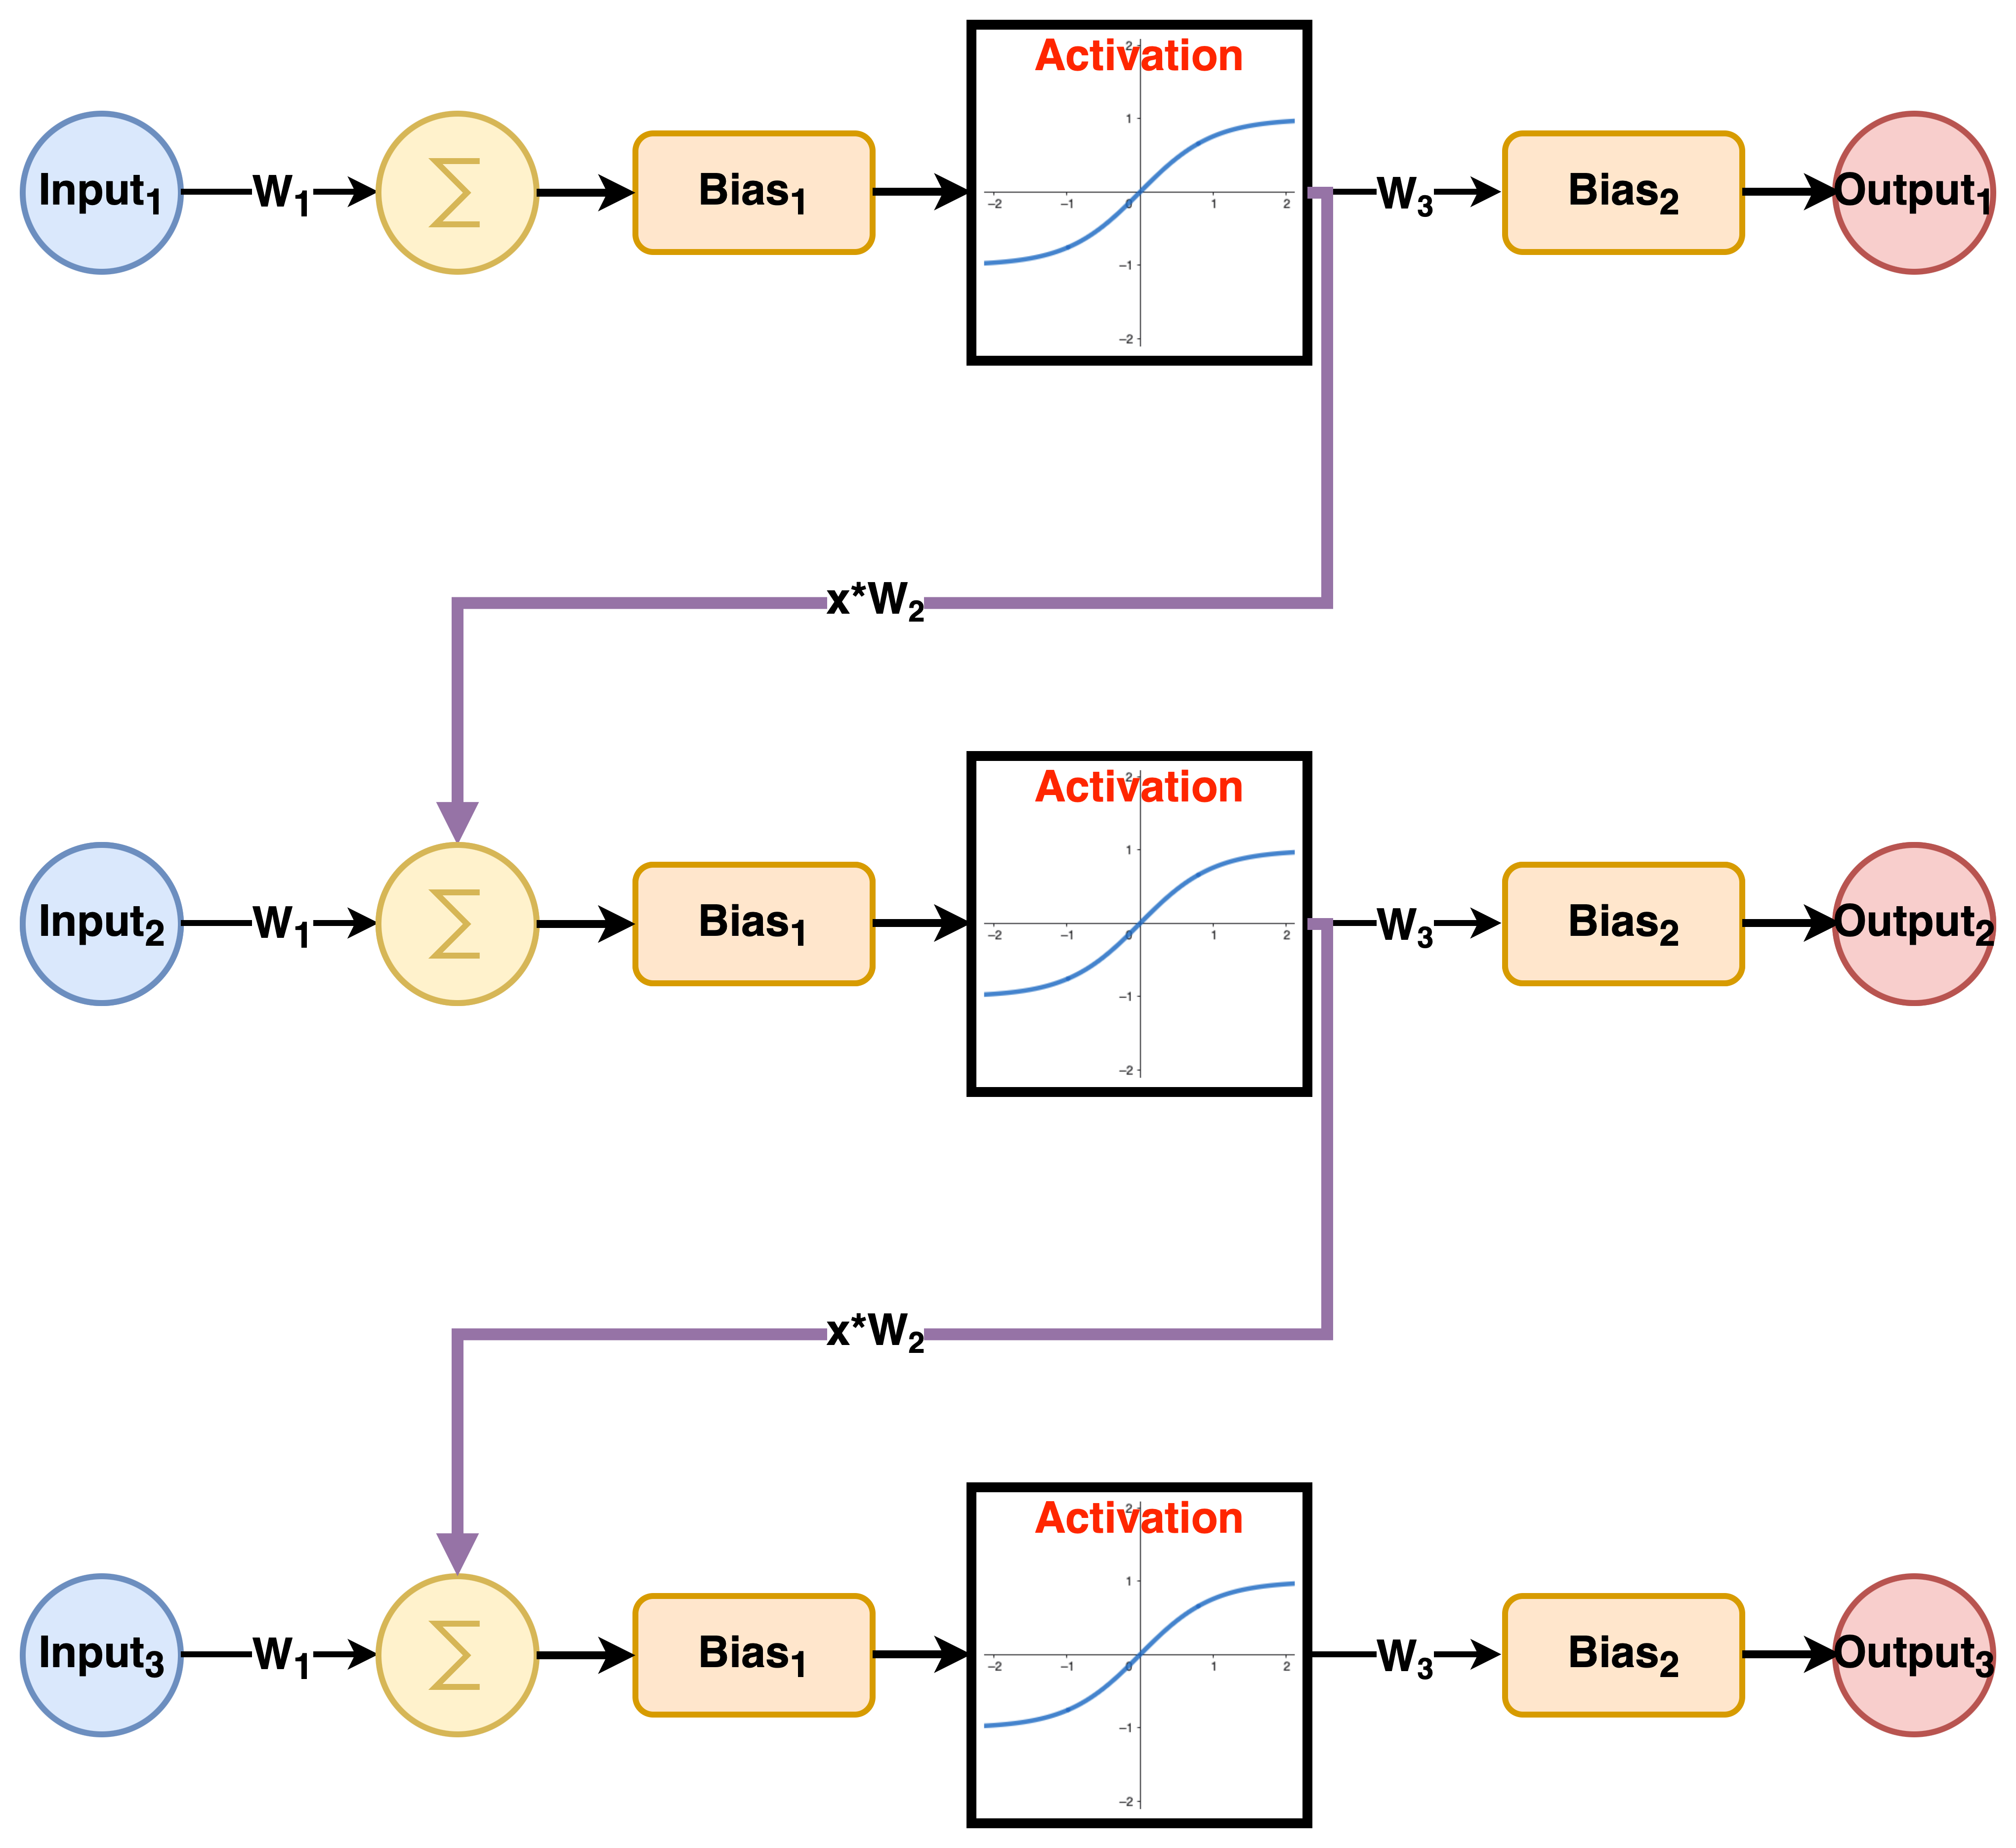
\includegraphics[width=0.8\linewidth]{img/rnn_unrolled.png}
\caption{Unrolled RNN with three states.}
\label{fig:rnn_unrolled}
\end{figure}

As can be observed, each feedback loop is added to the subsequent input (multiplied by $W_1$) \cite{medium_math_rnn}. This structure implies that the output of each single state $output_t$ is influenced not only by the current input $input_t$, but also by all previous inputs, since the state at step $t-1$ incorporates information accumulated from all preceding steps \cite{quarkml-rnn-explained}.
In a context where a decision or prediction based on the entire sequence is desired, $output_T$ is typically chosen precisely because it constitutes a complete representation that takes all previous states into account \cite{cs231n-rnn}.

\subsection{Mathematical Foundations of RNNs}
\noindent
Mathematically, an RNN can be represented through the recurrence formula \cite{cs231n-rnn, medium_math_rnn}:
\begin{equation}
h_t = f_W (h_{t-1}, x_t)
\end{equation}

where:
\begin{itemize}
    \item $h_t$ represents the hidden state at time step $t$
    \item $h_{t-1}$ represents the hidden state at time step $t-1$
    \item $x_t$ represents the input at time step $t$
    \item $f_W$ represents the state transition function with parameters $W$
\end{itemize}

The most elementary form of RNN, called \textbf{Vanilla RNN}, uses a single hidden state update formula \cite{cs231n-rnn}:
\begin{equation}
h_t = \tanh(W_{hh} h_{t-1} + W_{xh} x_t + b_h)
\label{formula:hidden_state_rnn}
\end{equation}


In matrix form:
\begin{equation}
\underbrace{
\begin{pmatrix} \bullet \\ \bullet \\ \bullet \\ \bullet \end{pmatrix}
}_{\mathbf{h}_t}
= \tanh \left(
\underbrace{
\begin{pmatrix}
\bullet & \bullet & \bullet & \bullet \\
\bullet & \bullet & \bullet & \bullet \\
\bullet & \bullet & \bullet & \bullet \\
\bullet & \bullet & \bullet & \bullet
\end{pmatrix}
}_{\mathbf{W}_{hh}}
\cdot
\underbrace{
\begin{pmatrix} \bullet \\ \bullet \\ \bullet \\ \bullet \end{pmatrix}
}_{\mathbf{h}_{t-1}}
+
\underbrace{
\begin{pmatrix}
\bullet & \bullet & \bullet \\
\bullet & \bullet & \bullet \\
\bullet & \bullet & \bullet \\
\bullet & \bullet & \bullet
\end{pmatrix}
}_{\mathbf{W}_{xh}}
\cdot
\underbrace{
\begin{pmatrix} \bullet \\ \bullet \\ \bullet \end{pmatrix}
}_{\mathbf{x}_t}
+
\underbrace{
\begin{pmatrix} \bullet \\ \bullet \\ \bullet \\ \bullet \end{pmatrix}
}_{\mathbf{b}_h}
\right)
\end{equation}

where:
\begin{itemize}
\item $W_{hh}$ represents the weight matrix for recurrent connections
\item $W_{xh}$ represents the weight matrix for input sequences
\item $b_h$ represents the hidden layer bias
\end{itemize}

Essentially, the sum of the projections of the weight matrices $W_{hh}$ and $W_{xh}$, for $h_{t-1}$ and $x_t$ respectively, is compressed through the $\tanh$ (hyperbolic tangent) function, which serves as the \textbf{\textit{activation function}} \cite{medium_math_rnn}. The result of this operation constitutes the hidden state $h_t$ of the RNN \cite{cs231n-rnn}.

Considering the most elementary case, it is possible to base predictions directly on $h_t$ by simply performing a final transformation \cite{medium_math_rnn, quarkml-rnn-explained}:
\begin{equation}
o_t = W_{ho}h_t + b_o
\end{equation}


In matrix form:
\begin{equation}
\underbrace{
\begin{pmatrix} \bullet \\ \bullet \end{pmatrix}
}_{\mathbf{o}_t}
=
\underbrace{
\begin{pmatrix}
\bullet & \bullet & \bullet & \bullet \\
\bullet & \bullet & \bullet & \bullet
\end{pmatrix}
}_{\mathbf{W}_{ho}}
\cdot
\underbrace{
\begin{pmatrix} \bullet \\ \bullet \\ \bullet \\ \bullet \end{pmatrix}
}_{\mathbf{h}_t}
+
\underbrace{
\begin{pmatrix} \bullet \\ \bullet \end{pmatrix}
}_{\mathbf{b}_o}
\end{equation}

where:
\begin{itemize}
\item $W_{ho}$ represents a weight matrix (hidden-to-output)
\item $b_o$ represents the output bias
\item $o_t$ represents the vector of output logits from the model at time $t$
\end{itemize}

The weight matrices $W_{hh}$, $W_{xh}$, and $W_{ho}$ are learned via \textbf{Backpropagation Through Time} (BPTT) \cite{quarkml-bptt}, an extension of the traditional backpropagation algorithm adapted for training Recurrent Neural Networks.

\subsubsection{Practical Case Study: Character-Level Modeling}
To provide a more practical understanding of how an RNN operates, we illustrate its functioning step-by-step as a Character-Level Language Model \cite{cs231n-rnn}. In this example (for simplicity), the bias vectors are set with all elements to zero: $b_h = [0,0,...,0]^T,b_o = [0,0,...,0]^T$. The objective is to show how an RNN, given a sequence of characters, predicts the next character. At each time step, the network must provide a probability distribution over the vocabulary characters, indicating which character should come next in the sequence \cite{cs231n-rnn, quarkml-rnn-explained}.

The computation process develops in the following phases:
\begin{enumerate}
\item \textbf{Vocabulary Construction:} A vocabulary containing all unique characters present in the training corpus is defined \cite{cs231n-rnn}.

\item \textbf{Input Representation:} Each character in the vocabulary is transformed into a numerical representation. A common technique is one-hot encoding, where each character corresponds to a binary vector with a single element equal to 1 and all others to 0. The vector dimension is equal to the vocabulary size \cite{quarkml-rnn-explained}.

\item \textbf{Computation Process:} At each time step $t$, the RNN receives the one-hot vector of the current character $x_t$ and the hidden state of the previous step $h_{t-1}$ as input. Its task is to produce an output $y_t$ representing a probability distribution over the next character $x_{t+1}$ \cite{cs231n-rnn, medium_math_rnn}.

\end{enumerate}

We use the input sequence \texttt{hello} as an example; the RNN's task will therefore be to:
\begin{itemize}
\item Given \texttt{"h"} predict \texttt{"e"}
\item Given \texttt{"he"} predict \texttt{"l"}
\item Given \texttt{"hel"} predict \texttt{"l"}
\item Given \texttt{"hell"} predict \texttt{"o"}
\end{itemize}
Note that, in this case, the training corpus consists solely of the string \texttt{hello} with a vocabulary $V=\{\texttt{``h''}, \texttt{``e''}, \texttt{``l''}, \texttt{``o''}\}$ of four characters.

Each character in the vocabulary is represented using \textbf{one-hot} encoding, i.e., through vectors in which only one element is \textit{\textbf{1}} and all others are \textit{\textbf{0}}. The length of each vector is equal to the vocabulary cardinality, in this case $|V|=4$:
\[
\begin{bmatrix} 1 \\ 0 \\ 0 \\ 0 \end{bmatrix} = \text{``h''} \quad
\begin{bmatrix} 0 \\ 1 \\ 0 \\ 0 \end{bmatrix} = \text{``e''} \quad
\begin{bmatrix} 0 \\ 0 \\ 1 \\ 0 \end{bmatrix} = \text{``l''} \quad
\begin{bmatrix} 0 \\ 0 \\ 0 \\ 1 \end{bmatrix} = \text{``o''}
\]

The core of the process is the recursive update of the hidden state through \\ $h_t = \tanh(W_{hh} h_{t-1} + W_{xh} x_t)$ which, setting the weight matrices $W$ to \textit{random} values, develops as:

\begin{align}
\begin{bmatrix} 0.3 \\ -0.1 \\ 0.9 \end{bmatrix} &= f_W \left( W_{hh} \begin{bmatrix} 0 \\ 0 \\ 0 \end{bmatrix} + W_{xh} \begin{bmatrix} 1 \\ 0 \\ 0 \\ 0 \end{bmatrix} \right) \tag{$h_1$} \\[1.5em]
\begin{bmatrix} 1.0 \\ 0.3 \\ 0.1 \end{bmatrix} &= f_W \left( W_{hh} \begin{bmatrix} 0.3 \\ -0.1 \\ 0.9 \end{bmatrix} + W_{xh} \begin{bmatrix} 0 \\ 1 \\ 0 \\ 0 \end{bmatrix} \right) \tag{$h_2$} \\[1.5em]
\begin{bmatrix} 0.1 \\ -0.5 \\ -0.3 \end{bmatrix} &= f_W \left( W_{hh} \begin{bmatrix} 1.0 \\ 0.3 \\ 0.1 \end{bmatrix} + W_{xh} \begin{bmatrix} 0 \\ 0 \\ 1 \\ 0 \end{bmatrix} \right) \tag{$h_3$} \\[1.5em]
\begin{bmatrix} -0.3 \\ 0.9 \\ 0.7 \end{bmatrix} &= f_W \left( W_{hh} \begin{bmatrix} 0.1 \\ -0.5 \\ -0.3 \end{bmatrix} + W_{xh} \begin{bmatrix} 0 \\ 0 \\ 1 \\ 0 \end{bmatrix} \right) \tag{$h_4$}
\end{align}

The output is then calculated iteratively, in the form of scores (\textit{logits}) at time $t$, for each single $h_t$ using $y_t = W_{ho}h_t$:

\begin{figure}[H]
\centering
\begin{tikzpicture}[
node distance=1.5cm and 1cm,
input/.style={rectangle, draw, fill=red!15, minimum height=1.6cm, minimum width=1cm, align=center, font=\small},
hidden/.style={rectangle, draw, fill=green!15, minimum height=1.2cm, minimum width=1cm, align=center, font=\small},
output/.style={rectangle, draw, fill=blue!15, minimum height=1.6cm, minimum width=1cm, align=center, font=\small},
io_char/.style={align=center, font=\small},
layer_label/.style={text width=2.5cm, align=right, font=\small\bfseries},
weight_label/.style={midway, fill=white, inner sep=1pt, font=\tiny},
]

% Layer Labels
\node[layer_label, text=red!60!black] at (-2, -2.5) {input layer};
\node[layer_label, text=green!50!black] at (-2, 0) {hidden layer};
\node[layer_label, text=blue!60!black] at (-2, 2.5) {output layer};

% Time Step 1 (h) -> e
\node[input] (x1) at (0, -2.5) {$1$\\$0$\\$0$\\$0$};
\node[io_char] (char_x1) [below=0.1cm of x1] {``h''};
\node[hidden] (h1) at (0, 0) {$0.3$\\$-0.1$\\$0.9$};
\node[output] (y1) at (0, 2.5) {\color{red} $1.0$\\ \color{green!50!black} $2.2$\\ \color{red} $-3.0$\\ \color{red}$4.1$};
\node[io_char] (char_y1) [above=0.1cm of y1] {``e''};

% Time Step 2 (e) -> l
\node[input] (x2) [right=2cm of x1] {$0$\\$1$\\$0$\\$0$};
\node[io_char] (char_x2) [below=0.1cm of x2] {``e''};
\node[hidden] (h2) [right=2cm of h1] {$1.0$\\$0.3$\\$0.1$};
\node[output] (y2) [right=2cm of y1] {\color{red} $0.5$\\ \color{red} $0.3$\\ \color{green!50!black} $-1.0$\\ \color{red} $1.2$};
\node[io_char] (char_y2) [above=0.1cm of y2] {``l''};

% Time Step 3 (l) -> l
\node[input] (x3) [right=2.05cm of x2] {$0$\\$0$\\$1$\\$0$};
\node[io_char] (char_x3) [below=0.1cm of x3] {``l''};
\node[hidden] (h3) [right=2cm of h2] {$0.1$\\$-0.5$\\$-0.3$};
\node[output] (y3) [right=2cm of y2] {\color{red} $0.1$\\\color{red} $0.5$\\ \color{green!50!black} $1.9$\\ \color{red} $-1.1$};
\node[io_char] (char_y3) [above=0.1cm of y3] {``l''};

% Time Step 4 (l) -> o
\node[input] (x4) [right=2.05cm of x3] {$0$\\$0$\\$1$\\$0$};
\node[io_char] (char_x4) [below=0.1cm of x4] {``l''}; % Note: image has 'l' as input for 'o'
\node[hidden] (h4) [right=2cm of h3] {$-0.3$\\$0.9$\\$0.7$};
\node[output] (y4) [right=2cm of y3] {\color{red} $0.2$\\ \color{red} $-1.5$\\ \color{red} $-0.1$\\ \color{green!50!black} $2.2$};
\node[io_char] (char_y4) [above=0.1cm of y4] {``o''};

% Arrows and Weight Labels
% Input to Hidden
\draw[-{Stealth[length=2mm]}, red!60!black] (x1) -- (h1) node[weight_label, pos=0.8, right=1mm] {$W_{xh}$};
\draw[-{Stealth[length=2mm]}, red!60!black] (x2) -- (h2);
\draw[-{Stealth[length=2mm]}, red!60!black] (x3) -- (h3);
\draw[-{Stealth[length=2mm]}, red!60!black] (x4) -- (h4);

% Hidden to Hidden
\draw[-{Stealth[length=2mm]}, green!50!black] (h1) -- (h2) node[weight_label, pos=0.6, above=1mm] {$W_{hh}$};
\draw[-{Stealth[length=2mm]}, green!50!black] (h2) -- (h3);
\draw[-{Stealth[length=2mm]}, green!50!black] (h3) -- (h4);

% Hidden to Output
\draw[-{Stealth[length=2mm]}, blue!60!black] (h1) -- (y1) node[weight_label, pos=0.8, right=1mm] {$W_{hy}$};
\draw[-{Stealth[length=2mm]}, blue!60!black] (h2) -- (y2);
\draw[-{Stealth[length=2mm]}, blue!60!black] (h3) -- (y3);
\draw[-{Stealth[length=2mm]}, blue!60!black] (h4) -- (y4);

\end{tikzpicture}
\caption{Calculation of \textit{logits} by processing the sequence \texttt{``hell''} for each $h_t$.}
\end{figure}

The acquired scores are then normalized using a function, typically \textbf{softmax} $\sigma(o_t)$, to obtain a probability distribution. 
\[
\begin{array}{c}
\text{\textit{Output layer}} \\
\begin{bmatrix} 1.0 \\ 2.3 \\ -3.0 \\ 4.1 \end{bmatrix}
\end{array}
\quad \rightarrow \quad
\begin{array}{c}
\text{\textbf{softmax}} \\
\sigma(o_t) = \displaystyle\frac{e^{o_{i}}}{\sum_{j=1}^{|V|} e^{o_{j}}} \quad i = 1,\dots,|V|
\end{array}
\quad \rightarrow \quad
\begin{array}{c}
\text{\textit{Probabilities}} \\
\begin{bmatrix} 0.03719 \\ 0.13648 \\ 0.00068 \\ 0.82565 \end{bmatrix}
\end{array}
\]

During training, the error between the predicted distribution and the target character (represented as a one-hot vector) is calculated via a cost function such as \textbf{cross-entropy} \cite{cs231n-rnn, quarkml-bptt}. This error is then minimized by updating the network weights through \textbf{Backpropagation Through Time} \cite{quarkml-bptt, cs231n-rnn}.

This mechanism allows the network not only to associate an input with an output but to do so in a context-dependent manner \cite{cs231n-rnn}. \footnote{Naturally, with random weights, the prediction is likely wrong. The next section explains how BPTT iteratively adjusts these matrices to minimize the error shown in the example \cite{quarkml-bptt}.}% Ad esempio, nel predire il carattere dopo la prima \texttt{"l"} di \texttt{"hello"}, la rete deve produrre un'altra \texttt{"l"}, mentre dopo la seconda deve produrre una \texttt{"o"}. Questa distinzione è possibile solo grazie all'informazione contestuale accumulata nell'hidden state.
\bigskip

\subsection{Backpropagation Through Time}
The goal of BPTT is to minimize the total loss of an output sequence (with respect to the correct output sequence) by backpropagating the error from the outputs to the respective hidden states and, through recurrence, from future states to past ones \cite{quarkml-bptt}. The shared nature of the weights implies that each parameter receives the sum of contributions from all time steps in which it is used \cite{quarkml-bptt}.

To apply backpropagation, it is necessary to transform the cyclic nature of the RNN into a \textbf{FeedForward} (thus acyclic) structure; the resulting RNN is called an Unrolled RNN \cite{quarkml-bptt, cs231n-rnn}.

To obtain an Unrolled RNN starting from a classic RNN \cite{quarkml-rnn-explained}:
\begin{itemize}
\item The RNN is "unrolled" along the time sequence.
\item Each time step $t$ becomes a layer of the network.
\item Weights are shared across all temporal layers.
\end{itemize}

An unrolled RNN can be visualized in Figure \ref{fig:rnn}; the state \textit{"state 0"} represents the initial state of the RNN. The initial state is typically set as a vector of all zeros \cite{cs231n-rnn}.

\begin{figure}[H]
\centering
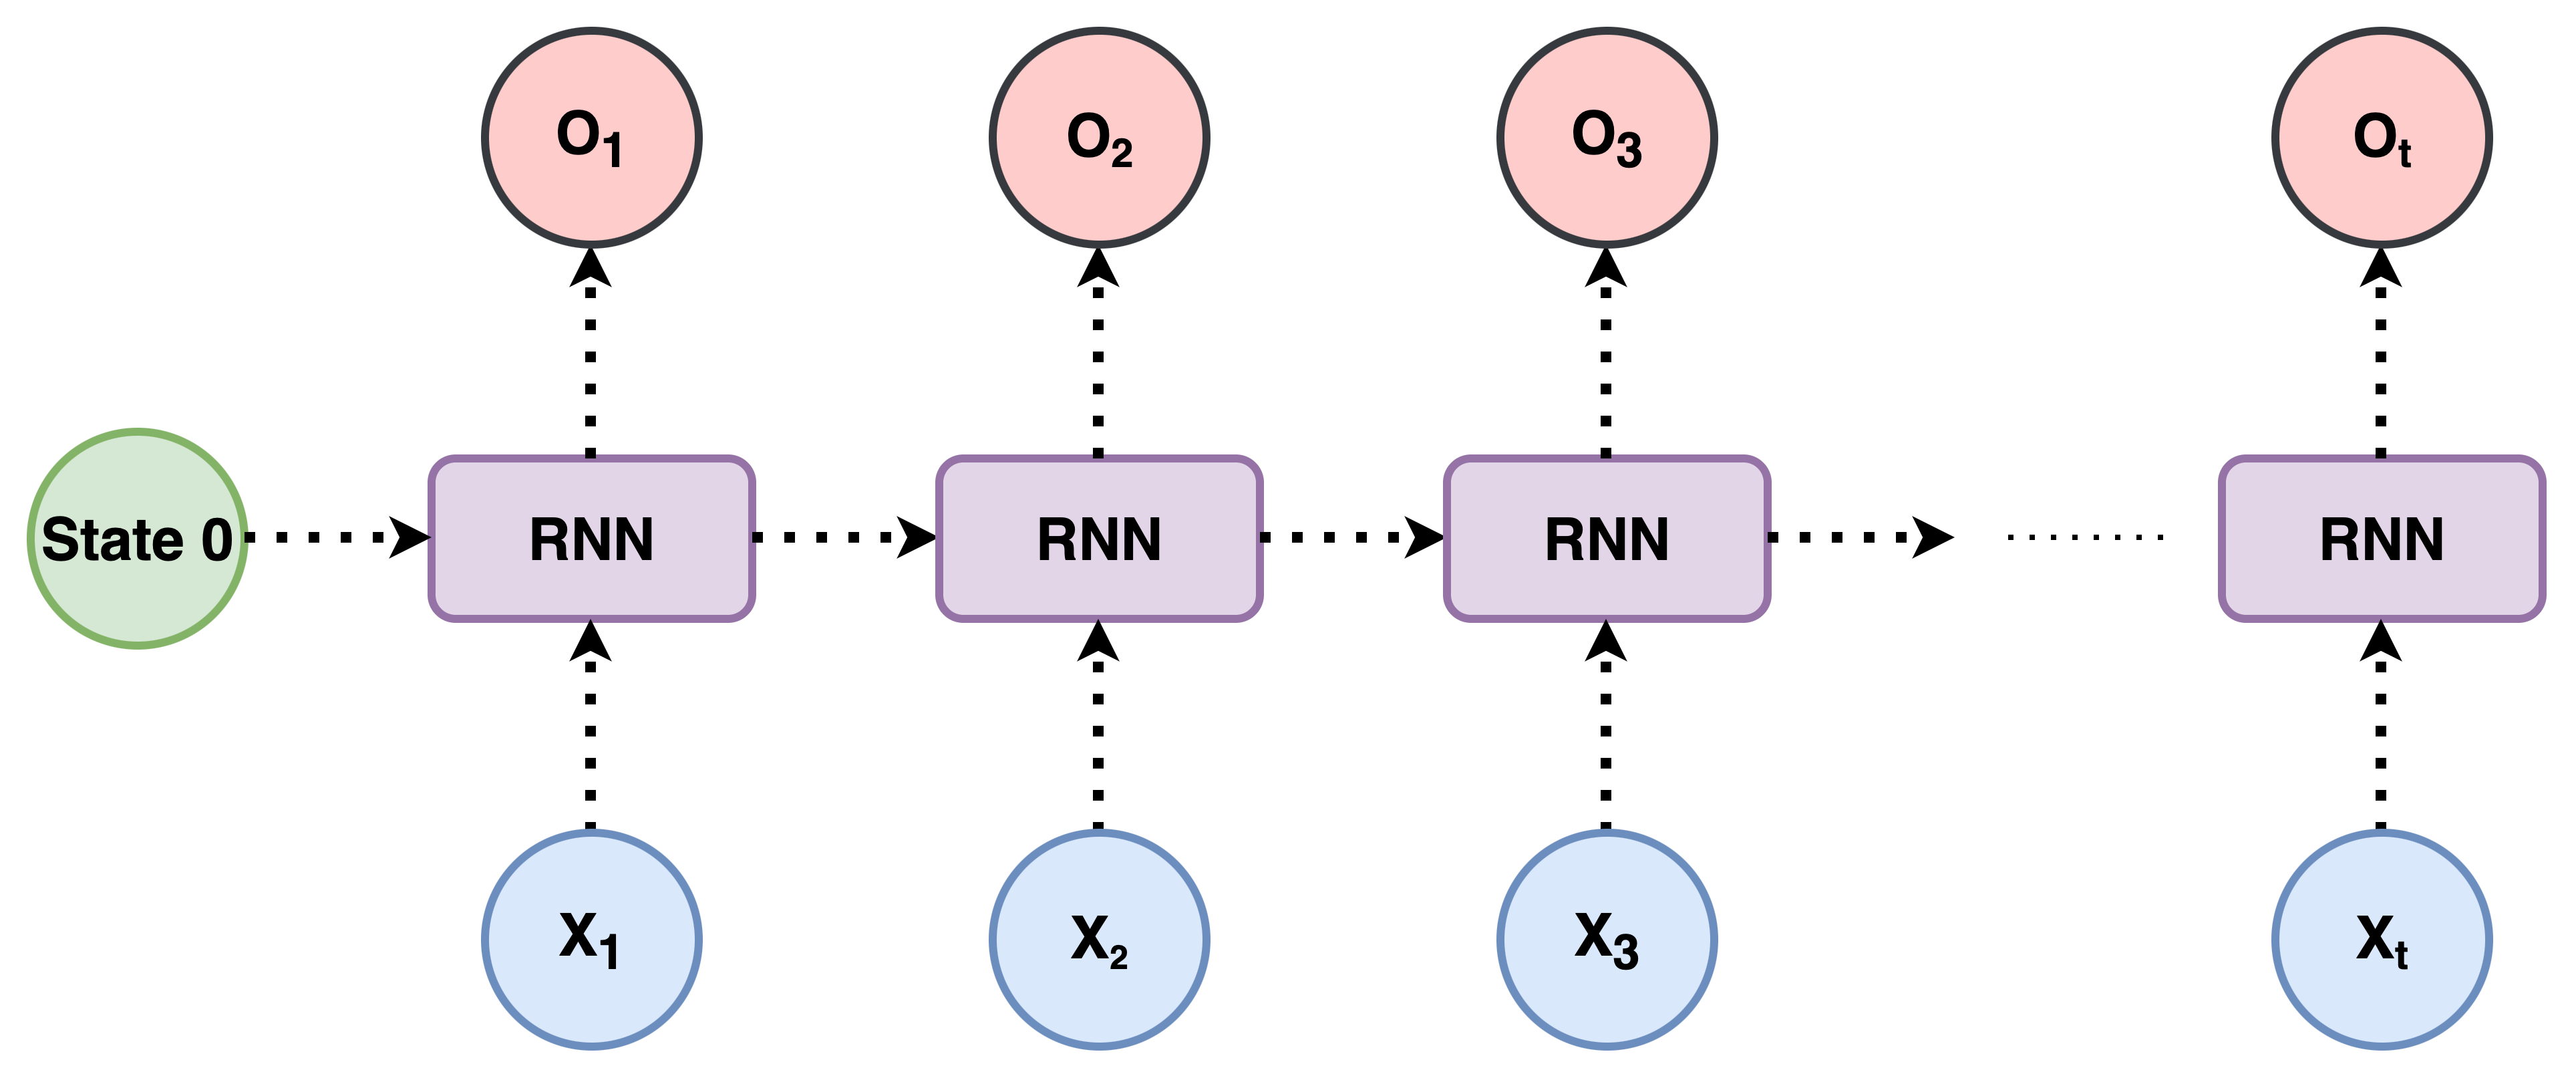
\includegraphics[width=0.8\linewidth]{img/rnn_o.png}
\caption{Graphical representation of an Unrolled Vanilla RNN.}
\label{fig:rnn}
\end{figure}

Considering a vanilla RNN with activation function $\phi$, we define:
$$
h_t = \phi(W_{xh} X_t + W_{hh} h_{t-1} + b_h), \quad o_t=W_{ho}h_t+b_o, \quad \hat{y}=\text{softmax}(o_t)
$$
where:
\begin{itemize}
\item $\phi$ represents the activation function
\item $\hat{y}_t$ represents the predicted probability vector at time $t$
\end{itemize}

The steps of the BPTT algorithm are as follows \cite{quarkml-bptt}:

\paragraph{Forward Pass} For each time step $t$ from $1$ to $T$, the following quantities are calculated \cite{medium_math_rnn, quarkml-bptt}:

\begin{itemize}
\item Hidden state $\rightarrow h_t = \phi(W_{xh} X_t + W_{hh} h_{t-1} + b_h)$
\item Output logits $\rightarrow o_t=W_{ho}h_t+b_o$ % Nota: Ho corretto h_o in h_t come discusso prima, se preferisci l'originale rimetti h_o
\item Predicted probabilities $\hat{y}=\text{softmax}(o_t)$
\end{itemize}
The aggregate loss $L$, i.e., the sum of the loss functions calculated at each individual time step of the sequence, is given by \cite{quarkml-bptt}:
\begin{equation}
L =\sum^T_{t=1} \ell_t(o_t, y_t)
\end{equation}
where:
\begin{itemize}
\item $\ell_t$ represents the loss function calculated at time step $t$
\item $y_t$ represents the correct result (ground truth)
\end{itemize}

In this case, we set $L=\text{MSE}$, \footnote{Although Cross-Entropy is the standard loss function for multi-class classification tasks, Mean Squared Error (MSE) is adopted here to simplify the mathematical derivation of the gradients \cite{quarkml-bptt}.} yielding:
\begin{equation}
L = \frac{1}{T} \sum^T_{t=1}(y-o_t)^2
\end{equation}

\paragraph{Backward Pass (Gradient Calculation)}
Gradients are calculated by proceeding backward in time.
Thus, we start from the final step $T$ until reaching the initial step $1$ \cite{quarkml-bptt, cs231n-rnn}.

Calculating the derivative of $L$ with respect to the output $o_t$, we obtain:
\begin{equation}
\frac{\partial L}{\partial o_t} = \frac{2}{n}\sum^n_{k=t}(y-o_k) % Ho corretto l'indice della somma per chiarezza matematica (k invece di t=t)
\end{equation}
where:
\begin{itemize}
\item $n = T-t+1$ is the number of elements in the subsequence ranging from $t$ to $T$
\end{itemize} \cite{quarkml-bptt}
The derivative just found represents how much and in which direction a change in the output $o_t$ influences the overall network error. In other words, it is the gradient indicating whether $o_t$ needs to be increased or decreased to reduce the model's loss \cite{medium_math_rnn}.

At this point, it is necessary to recall that the goal of BPTT is to find the optimal weights (and biases) at each update in the considered RNN. To achieve this goal, it is necessary to use gradient descent \cite{quarkml-bptt}.

The terms of the RNN that condition the change of weights $W$ are \cite{medium_math_rnn, quarkml-bptt}:
\begin{itemize}
 \item The change of $L$ with respect to the change in output $o_t$, measured by: $$\frac{\partial L}{\partial o_t}$$
 \item The change of output $o_t$ with respect to the change in hidden states $h_t$, measured by: $$\frac{\partial o_t}{\partial h_t}$$
\item The change of hidden states with respect to the change in weights $W$, measured by: $$\frac{\partial h_t}{\partial W}$$
\end{itemize}

The considerations just concluded constitute one of the most important rules of differential calculus in machine learning: the \textbf{Chain Rule} \cite{medium_math_rnn, quarkml-bptt}.
Ideally, the chain rule allows us to calculate how the variation of an internal parameter (for example, a weight of a neural network) affects the final output and, consequently, the loss function \cite{quarkml-bptt}.
\begin{figure}[H]
\centering
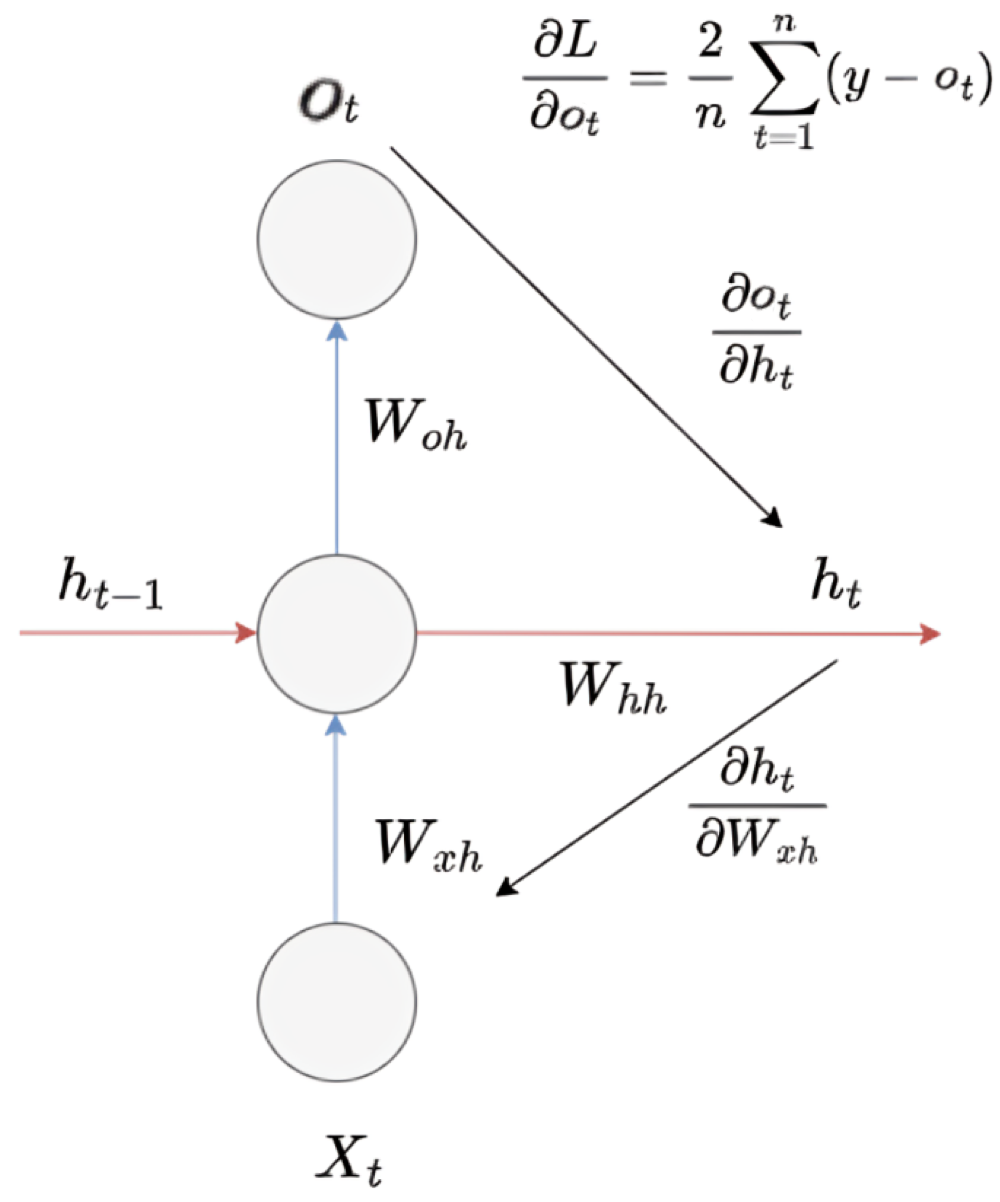
\includegraphics[width=0.4\linewidth]{img/bptt_single3.png}
\caption{Gradient flow in a single time step $t$}
\label{fig:bptt_single}
\end{figure}

Considering the weight matrix $W_{xh}$, in formula, we obtain \cite{medium_math_rnn, quarkml-bptt}:
\begin{equation}
\frac{\partial L}{\partial W_{xh}} = \frac{\partial L}{\partial o_{t}}\frac{\partial o_t}{\partial h_{t}}\frac{\partial h_t}{\partial W_{xh}}
\end{equation}

This formula therefore allows us to calculate the gradient of the loss in relation to the input weights $W_{xh}$ within a \textbf{single time step $t$} \cite{quarkml-bptt}.

When dealing with multiple time steps, it is necessary to sum each individual gradient \cite{quarkml-bptt}.
\begin{figure}[H]
\centering
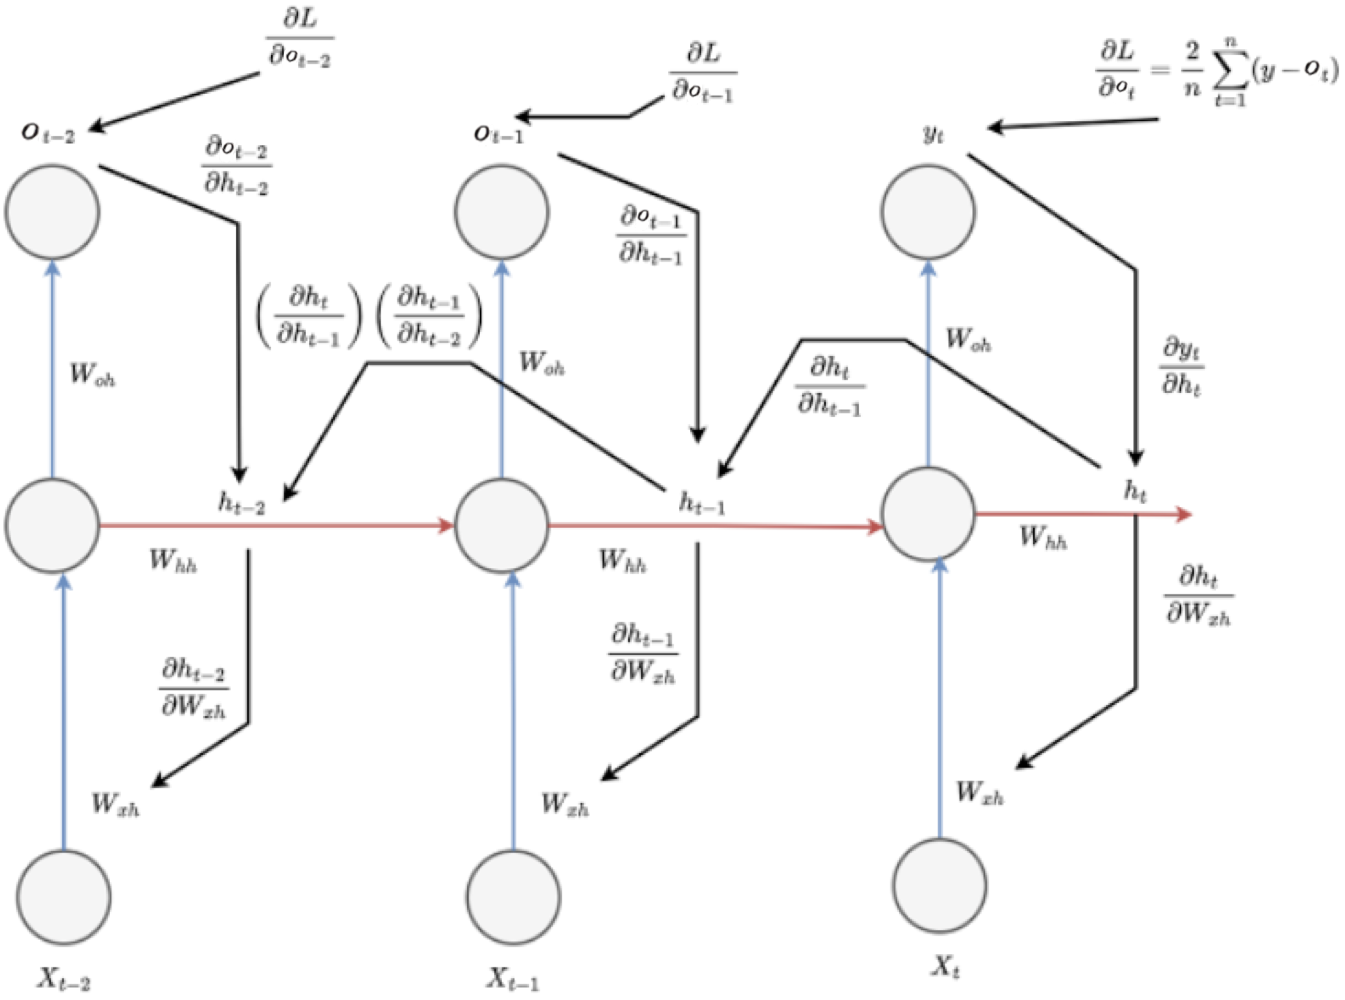
\includegraphics[width=0.8\linewidth]{img/bptt_multiple_2.png}
\caption{Gradient flow over three time steps $t-2, t-1, t$}
\label{fig:bptt_multiple_2}
\end{figure}
Applying the chain rule, we therefore obtain \cite{medium_math_rnn, quarkml-bptt}:
\begin{itemize}
\item \textbf{One time step:}
$$\frac{\partial L}{\partial W_{xh}} = \underbrace{ \frac{\partial L}{\partial o_{t}}\frac{\partial o_t}{\partial h_{t}}\frac{\partial h_t}{\partial W_{xh}}}_{i=0}$$
\item \textbf{Two time steps:} 
$$
\frac{\partial L}{\partial W_{xh}} = 
\underbrace{
\frac{\partial L}{\partial o_t} 
\frac{\partial o_t}{\partial h_t} 
\frac{\partial h_t}{\partial W_{xh}}
}_{i=0} + 
\underbrace{
\frac{\partial L}{\partial o_{t-1}} 
\frac{\partial o_{t-1}}{\partial h_{t-1}} 
\left( \frac{\partial h_t}{\partial h_{t-1}} \right) 
\frac{\partial h_{t-1}}{\partial W_{xh}}
}_{i=1}
$$

\item \textbf{Three time steps:}
$$
\frac{\partial L}{\partial W_{xh}} = 
\underbrace{
\frac{\partial L}{\partial o_t} 
\frac{\partial o_t}{\partial h_t} 
\frac{\partial h_t}{\partial W_{xh}}
}_{i=0} + 
\underbrace{
\frac{\partial L}{\partial o_{t-1}} 
\frac{\partial o_{t-1}}{\partial h_{t-1}} 
\left( \frac{\partial h_t}{\partial h_{t-1}} \right) 
\frac{\partial h_{t-1}}{\partial W_{xh}}
}_{i=1} +
$$
$$
+\underbrace{
\frac{\partial L}{\partial o_{t-2}} 
\frac{\partial o_{t-2}}{\partial h_{t-2}} 
\left( \frac{\partial h_t}{\partial h_{t-1}} \right) 
\left( \frac{\partial h_{t-1}}{\partial h_{t-2}} \right)
\frac{\partial h_{t-2}}{\partial W_{xh}}
}_{i=2}
$$
\end{itemize}

%%%%%%%%%%%%%%%%%%%%%%%%%%%
%Completa questa sezione per bene e poi riparti dai bias
%%%%%%%%%%%%%%%%%%%%%%%%%%%
As the number of time steps increases, the number of gradients increases accordingly. The general formula for calculating $\frac{\partial L}{\partial W_{xh}}$ at time step $t$ is \cite{quarkml-bptt}:
\begin{equation}
\frac{\partial L}{\partial W_{xh}} = \sum_{i=0}^{t} \left[ \underbrace{\frac{\partial L}{\partial o_{t-i}} \frac{\partial o_{t-i}}{\partial h_{t-i}}}_{R_{t-i}} \left( \prod_{j=(t-i+1)}^{t} \frac{\partial h_j}{\partial h_{j-1}} \right) \underbrace{\frac{\partial h_{t-i}}{\partial W_{xh}}}_{S_{t-i}} \right]
\label{eq:grad_wxh}
\end{equation}

where:
\begin{itemize}
\item $o_{t-i}$ represents the output at time step $t-i$
\item $h_{t-i}$ represents the hidden state at time step $t-i$
\item $R_{t-i}$ represents how the variation of the hidden state at time $t-i$ influences the loss through the output at that same instant
\item $S_{t-i}$ represents the direct effect of the weight $W_{xh}$ on the hidden state at time $t-i$
\end{itemize}

To find the derivative of the loss with respect to the weights $W_{hh}$, it is sufficient to replace $W_{xh}$ with $W_{hh}$ in the previous equation, yielding:
\begin{equation}
\frac{\partial L}{\partial W_{hh}} = \sum_{i=0}^{t} \left[ \underbrace{\frac{\partial L}{\partial o_{t-i}} \frac{\partial o_{t-i}}{\partial h_{t-i}}}_{R_{t-i}} \left( \prod_{j=(t-i+1)}^{t} \frac{\partial h_j}{\partial h_{j-1}} \right) \underbrace{\frac{\partial h_{t-i}}{\partial W_{hh}}}_{T_{t-i}} \right]
\end{equation}

where:
\begin{itemize}
\item $T_{t-i}$ represents the extent to which the recurrent weight $W_{hh}$ influences the hidden state at step $t-i$
\end{itemize}

To find the derivative of the output layer weights $W_{oh}$, it is sufficient to consider $o_t$ and $W_{oh}$, resulting in:
\begin{equation}
\frac{\partial L}{\partial W_{oh}} = \sum_{i=0}^{t} \frac{\partial L}{\partial o_{t-i}} \frac{\partial o_{t-i}}{\partial W_{oh}}
\label{eq:grad_woh}
\end{equation}

We now need to find the derivatives of the hidden layer bias $b_h$ and the output layer bias $b_o$.

Regarding the calculation of $b_h$, it is sufficient to replace the matrix $W_{xh}$ with $b_h$ in Equation \ref{eq:grad_wxh}:
\begin{equation}
 \frac{\partial L}{\partial b_{h}} = \sum_{i=0}^{t} \left[ \underbrace{\frac{\partial L}{\partial o_{t-i}} \frac{\partial o_{t-i}}{\partial h_{t-i}}}_{R_{t-i}} \left( \prod_{j=(t-i+1)}^{t} \frac{\partial h_j}{\partial h_{j-1}} \right) \underbrace{\frac{\partial h_{t-i}}{\partial b_{h}}}_{\phi'(a_{t-i})} \right]
\end{equation}

where:
\begin{itemize}
\item $\phi'(a_{t-i})$ represents the derivative of the activation function $\phi$ evaluated at point $a_{t-i}$
\item $a_{t-i}$ is the linear input to the recurrent neuron at time $t-i$, in this case $a_{t-i}=W_{xh}x_{t-i} + W_{hh} h_{t-i-1} + b_h $
\end{itemize}

Similarly, $b_o$ can be found by substituting into Equation \ref{eq:grad_woh}:
\begin{equation}
\frac{\partial L}{\partial b_{o}} = \sum_{i=0}^{t} \frac{\partial L}{\partial o_{t-i}} \frac{\partial o_{t-i}}{\partial b_{o}}
\end{equation}

\paragraph{Weight and Bias Update} The update of weights and biases is performed via gradient descent or one of its optimizers (e.g., Adam) \cite{quarkml-bptt}:
\begin{equation}
 \theta_{k+1} = \theta_k - \eta \nabla L(\theta_k)
\end{equation}

where:
\begin{itemize}
\item $\theta_{k+1}$ represents the vector of updated parameters at iteration $k+1$
\item $\theta_{k}$ represents the vector of parameters at the current iteration $k$
\item $\eta$ represents the learning rate, a positive scalar determining the step size to take in the direction opposite to the gradient
\item $\nabla L(\theta_{k})$ represents the gradient of the cost function $L$ calculated with respect to parameters $\theta_k$. It indicates the direction of steepest ascent of the function.
\end{itemize}

Applying this to the weights $W$ and biases $b$ of the RNN under consideration:

\begin{itemize}
\item \textbf{Updating $\boldsymbol{W_{oh}}$}: 
$$
W_{oh} \leftarrow W_{oh} -\eta \cdot \frac{\partial L}{\partial W_{oh}}
$$

\item \textbf{Updating $\boldsymbol{W_{xh}}$}: 
$$
W_{xh} \leftarrow W_{xh} -\eta \cdot \frac{\partial L}{\partial W_{xh}}
$$

\item \textbf{Updating $\boldsymbol{W_{hh}}$}: 
$$
W_{hh} \leftarrow W_{hh} -\eta \cdot \frac{\partial L}{\partial W_{hh}}
$$

\item \textbf{Updating $\boldsymbol{b_{h}}$}: 
$$
b_{h} \leftarrow b_{h} -\eta \cdot \frac{\partial L}{\partial b_{h}}
$$

\item \textbf{Updating $\boldsymbol{b_{o}}$}: 
$$
b_{o} \leftarrow b_{o} -\eta \cdot \frac{\partial L}{\partial b_{o}}
$$


\end{itemize}

To conclude, the complete pseudocode for BPTT is provided below:

\begin{algorithm}[H]
\caption{Backpropagation Through Time (BPTT)}
\label{alg:bptt}
\small

\begin{algorithmic}[1]

\Inputs
\Statex $\mathbf{a} = (a_0, a_1, \dots, a_{T-1})$ \Comment{Input sequence}
\Statex $\mathbf{y} = (y_0, y_1, \dots, y_{T-1})$ \Comment{Target sequence}
\Statex $N_{epochs}$ \Comment{Maximum number of training epochs}
\Statex $\eta$ \Comment{Learning rate}
\Statex $T$ \Comment{Length of the time sequence}

\Outputs
\Statex $W_{xh}, W_{hh}, W_{oh}, b_h, b_o$ \Comment{Updated weights and biases}

\Initialization
\State Initialize $W_{xh}, W_{hh}, W_{oh}, b_h, b_o$ with small random values.
\State $h_{-1} \leftarrow \mathbf{0}$ \Comment{Initial hidden state (zero)}

\ForAll{$epoch \in \{1, \dots, N_{epochs}\}$}
\Statex \texttt{// ===== FORWARD PASS =====}
\For{$t \in \{0, \dots, T-1\}$}
\State $h_t \leftarrow \tanh(W_{xh} a_t + W_{hh} h_{t-1} + b_h)$ \Comment{Example activation: Tanh}
\State $o_t \leftarrow W_{oh} h_t + b_o$
\State $L_t \leftarrow \frac{1}{2} \| y_t - o_t \|^2$ \Comment{Example loss: Mean Squared Error (MSE)}
\EndFor
\State $L_{total} \leftarrow \sum_{t=0}^{T-1} L_t$ \Comment{Total loss over the sequence}

\Statex
\Statex \texttt{// ===== BACKWARD PASS =====}
\State Initialize gradients: $\nabla W_{xh}, \nabla W_{hh}, \nabla W_{oh}, \nabla b_h, \nabla b_o \leftarrow \mathbf{0}$
\State $\nabla h_{next} \leftarrow \mathbf{0}$ \Comment{Gradient propagated from future step}

\For{$t \in \{T-1, \dots, 0\}$} \Comment{Backpropagation from future to past}
\State $\nabla o_t \leftarrow o_t - y_t$ \Comment{Loss gradient w.r.t. output (for MSE)}

\Statex \texttt{// Compute gradients for output layer}
\State $\nabla W_{oh} \mathrel{+}= \nabla o_t \cdot h_t^T$
\State $\nabla b_o \mathrel{+}= \nabla o_t$

\Statex \texttt{// Backpropagate gradient to hidden layer}
\State $\nabla h_t \leftarrow W_{oh}^T \nabla o_t + \nabla h_{next}$
\State $\nabla h_{raw} \leftarrow (1 - h_t^2) \odot \nabla h_t$ \Comment{Gradient through tanh non-linearity}

\Statex \texttt{// Compute gradients for hidden layer}
\State $\nabla W_{hh} \mathrel{+}= \nabla h_{raw} \cdot h_{t-1}^T$
\State $\nabla W_{xh} \mathrel{+}= \nabla h_{raw} \cdot a_t^T$
\State $\nabla b_h \mathrel{+}= \nabla h_{raw}$

\Statex \texttt{// Update gradient to propagate to previous step}
\State $\nabla h_{next} \leftarrow W_{hh}^T \nabla h_{raw}$
\EndFor

\Statex
\Statex \texttt{// ===== PARAMETER UPDATE =====}
\State $W_{xh} \leftarrow W_{xh} - \eta \cdot \nabla W_{xh}$
\State $W_{hh} \leftarrow W_{hh} - \eta \cdot \nabla W_{hh}$
\State $W_{oh} \leftarrow W_{oh} - \eta \cdot \nabla W_{oh}$
\State $b_h \leftarrow b_h - \eta \cdot \nabla b_h$
\State $b_o \leftarrow b_o - \eta \cdot \nabla b_o$
\EndFor
\end{algorithmic}
\end{algorithm}



\subsection{Limitations and Bottlenecks}
\label{sub:limitazioni}
\noindent
Despite their popularity and adaptability for sequential tasks, Recurrent Neural Networks present certain structural and operational limitations that affect their performance, especially on long sequences or complex data \cite{cs231n-rnn, quarkml-rnn-explained}. The main issues are:

\paragraph{Vanishing Gradient}
The vanishing gradient problem represents the main critical issue in the \textbf{training} of RNNs \cite{analyticsvidhya}. During the BPTT algorithm, weight gradients are multiplied repeatedly for each time step \cite{quarkml-bptt}. In the presence of activation functions such as \textit{sigmoid} or \textit{tanh}, the derivatives, being values between \textbf{\textit{0}} and \textbf{\textit{1}}, tend to progressively reduce the magnitude of the gradients \cite{medium_math_rnn}. This causes the loss of information from further back in the sequence and makes it difficult to learn long-term dependencies \cite{analyticsvidhya}. Consequently, the deeper layers of the network receive negligible updates, limiting the RNN's ability to maintain a ``memory'' of past inputs \cite{cs231n-rnn}.

\paragraph{Exploding Gradient}
Conversely, the exploding gradient problem may occur, where gradients become very large and weights are updated unstably, leading to the divergence of the loss function during training \cite{analyticsvidhya}. This happens less frequently than the vanishing gradient but can still compromise training stability and model quality \cite{medium_math_rnn}. Techniques such as gradient clipping are often used to limit the magnitude of gradients and ensure convergence \cite{quarkml-bptt}.

\paragraph{Limited Long-Term Dependency}
Even without the vanishing gradient, simple RNNs have limited memory and struggle to capture relationships existing between elements of a sequence that are very distant from each other \cite{cs231n-rnn, quarkml-rnn-explained}. This limits performance in applications requiring the understanding of broad contexts, such as the machine translation of long sentences or the analysis of extensive documents \cite{analyticsvidhya}.

\paragraph{Poor Parallelization}
The main limitation regarding the \textbf{parallelization} of RNNs stems from the causal dependency between hidden states, since every $h_t$ requires the computation of $h_{t-1}$, enforcing a strictly sequential processing along the temporal dimension \cite{cs231n-rnn}. During backpropagation through time, this serial nature is also reflected in the \textbf{backward phase}, reducing intra-sequence parallelization, increasing latency per step, and leaving computational resources on GPUs/TPUs underutilized \cite{quarkml-bptt}. Furthermore, training requires maintaining activations over many time steps, resulting in high memory pressure and synchronization costs; truncated BPTT can alleviate the computational load but compromises the learning of long-range dependencies \cite{quarkml-rnn-explained}.

\paragraph{Other Issues}
Other issues mainly include:

\begin{itemize}
\item Optimization Issues \cite{analyticsvidhya}
\item Difficulty in Learning Long and Noisy Sequences \cite{medium_math_rnn}
\end{itemize}

Overall, these criticalities compromise the stability, efficiency, and generalization of RNNs, especially on long and noisy sequences \cite{cs231n-rnn, analyticsvidhya}.



%%%%%%%%%%%%%%%%%%%%%%%%%%%%%%%%%%%%%%%%%%%%%%
% Capitolo 2 %
%%%%%%%%%%%%%%%%%%%%%%%%%%%%%%%%%%%%%%%%%%%%%%

\section{Introduction to the Transformer Architecture}
\label{chap:introduzione}

% \subsection{The Advent of Transformers}
\label{sub:avvento_transformers}
\noindent
The breakthrough came in 2017 with the publication of the paper ``Attention Is All You Need'' by Vaswani et al. \cite{arxiv-attention}, which introduced the Transformer architecture, proposing a completely innovative approach to sequence processing. Unlike previous architectures, Transformers rely entirely on attention mechanisms, thus allowing the model to focus dynamically on the most relevant parts of the input sequence, without the constraints of recurrence or convolution \cite{arxiv-attention, stanford}. This design choice enabled not only greater computational efficiency, thanks to parallelization, but also a remarkable capacity to capture long-range relationships between distant elements in the sequence \cite{arxiv-attention, GeeksForGeeks}.

The impact of the Transformer architecture was immediate and profound: within a few years, it became the new standard for many artificial intelligence applications, ranging from machine translation to the analysis of clinical data and medical images \cite{arxiv-attention, arxiv-skipconnection-survey}. Its flexibility and effectiveness in processing sequential and multimodal data have laid the groundwork for the development of increasingly complex and specialized models, opening new frontiers in the field of AI applied to science and medicine.

\subsection{Theoretical Foundations of the Transformer Architecture}
\label{sec:fondamenti_transformers}
\noindent
The structure of a Transformer can be primarily divided into two macro-areas \cite{arxiv-attention, git-hub}: 
\begin{itemize}
\item \textbf{Encoder:} transforms the input sequence into a contextualized representation \cite{stanford}.
\item \textbf{Decoder:} generates the output sequence using the representation provided by the Encoder \cite{arxiv-attention, stanford}.
\end{itemize}


\begin{figure}[H]
\centering
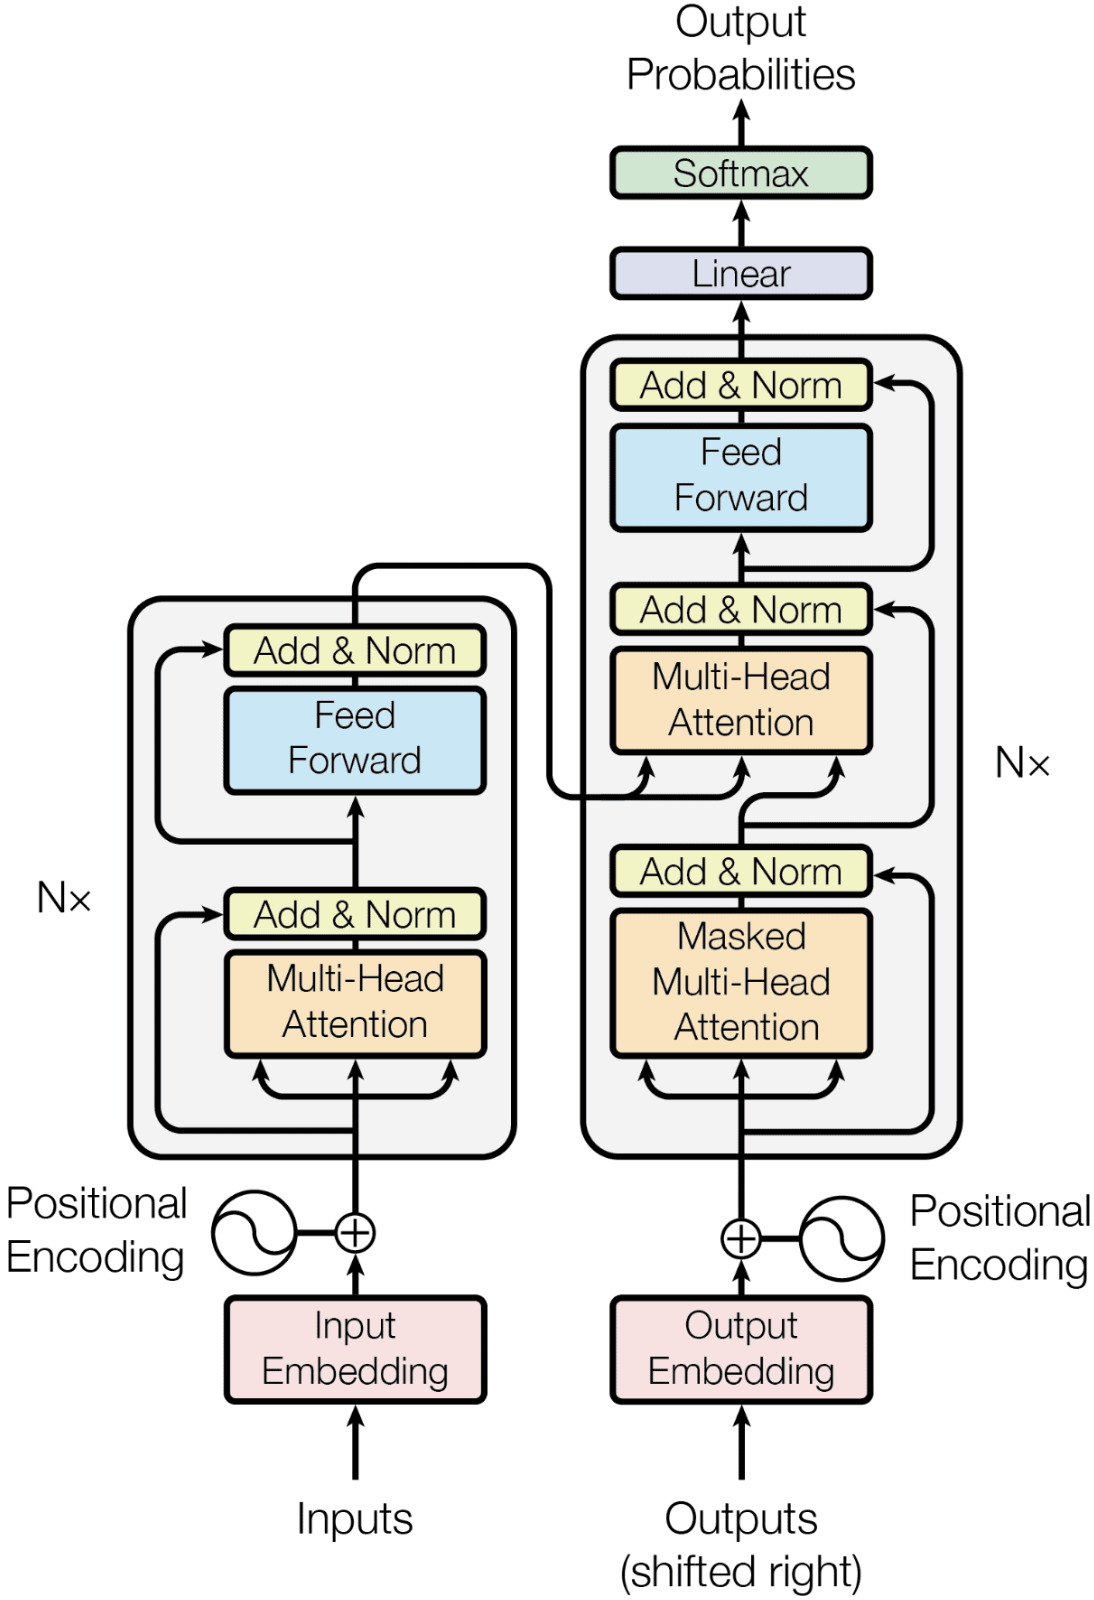
\includegraphics[width=0.5\linewidth]{img/transformer_arch.png}
\caption{Transformer model architecture \cite{arxiv-attention}.}
\label{fig:transformer}
\end{figure}

The figure above shows the original architecture of a Transformer model, as presented in the paper \textit{``Attention Is All You Need''} \cite{arxiv-attention}, comprising all its internal components.
The operation of each of these components is explained below.

%%% Correggere insieme a tutte le volte che dici tokenization
\subsection{Input Representation}
The textual input sequence requires a preprocessing phase to be converted into a compatible numerical format \cite{stanford}. This process consists of three main stages:
\begin{itemize}
\item \textbf{Tokenization} \cite{stanford}
\item \textbf{Input Embedding} \cite{arxiv-attention}
\item \textbf{Positional Encoding} \cite{arxiv-attention, Muhammad_Faizan}
\end{itemize}
These three phases are described below.

\paragraph{Tokenization}
In this first phase, the input sequence—assumed to be textual for simplicity—is divided into multiple sub-sequences called tokens \cite{stanford, git-hub}. Each token belongs to a finite set of strings called the vocabulary $V$ \cite{stanford}. Each token is assigned an integer numerical value corresponding to the position it occupies in the vocabulary \cite{git-hub}.

\begin{figure}[H]
\centering
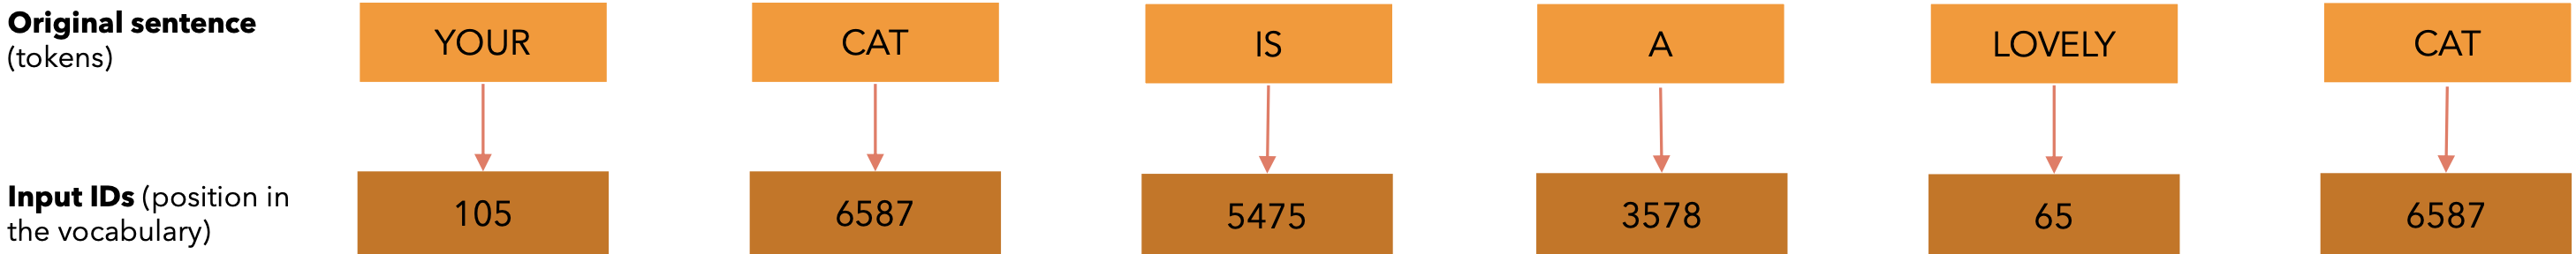
\includegraphics[width=1\linewidth]{img/tokenization.png}
\caption{Representation of the Tokenization phase on the text sequence \textit{"your cat is a lovely cat"} \cite{git-hub}. The input sequence is split into tokens, in this case represented by each word, which are then associated with the corresponding integer in the vocabulary $V$.}
\label{fig:tokenization} % Ho cambiato l'etichetta da placeholder per unicità
\end{figure}

\paragraph{Input Embedding} The numerical values obtained through tokenization are then mapped as vectors of dimension $d_{model}=512$ \cite{arxiv-attention}; every value contained in these vectors is learned during training \cite{git-hub, stanford}. Following these steps, the input text sequence is converted into a series of vectors of $d_{model}$ learned elements called embeddings \cite{arxiv-attention, stanford}.

\begin{figure}[H]
\centering
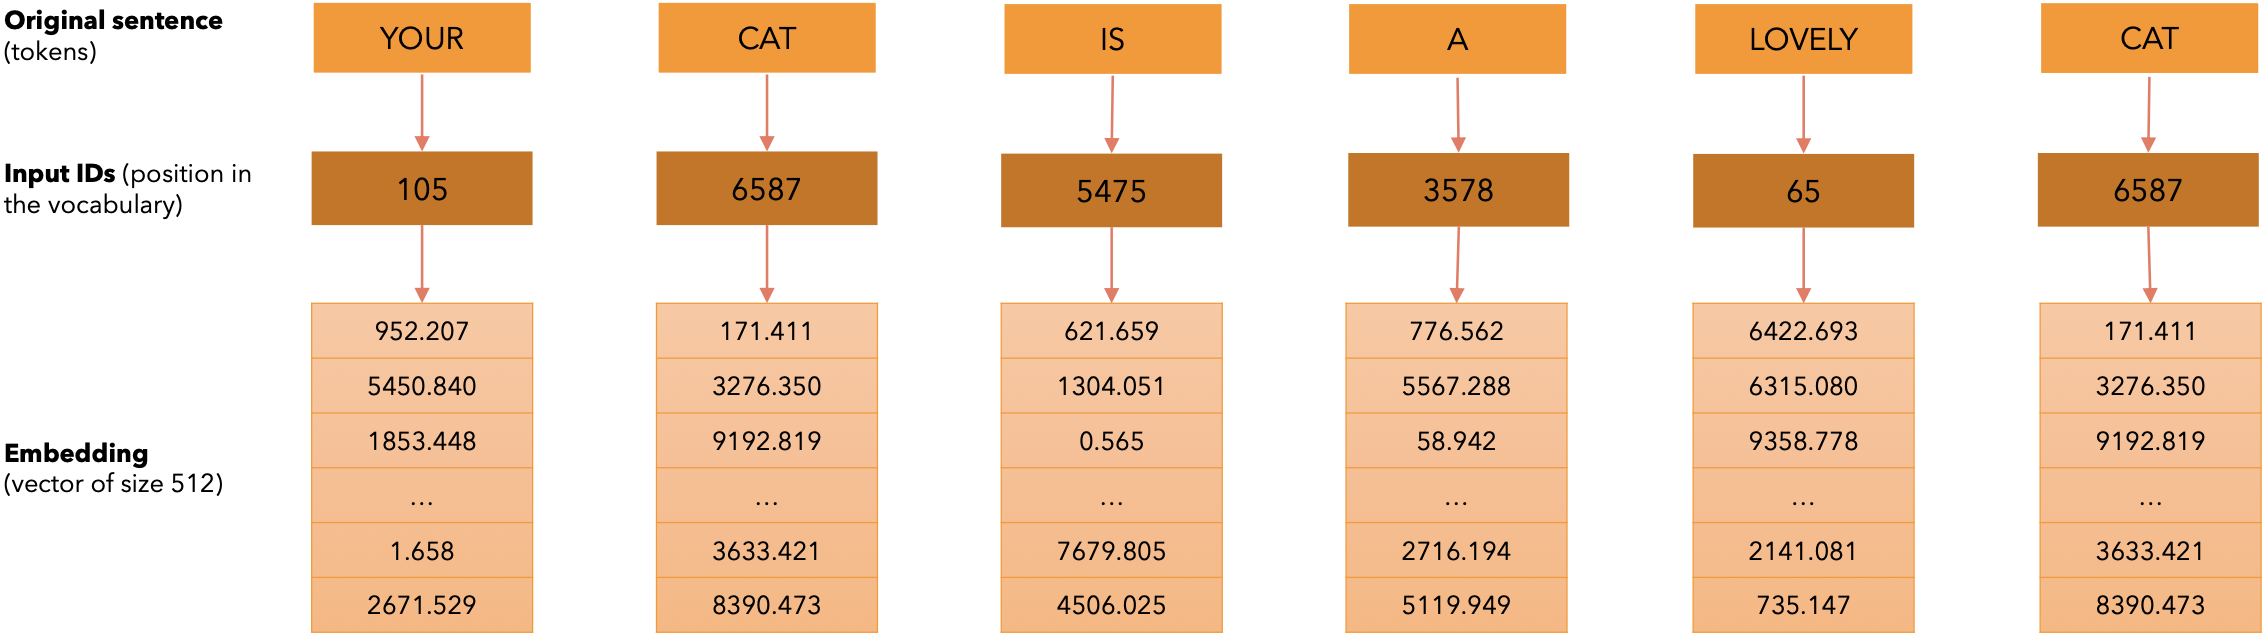
\includegraphics[width=1\linewidth]{img/input_embedding_2.png}
\caption{Representation of the Input Embedding phase \cite{git-hub}.}
\label{fig:embedding}
\end{figure}

\paragraph{Positional Encoding} With the aim of providing order information, each embedding is added to a positional vector $p_{pos} \in \mathbb{R}^{d_{model}}$ \cite{arxiv-attention, Muhammad_Faizan}. 

Each positional vector is calculated as \cite{arxiv-attention}:
\begin{equation}
PE(pos, 2i) = \sin \left(\frac{pos}{10000^{\frac{2i}{d_{model}}}}\right) \quad \textbf{for even \textit{i}}
\end{equation}

\begin{equation}
 PE(pos, 2i+1) = \cos \left(\frac{pos}{10000^{\frac{2i}{d_{model}}}}\right) \quad \textbf{for odd \textit{i}}
\end{equation}

where \cite{Muhammad_Faizan, git-hub}:
\begin{itemize}
\item $pos$ represents the index of the position vector within the sequence
\item $i$ represents the position of the element within the vector $pos$
\end{itemize}

\begin{figure}[H]
\centering
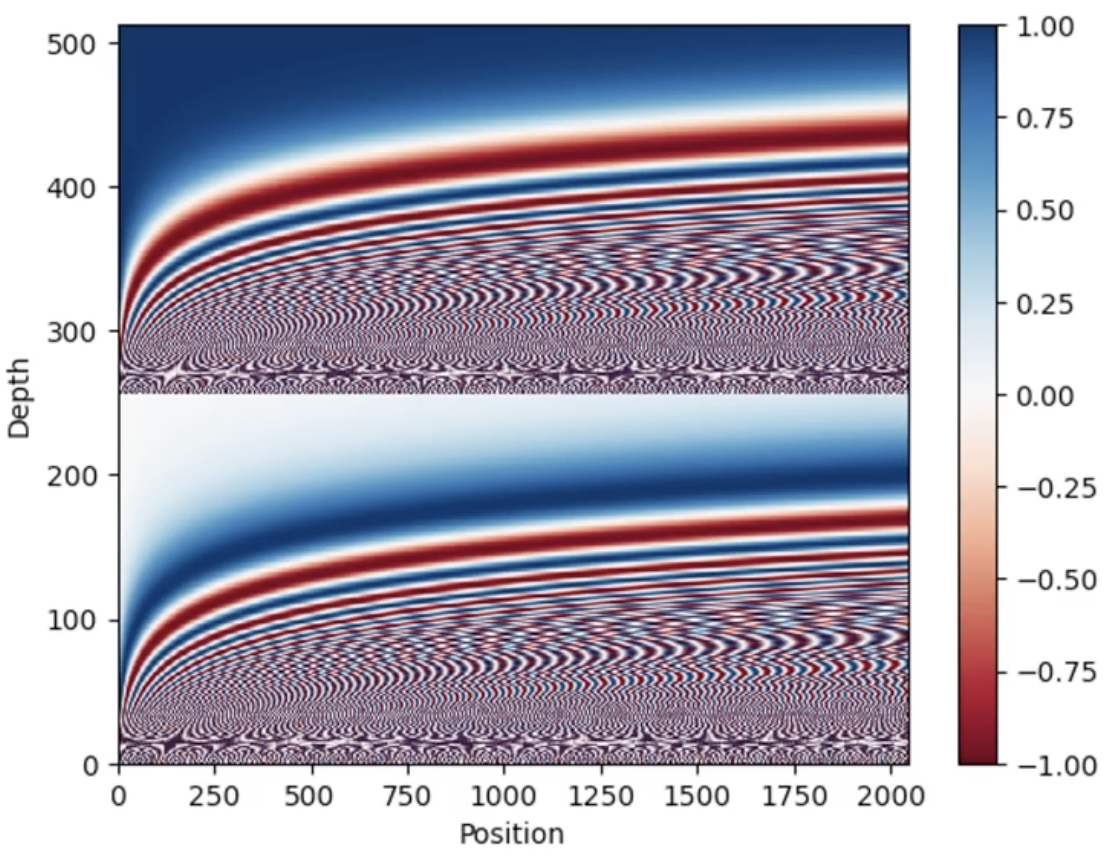
\includegraphics[width=0.5\linewidth]{img/positional_encoding_graphic.png}
\caption{Visualization of the sinusoidal positional encoding matrix for a model with $d_{model}=512$ \cite{git-hub}. The horizontal axis represents the token position in the sequence, while the vertical axis indicates the encoding vector dimension \cite{git-hub}. The color encodes the value of the sine function, which ranges from -1 to +1 \cite{Muhammad_Faizan, git-hub}.}
\label{fig:pos_encoding}
\end{figure}

The sine and cosine functions were chosen for positional encoding calculation because they offer a combination of properties ideal for representing order in a non-recurrent architecture \cite{arxiv-attention, Muhammad_Faizan}:
\begin{itemize}
\item \textbf{Positional Uniqueness:} Each position in the sequence has a unique positional encoding vector \cite{Muhammad_Faizan}. The combination of sine waves at different frequencies (controlled by the term $10000^\frac{2i}{d_{model}}$) ensures that no two positions share the exact same encoding vector \cite{arxiv-attention}.
\item \textbf{Relative Position Representation:} For a fixed distance $k$, the encoding vector at position $pos + k$ can be represented as a linear transformation of the vector at position $pos$ \cite{arxiv-attention}. This allows the model to easily learn to recognize relative positions, independently of the absolute position \cite{Muhammad_Faizan}. The attention mechanism, being based on dot products (a linear transformation), can directly leverage this property \cite{git-hub}.
\item \textbf{Generalization to Longer Sequences:} Since sine and cosine functions are periodic and their behavior is well-defined outside the training interval, the model can extrapolate to sequences longer than those seen during training \cite{arxiv-attention, Muhammad_Faizan}.
\item \textbf{Bounded Values and Stability:} Sine and cosine values are naturally bounded within the interval $\left[-1,1\right]$, which helps keep embedding values normalized and contributes to numerical stability during training \cite{Muhammad_Faizan}.
\end{itemize}
The positional embeddings are then added to the corresponding embeddings \cite{arxiv-attention}.
The result of this operation constitutes the input to the Encoder \cite{git-hub, stanford}.

\begin{figure}[H]
\centering
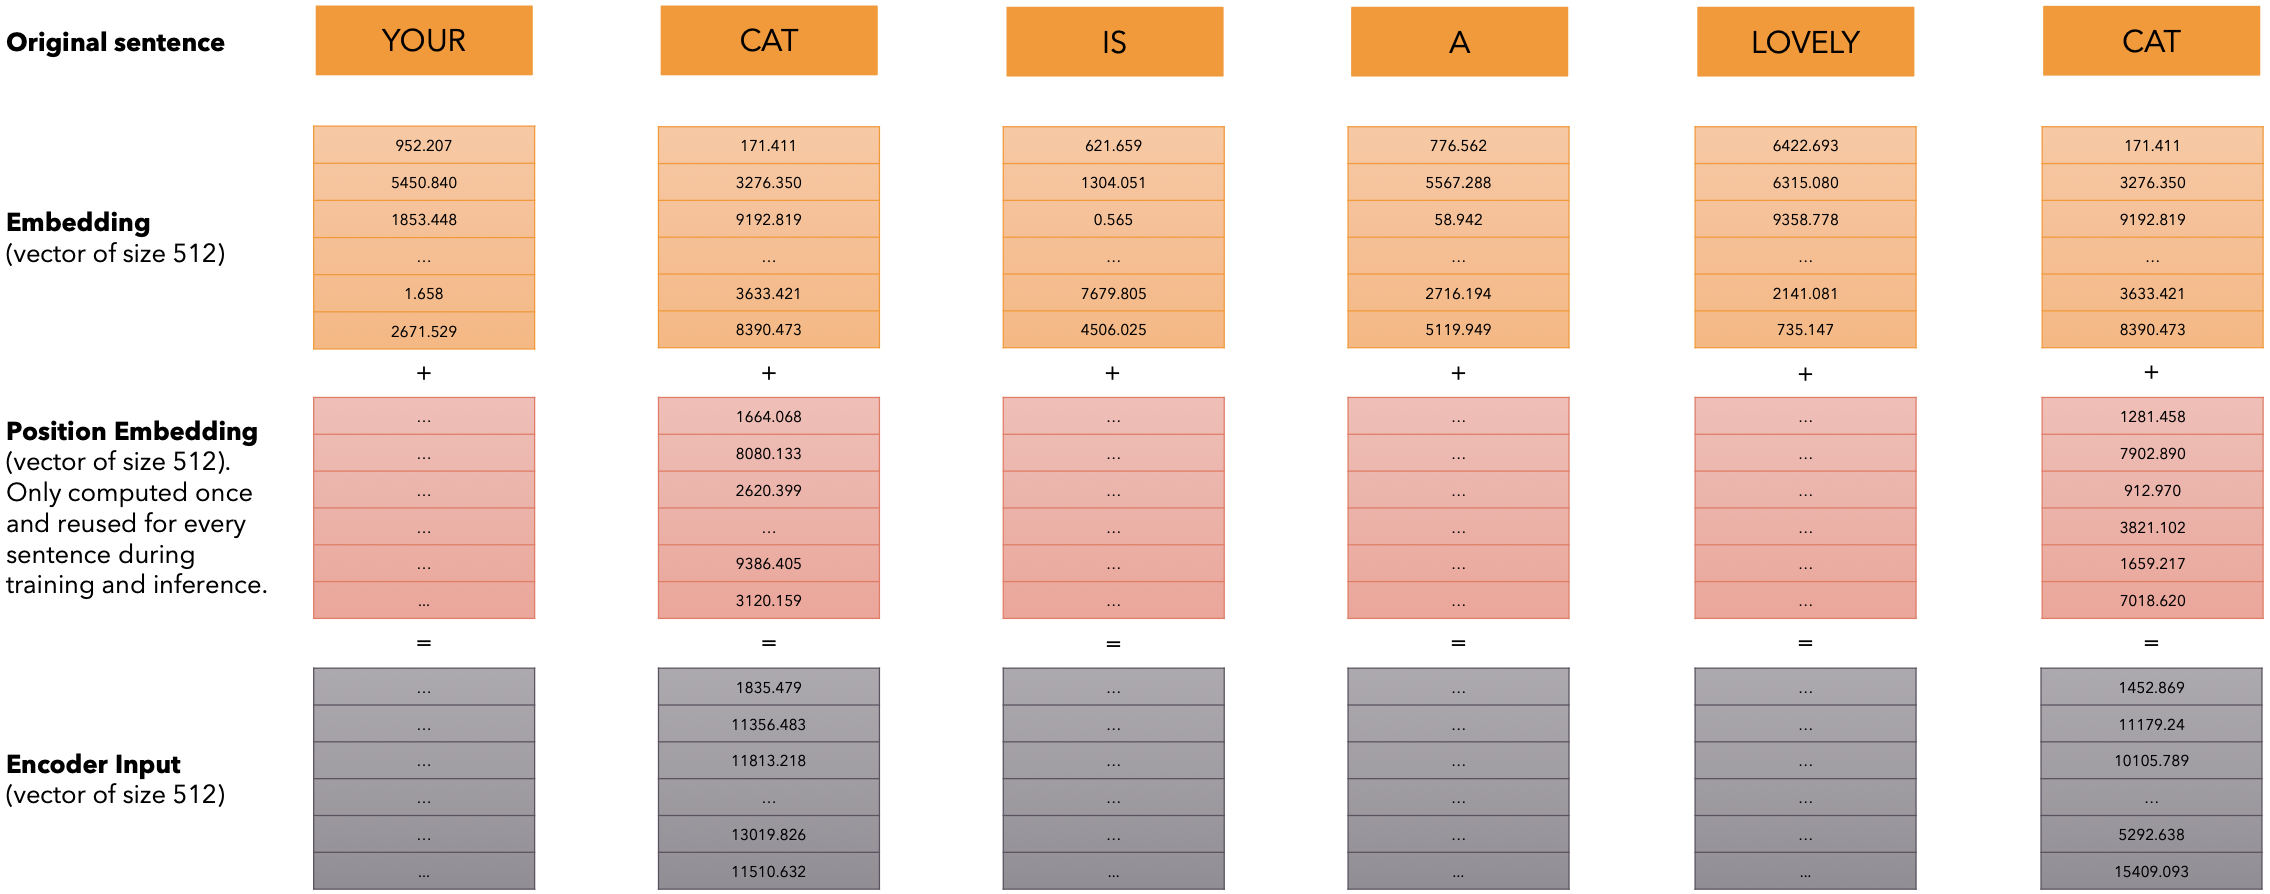
\includegraphics[width=1\linewidth]{img/tokenization_summary.png}
\caption{Summary scheme of Input Representation via Tokenization, Input Embedding, and Positional Encoding \cite{git-hub}.}
\label{fig:input_summary}
\end{figure}

\subsection{Self-Attention}
The fundamental component of the Transformer architecture is the self-attention mechanism \cite{arxiv-attention, stanford}. Unlike recurrent models that process sequences serially, self-attention allows the model to weigh the importance of each token within a sequence in relation to all others, capturing contextual dependencies independently of their distance \cite{arxiv-attention, GeeksForGeeks}. 

The computation of self-attention, considered here as single-head, is based on a function called Scaled Dot-Product Attention \cite{arxiv-attention}. Formally, the input to this mechanism consists of three matrices \cite{arxiv-attention, hashnode}:
\begin{itemize}
\item \textbf{Query Matrix} $\rightarrow \quad Q \in \mathbb{R}^{seq \times d_{k} }$ 
\item \textbf{Key Matrix} $\rightarrow \quad K \in \mathbb{R}^{seq \times d_{k} }$
\item \textbf{Value Matrix} $\rightarrow \quad V \in \mathbb{R}^{seq \times d_{v} }$
\end{itemize}
Where \cite{arxiv-attention, git-hub}:
\begin{itemize}
\item $seq$ represents the length of the input sequence
\item $d_k, d_v$ are the dimensions of the representations
\end{itemize}
These three matrices are obtained by projecting the input matrix $ X \in \mathbb{R}^{seq \times d_{model}}$, constructed by stacking the input representation vectors, via three distinct weight matrices $W^Q \in \mathbb{R}^{d_{model} \times d_{k}}, W^K\in \mathbb{R}^{d_{model} \times d_{k}}$, and $W^V\in \mathbb{R}^{d_{model} \times d_{v}}$ learned during training \cite{arxiv-attention, hashnode, stanford}:
\begin{equation}
Q=XW^Q, \quad K= XW^K,\quad V=XW^V 
\end{equation}

The Scaled Dot-Product Attention function is then calculated as follows \cite{arxiv-attention}:
\begin{equation}
Attention(Q, K, V)=softmax\left(\frac{QK^T}{\sqrt{d_k}}\right)V
\end{equation}

This operation produces the so-called attention matrix \cite{arxiv-attention, hashnode}. \footnote{The scaling factor $\frac{1}{\sqrt{d_k}}$ is crucial \cite{arxiv-attention}. Without it, for large values of $d_k$, the dot products can grow large in magnitude, pushing the softmax function into regions where it has extremely small gradients (vanishing gradients) \cite{git-hub, arxiv-attention}. This would effectively halt the training process \cite{arxiv-attention}.}
\begin{figure}[H]
\centering
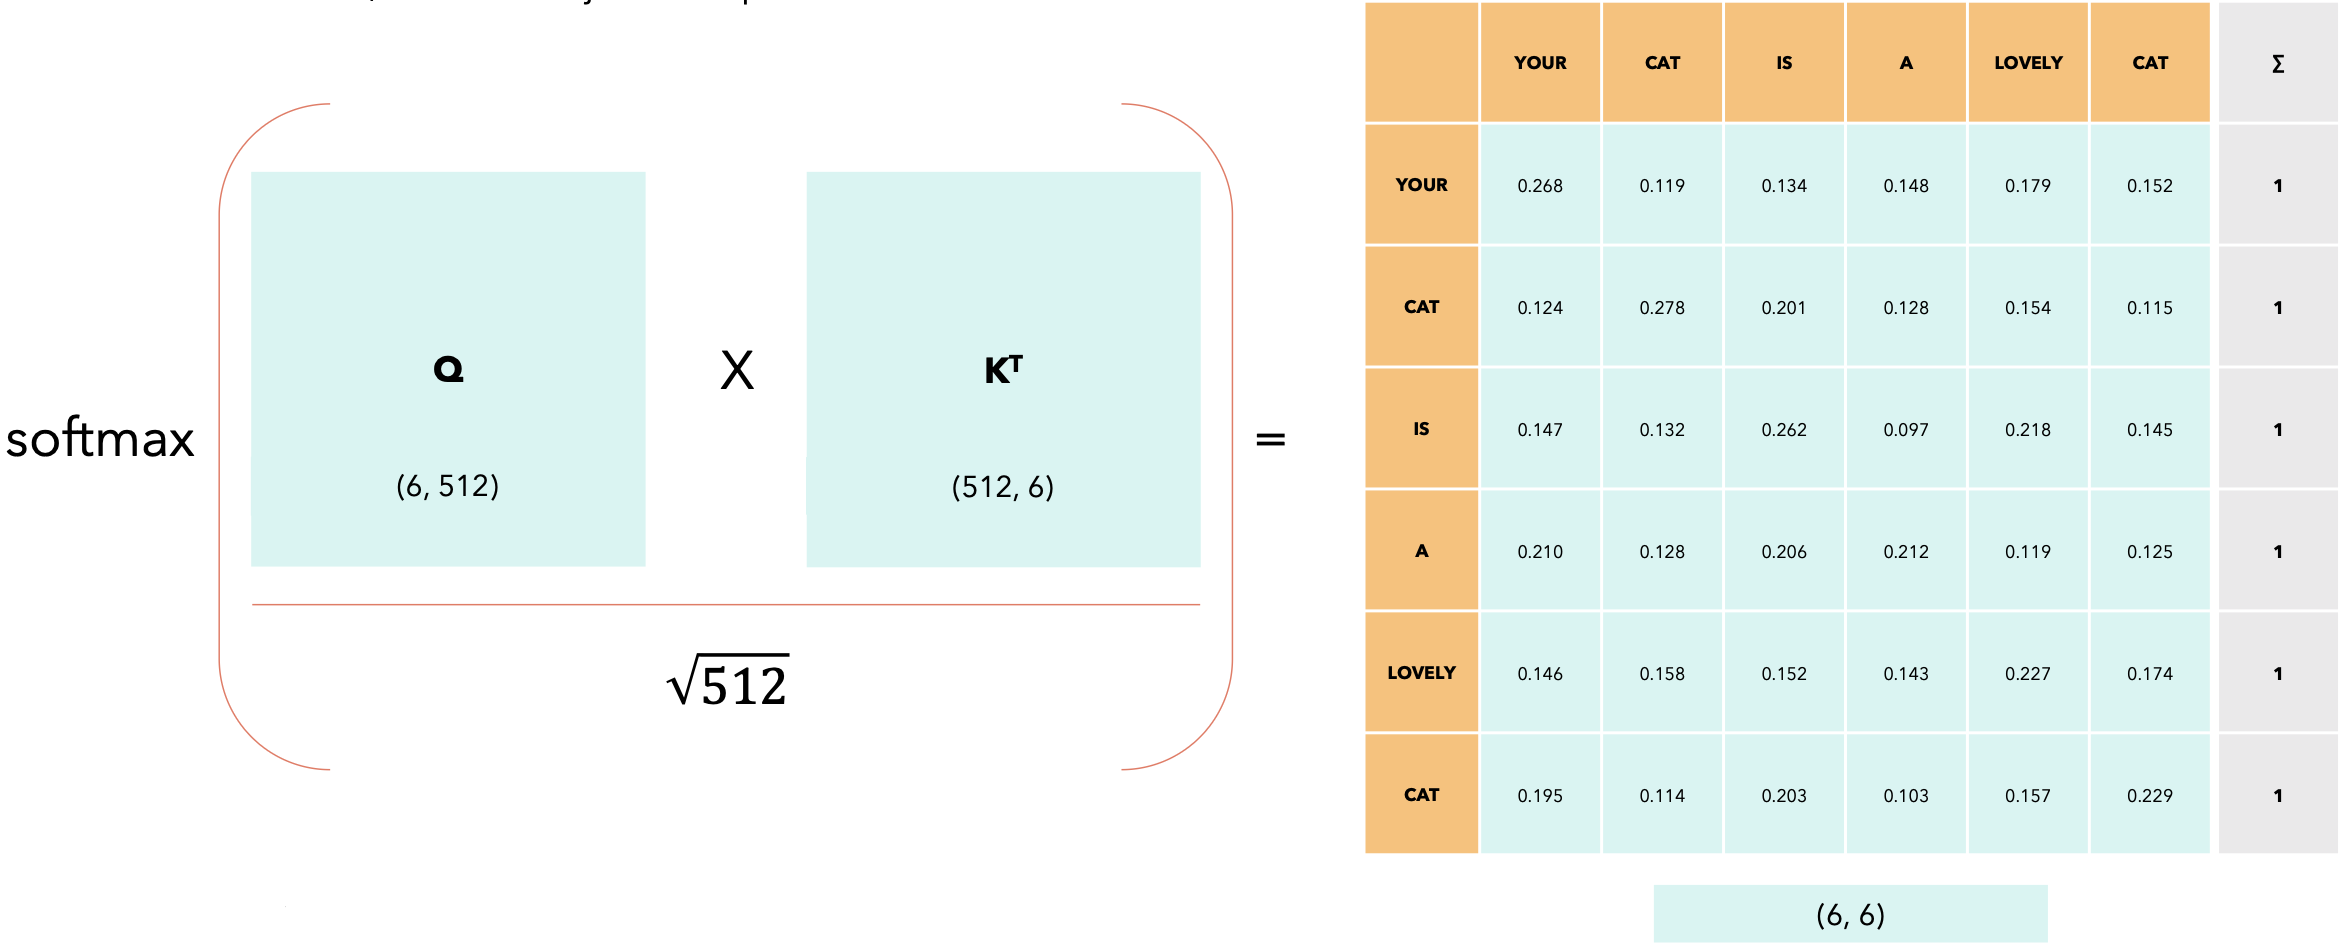
\includegraphics[width=1\linewidth]{img/self_attention.png}
\caption{Softmax of the Scaled Dot-Product Attention calculated by setting, for simplicity, $d_k=d_v=d_{model}=512$, $seq=6$, and following the previous examples \cite{git-hub}. Note how, thanks to the \textit{softmax}, the sum of each row is 1.}
\label{fig:self_attention_softmax}
\end{figure}

\begin{figure}[H]
\centering
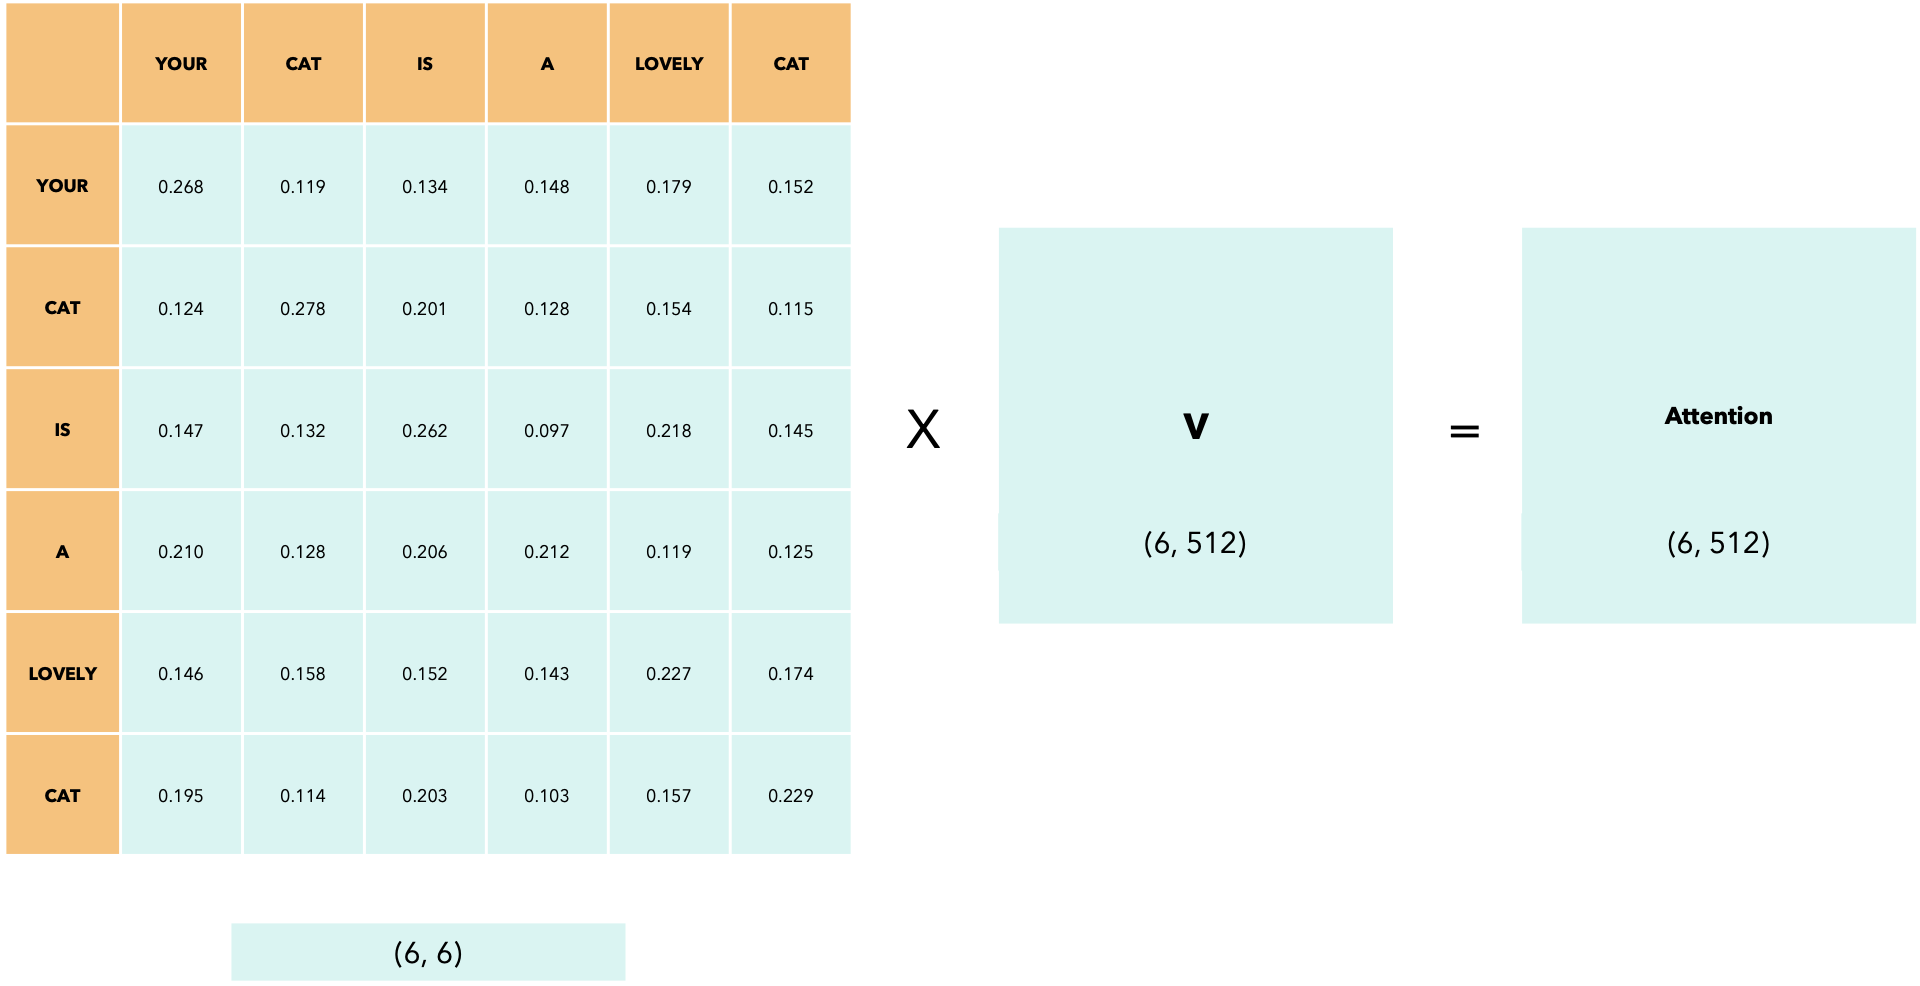
\includegraphics[width=1\linewidth]{img/self_attention_result.png}
\caption{Result of the Scaled Dot-Product Attention introduced in the previous figure. Each row of the resulting attention matrix will capture not only the meaning (thanks to the embedding) and the position in the sequence (thanks to the positional encoding) but also every interaction of each token with the other tokens \cite{git-hub}.}
\label{fig:self_attention_result}
\end{figure}

\subsubsection{In-depth Analysis of Q, K, and V Matrices}
The Query, Key, and Value matrices play distinct and complementary roles in the attention calculation process, allowing the model to effectively weigh the importance of each token in the sequence relative to the others \cite{arxiv-attention, stanford, git-hub}.
To better understand the role of the individual matrices, an analogy can be used \cite{hashnode, GeeksForGeeks}: \textit{Imagine being in a library and wanting to find books on a particular topic.}
We can structure the situation as follows:
\begin{itemize}
\item \textbf{Query (Q):} Represents the question we ask. For example: \textit{"I am looking for books on Renaissance art history."} The query encodes what we are looking for, the important features in our case.
\item \textbf{Key (K):} Represents the labels or cataloging of the books. Each book has metadata stating: \textit{"This book is about: history, art, Renaissance, France, 1500."} The keys make the books "searchable."
\item \textbf{Value (V):} Represents the actual content of the books. Once we find the books that match our searches, i.e., with \textbf{high similarity between Q and K}, we retrieve their content to read and understand.
\end{itemize}

We can therefore describe, more formally, the semantic role of each of these three matrices.

\paragraph{Semantic Role of the Query} The Query represents, as mentioned, the "question" that each token poses to the rest of the sequence \cite{arxiv-attention, stanford}. Concretely, the query vector $q_i=x_iW^Q$ of a token $i$ encodes what information that token is seeking from other words in the sequence to better understand its own meaning within the context \cite{hashnode, GeeksForGeeks}. For example, in a sentence like \textit{"The cat meows"}, the token \textit{"cat"} might have a query that "looks for" information about actions it performs (represented by the key of \textit{"meows"}) or determinants that qualify it (represented by the key of \textit{"The"}).
Formally, during the attention calculation, the query of token $i$ is compared with the keys of all tokens via the dot product, thus measuring the compatibility between what token $i$ is looking for and what the other tokens offer \cite{arxiv-attention, git-hub}.

\paragraph{Semantic Role of the Key} The Key represents the "search labels" or "identifying metadata" of each token \cite{hashnode, GeeksForGeeks}. The key vector $k_j=x_jW^K$ of a token $j$ encodes which characteristics make that token identifiable and searchable by tokens seeking information \cite{arxiv-attention}. The key of a token exposes the salient traits that distinguish it and make it relevant in different contexts. The role of the key is crucial in determining relevance: every query of every token is compared (via dot product) with the key of every other token \cite{arxiv-attention, stanford}. A high value of $q_i \cdot k_j$ indicates that token $j$ contains information that token $i$ is looking for, and therefore deserves a high attention weight \cite{git-hub}.

\paragraph{Semantic Role of the Value} The Value represents the actual semantic content that each token contributes to the contextualized representation of the other tokens \cite{arxiv-attention, stanford}. The value vector $v_j=x_jW^V$ of a token $j$ encodes the intrinsic meaning of the token, suitably transformed to be combinable with the values of other tokens \cite{hashnode, GeeksForGeeks}.

Unlike Query and Key, which are used to calculate attention weights, the Value is combined according to these weights \cite{arxiv-attention}. By decomposing the Scaled Dot-Product Attention into two phases:
\begin{equation*}
    AttentionWeights=softmax\left( \frac{QK^T}{\sqrt{d_k}} \right) \quad \tag{Phase 1}
\end{equation*}
where $AttentionWeights$ results in a matrix in $\mathbb{R}^{seq\times seq}$ containing the attention weights \cite{arxiv-attention, git-hub}. The element $(i,j)$ of this matrix therefore indicates how much token $i$ should attend to element $j$ of the sequence.

\begin{equation*}
Attention=AttentionWeights\cdot V \tag{Phase 2}
\end{equation*}
where $Attention \in \mathbb{R}^{seq \times d_V}$ contains the final output of the attention mechanism, in which each row $z_i$ represents token $i$ contextualized within the input sequence \cite{arxiv-attention}.

The contextualized representation of each single token is therefore obtained as a weighted sum of all the value vectors of the sequence \cite{stanford, git-hub}:
\begin{equation}
z_i=\sum^n_{j=1}AttentionWeights_{ij}\cdot v_j
\end{equation}

\subsubsection{Properties of the Self-Attention Mechanism}
The characteristics of Self-Attention include:
\begin{itemize}
\item \textbf{Permutation Equivariance:} A function $f:\mathbb{R}^{n\times d} \rightarrow \mathbb{R}^{n\times d}$ is permutation equivariant if, for any input matrix $X \in \mathbb{R}^{n\times d}$ and any permutation matrix $P_\pi \in \mathbb{R}^{d\times d}$ (which permutes the rows of $X$), the following holds \cite{arxiv-permutation-equivariance-transformers}:
\begin{equation}
f(P_\pi X) = P_\pi f(X)
\end{equation}
This implies that if the rows of the input matrix $X$ are permuted, the rows of the output attention matrix will be permuted in the same manner \cite{arxiv-permutation-equivariance-transformers, git-hub}.

Although this property ensures that the model does not arbitrarily favor specific positions in the sequence, it presents a critical aspect: without further mechanisms, the model would be insensitive to the sequence order \cite{arxiv-permutation-equivariance-transformers}. Two identical sequences in different orders—for example, \textit{"Riccardo greets Alice"} and \textit{"Alice greets Riccardo"}—would produce numerically equivalent (albeit permuted) outputs \cite{arxiv-permutation-equivariance-transformers}. To address this issue, the Transformer introduces positional encoding, which adds explicit positional information to each token \cite{arxiv-permutation-equivariance-transformers, git-hub, arxiv-attention}, effectively breaking permutation equivariance and allowing the model to capture and represent dependencies related to the sequence order \cite{arxiv-permutation-equivariance-transformers}.

\item \textbf{Long-Range Dependency Modeling:} Unlike recurrent networks, where information must traverse all intermediate steps sequentially, self-attention reduces the maximum signal path length to a constant value of $O(1)$ \cite{arxiv-attention, stanford}. This allows for directly connecting every pair of tokens regardless of their positional distance, facilitating the learning of global semantic relationships \cite{arxiv-attention, GeeksForGeeks}.

\item \textbf{Full Parallelizability:} In contrast to Recurrent Neural Networks (RNNs), self-attention consists exclusively of matrix multiplications, allowing for total parallelization on \textit{GPUs} \cite{arxiv-attention, git-hub}.

\item \textbf{Computational Complexity:} It has a time complexity of $O(seq^2d_{model})$ and a memory complexity of $O(seq^2)$ \cite{arxiv-attention, arxiv-attention, stanford}, \footnote{This quadratic complexity represents a significant bottleneck in the medical domain, where inputs such as Electronic Health Records (EHRs) or genomic sequences can be extremely long \cite{pmc-timelygpt}. This limitation has led to the development of "efficient Transformers" (e.g., Longformer, BigBird) specifically designed to handle long contexts with linear or log-linear complexity \cite{arxiv-efficient-transformers}.} making it efficient for sequences of moderate length but prohibitive for very long sequences \cite{arxiv-attention}.

\item \textbf{Differentiability:} All components are differentiable, allowing training via backpropagation without non-derivable components \cite{arxiv-attention, git-hub}.
\end{itemize}

\subsection{Multi-head Attention}
The self-attention mechanism, described in the previous section, computes a single contextualized representation for each token via a single attention operation. However, this architecture limits the model's ability to simultaneously capture different types of relationships between tokens \cite{arxiv-attention, stanford, git-hub}. For instance, the model might need to identify grammatical agreements (where a verb should attend to the subject), positional proximity relationships, or semantic similarities, all concurrently \cite{GeeksForGeeks}. A single linear transformation cannot effectively represent all these dimensions of meaning simultaneously \cite{git-hub}. The solution proposed in the paper \textit{"Attention Is All You Need"} is the Multi-Head Attention mechanism, which allows the model to perform attention calculations in parallel \cite{arxiv-attention}. Each attention "head" learns to specialize in extracting a different type of contextual relationship, and the outputs of all heads are subsequently combined \cite{arxiv-attention, stanford}.
\begin{figure}[H]
\centering
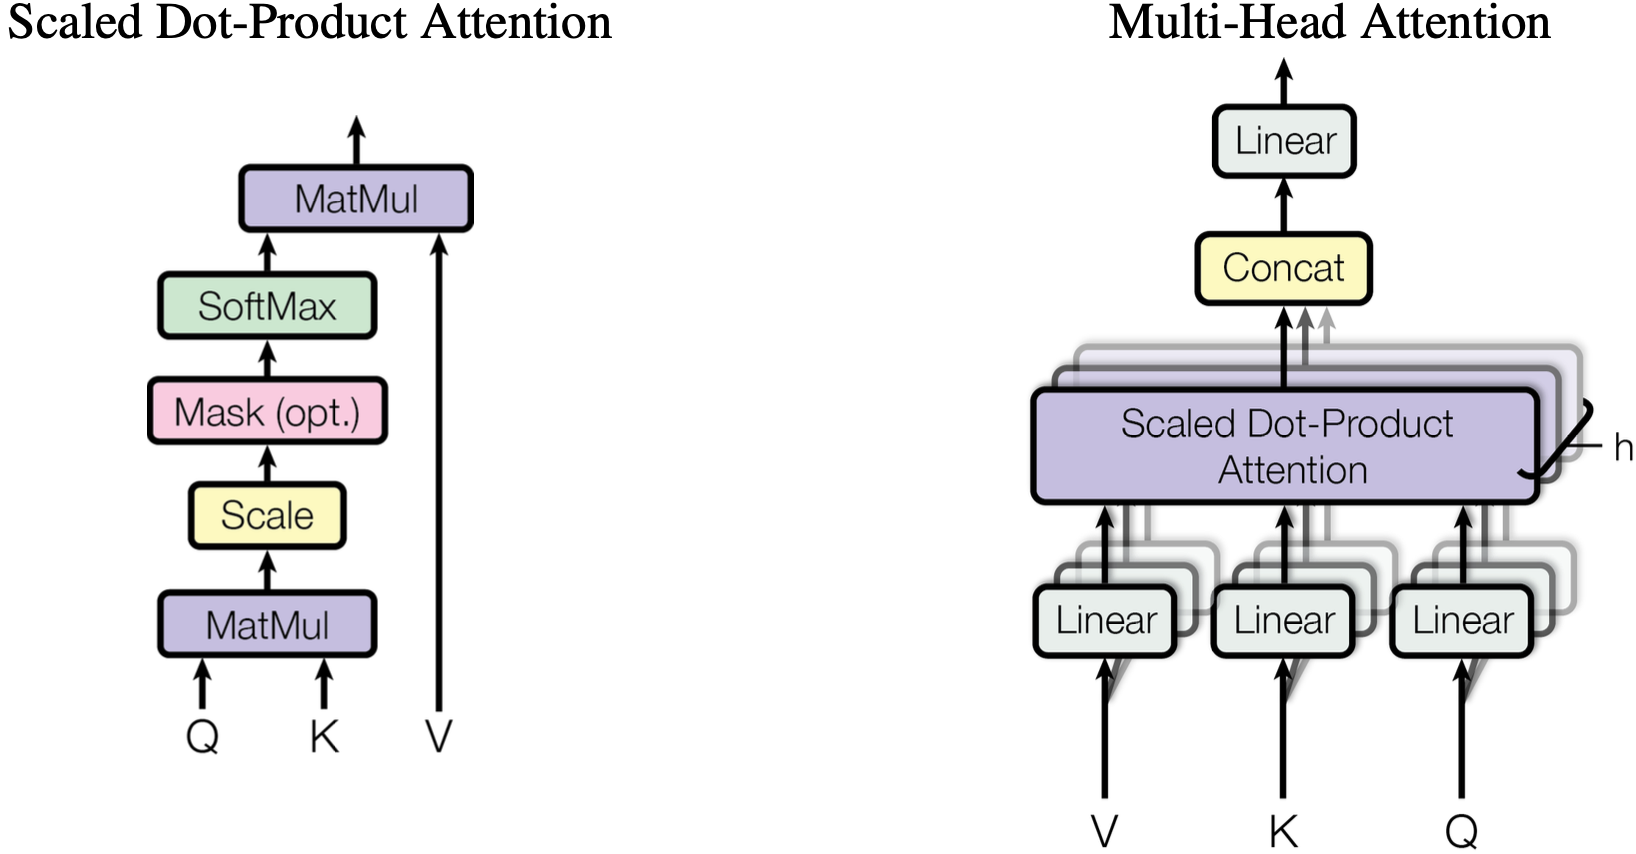
\includegraphics[width=1\linewidth]{img/multi-and-single-head.png}
\caption{On the left is a schematic representation of Scaled Dot-Product Attention (single-head) \cite{arxiv-attention}. On the right is a schematic representation of Multi-Head Attention consisting of several Attention layers in parallel \cite{arxiv-attention}.}
\label{fig:scaled_dot}
\end{figure}

\subsubsection{Hyperparameter Specification}
Let $h$ be the number of attention heads (a hyperparameter, typically 8 or 16 in standard models) \cite{arxiv-attention, stanford}. In the original paper, to ensure the computational cost remains manageable, the dimensions are set as \cite{arxiv-attention}:
\begin{equation}
d_k=d_v=\frac{d_{model}}{h}
\end{equation}

For each head $i\in\{1, 2, \dots, h\}$, three independent weight matrices are defined, which are learned during training \cite{arxiv-attention, git-hub}:
$$
W^Q_i\in \mathbb{R}^{d_{model}\times d_k}, W^K_i\in \mathbb{R}^{d_{model}\times d_k}, W^V_i\in \mathbb{R}^{d_{model}\times d_v}
$$
Additionally, a final output weight matrix \cite{arxiv-attention}:
$$
W^O \in \mathbb{R}^{(h\cdot d_v)\times d_{model}}
$$

\subsubsection{Operational Flow}
\paragraph{Linear Projections per Head}
The input matrix $X \in \mathbb{R}^{seq\times d_{model}}$, produced by tokenization, is projected into Query, Key, and Value for each head $i=\{1,\dots,h\}$ \cite{arxiv-attention, stanford}:
\begin{equation}
Q_i=XW^Q_i, K_i=XW^K_i, V_i=XW^V_i
\end{equation}

where:
\begin{itemize}
\item $Q_i=XW^Q_i \in \mathbb{R}^{seq\times d_{k}},$ represents the Query matrix corresponding to head $i$
\item $K_i=XW^K_i \in \mathbb{R}^{seq\times d_{k}},$ represents the Key matrix corresponding to head $i$
\item $V_i=XW^V_i \in \mathbb{R}^{seq\times d_{v}},$ represents the Value matrix corresponding to head $i$
\end{itemize}
This operation will therefore yield a set of $h$ distinct Query, Key, and Value matrices \cite{arxiv-attention, git-hub}. \footnote{From an implementation perspective (e.g., in frameworks like PyTorch \cite{pytorch-multiheadattention} or TensorFlow \cite{tensorflow-multiheadattention}), these projections are rarely performed as a loop over $h$ separate matrices \cite{stanford}. Instead, a single large weight matrix (of size $d_{model} \times d_{model}$) is used to project the input at once, and the resulting tensor is subsequently reshaped to separate the heads \cite{stanford, git-hub}. This "vectorized" approach leverages GPU parallelism to maximize efficiency, while producing a mathematically equivalent result to the separate formulation \cite{stanford}. The figures in this section illustrate this efficient implementation strategy (labeled as \textit{"Alternative Approach"}) \cite{git-hub, stanford}.}

Since each head possesses distinct weight matrices, the input is "viewed" from multiple different perspectives, allowing for the extraction of different semantic structures from the input \cite{arxiv-attention, stanford, git-hub}.
\begin{figure}[H]
\centering
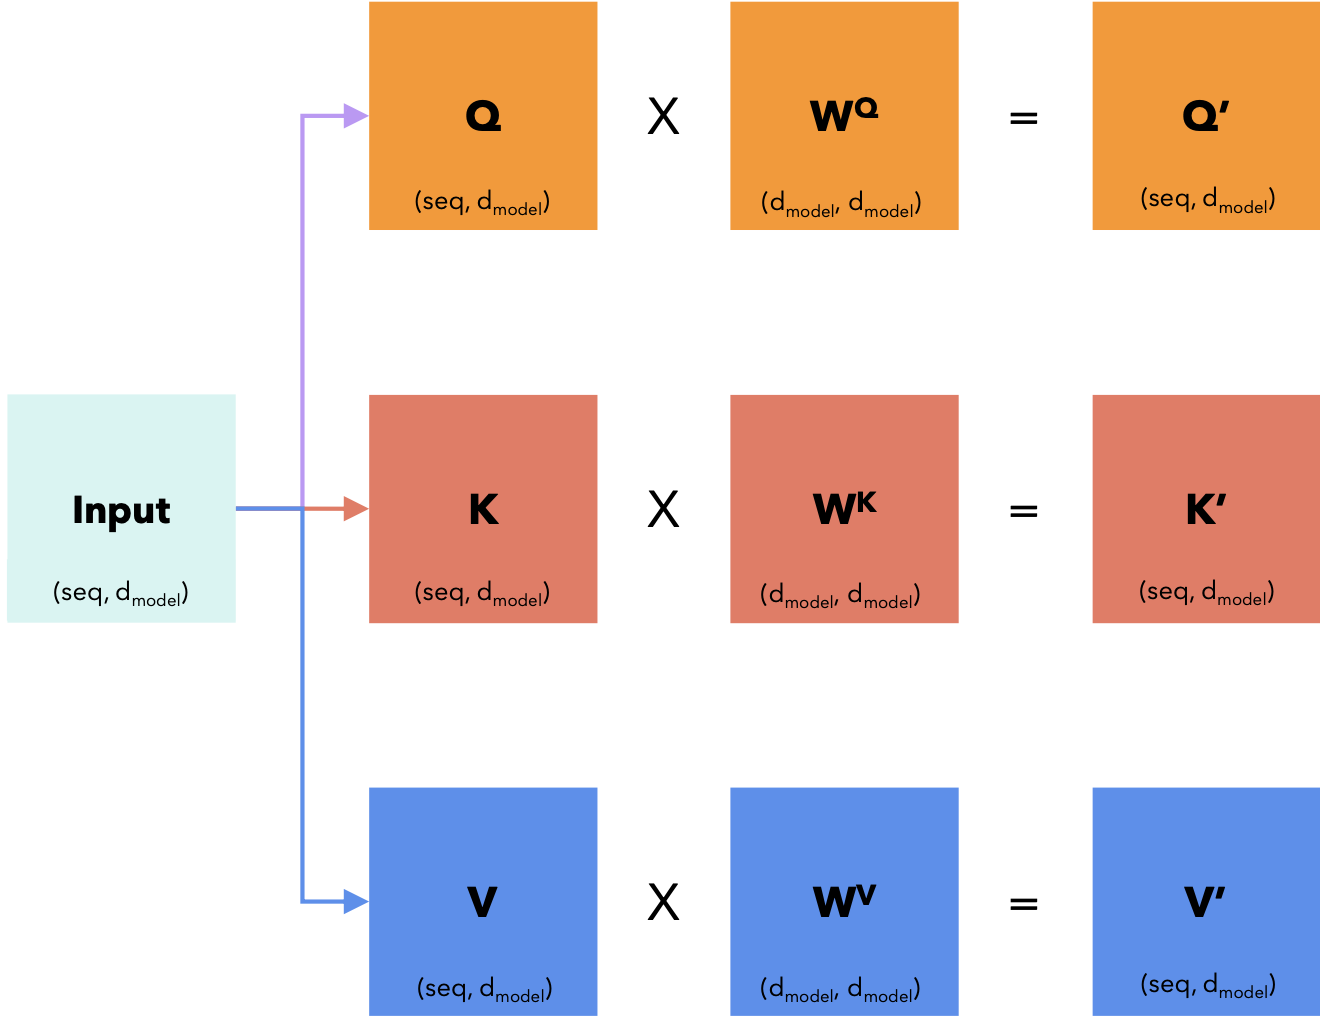
\includegraphics[width=0.8\linewidth]{img/Proiezioni_Lineari_mh.png}
\caption{\textbf{(Alternative Approach, \textit{Step 1})} Graphical representation of the linear projection calculation for $Q, K$, and $V$ \cite{git-hub}. In this case, for efficiency reasons, three matrices $W$ of dimension $d_{model}\times d_{model}$ (thus larger) are considered and projected a single time onto $K, V$, and $Q$. The matrices resulting from this operation, $Q', K'$, and $V'$ of dimension $seq \times d_{model}$, are then split into $h$ matrices that will constitute the heads.}
\label{fig:mh_step1}
\end{figure}

\paragraph{Self-Attention Calculation for Each Head}
The Scaled Dot-Product Attention mechanism is applied independently to each head in parallel \cite{arxiv-attention, stanford}:
\begin{equation}
head_i=Attention(Q_i, K_i, V_i)=Softmax\left( \frac{Q_iK_i^T}{\sqrt{d_k}}\right)V_i
\end{equation}

Each triplet of matrices $(Q_i, K_i, V_i)$ produces an output matrix $head_i\in\mathbb{R}^{seq\times d_v}$ \cite{arxiv-attention}. The result of this operation will therefore consist of $h$ distinct head matrices \cite{git-hub}.
\begin{figure}[H]
\centering
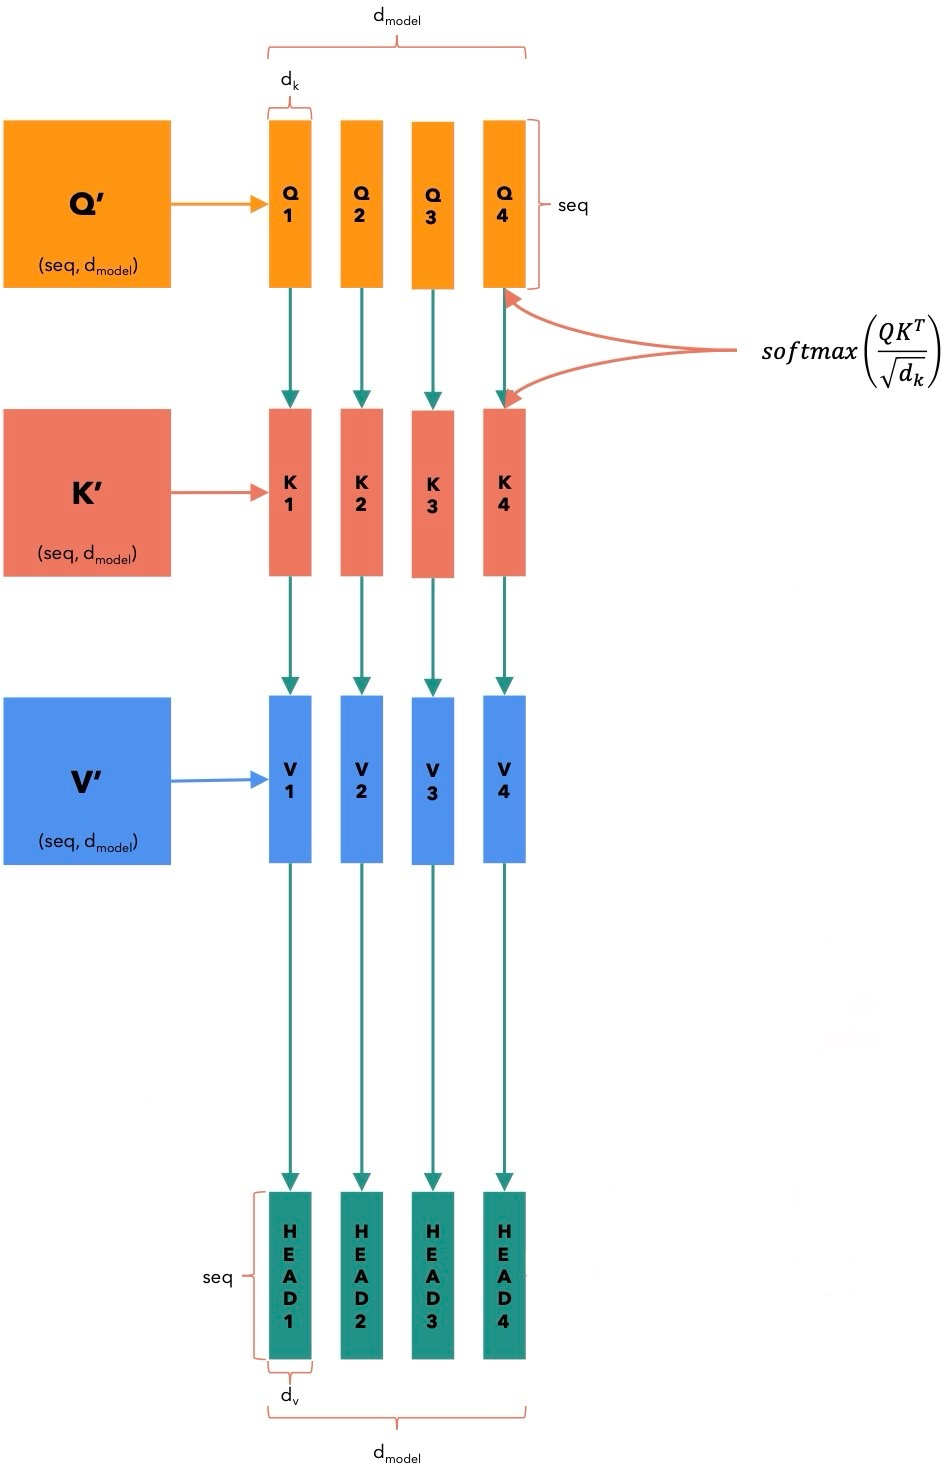
\includegraphics[width=0.8\linewidth]{img/mh-step-2.jpeg}
\caption{\textbf{(Alternative Approach, \textit{Step 2})} In this case, the matrices $Q', K'$, and $V'$, obtained in the previous step, are split into $h$ matrices of size $seq\times d_k$ \cite{git-hub}. Dot-Product Attention is then calculated on each triplet of sub-matrices $(Q_1,K_1,V_1), \dots, (Q_h, K_h, V_h)$. The result of this operation will consist of $h$ head matrices with $head_i \in \mathbb{R}^{seq\times d_v}$.}
\label{fig:mh_step2}
\end{figure}

\paragraph{Concatenation of Head Outputs}
In this phase, the $h$ heads, just computed, are concatenated along axis \textit{1} to produce a single matrix of size $seq\times d_{model}$ \cite{arxiv-attention, stanford}:
\begin{equation}
Concat=[head_1 \oplus head_2 \oplus \dots\oplus head_h] \in \mathbb{R}^{seq\times (h \cdot d_{v})}
\end{equation}

where:
\begin{itemize}
\item $\oplus$ represents concatenation along axis \textit{1} \cite{git-hub}
\end{itemize}
Note how the dimension of the concatenation matrix $Concat$, in this case, is equivalent to $seq\times d_{model}$ \cite{arxiv-attention}:
$$
seq\times (h\cdot d_v) = seq \times \left(h \cdot \frac{d_{model}}{h}\right) = seq \times d_{model}
$$
\begin{figure}[H]
\centering
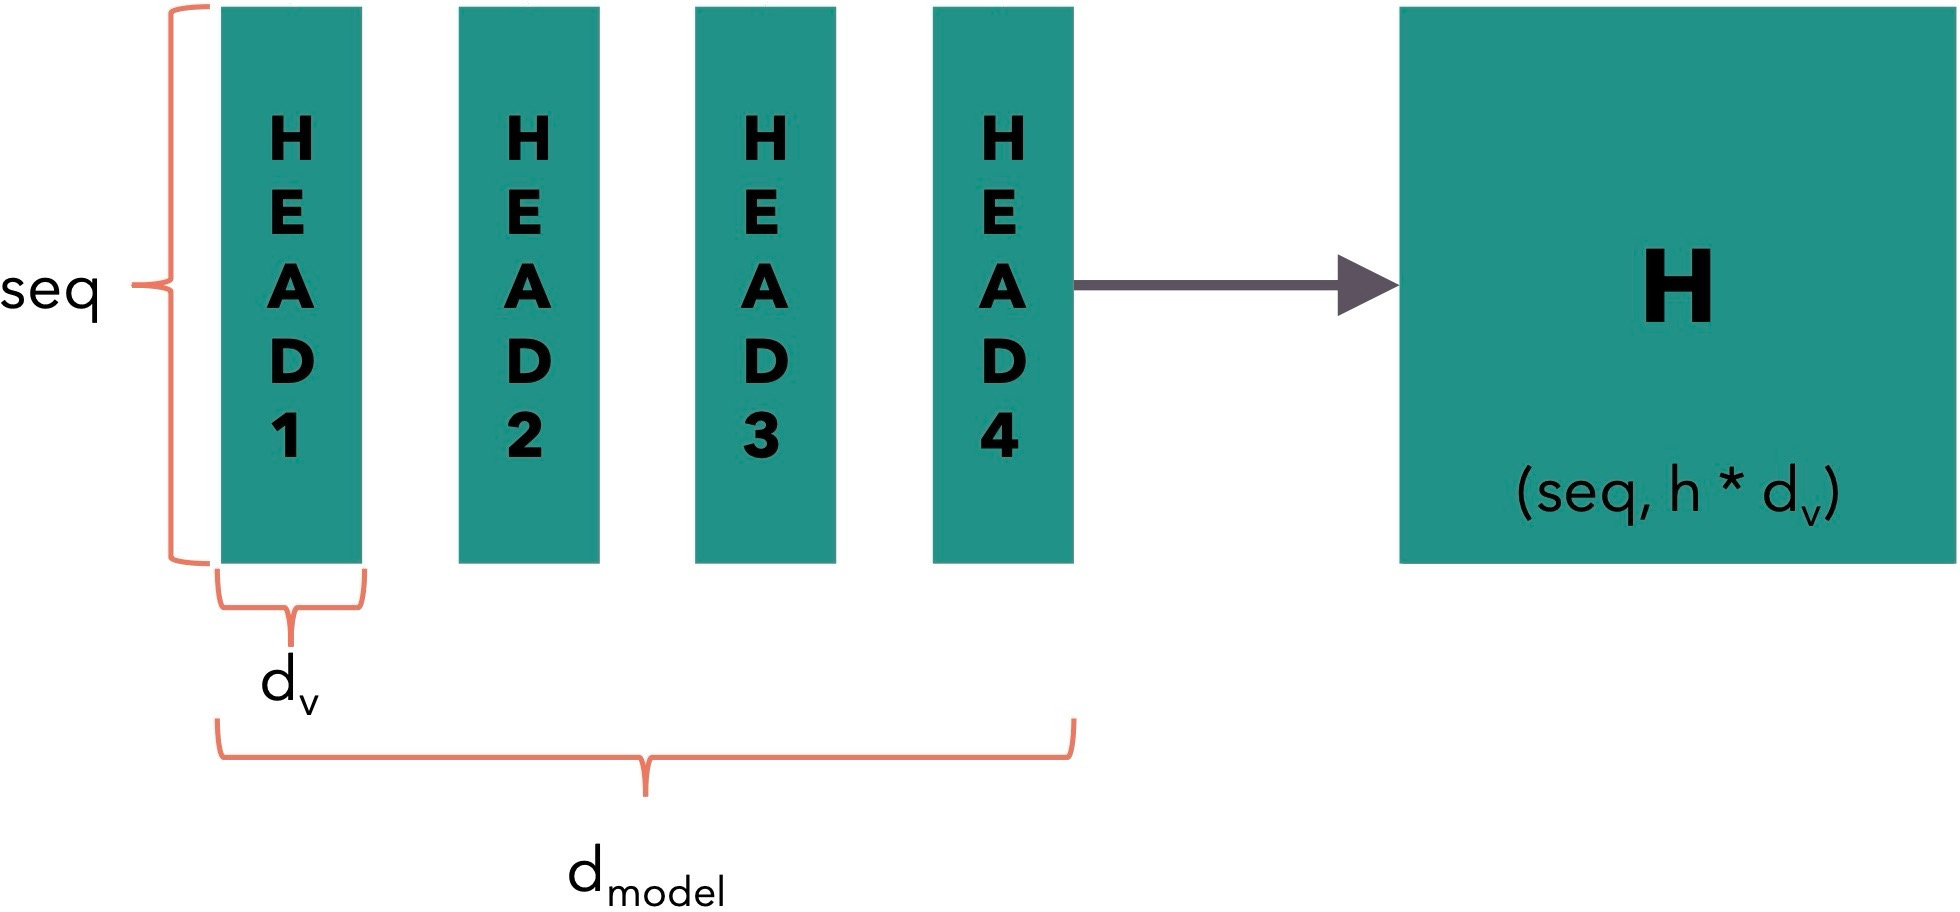
\includegraphics[width=0.55\linewidth]{img/mh-step-3.jpeg}
\caption{\textbf{(Alternative Approach, \textit{Step 3})} The head matrices obtained as a result of Self-Attention are concatenated along axis 1 \cite{git-hub}. The result is a matrix $H$ of dimension ${seq\times (h\cdot d_v)}$.}
\label{fig:mh_step3}
\end{figure}

\paragraph{Final Projection}
Finally, the concatenated output is projected through the final weight matrix $W^O \in \mathbb{R}^{(h\cdot d_v)\times d_{model}}$ \cite{arxiv-attention, stanford}:
$$
MultiHead(Q, K, V)=Concat(head_1, head_2, \dots, head_h)W^O \in \mathbb{R}^{seq\times d_{model}}
$$
Note how, in this case as well (analogously to Self-Attention), the output matrix has the same dimension $seq\times d_{model}$ as the input matrix $X$ \cite{arxiv-attention, git-hub}.

\begin{figure}[H]
\centering
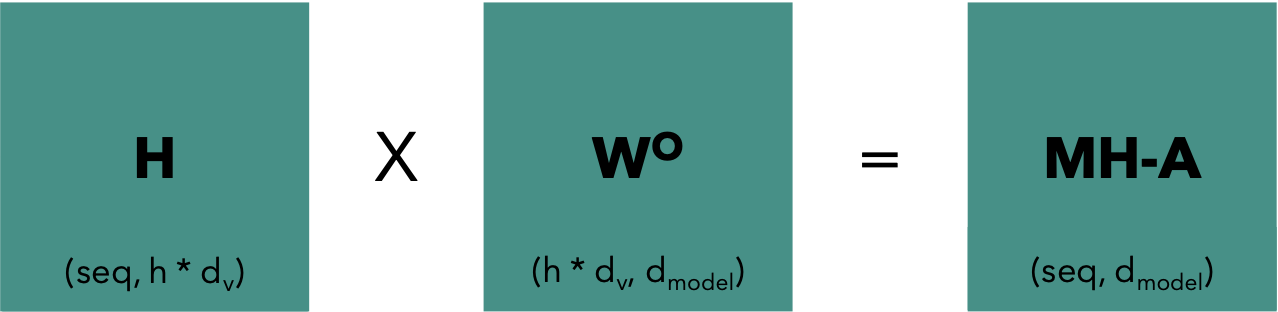
\includegraphics[width=0.65\linewidth]{img/mh-step-4.png}
\caption{\textbf{(Alternative Approach, \textit{Step 4})} The concatenated matrix $H$ is projected onto the output matrix $W^O \in \mathbb{R}^{(h \cdot d_v) \times d_{model}}$, producing the resulting matrix $MH\_A \in \mathbb{R}^{seq \times d_{model}}$ \cite{git-hub}. The matrix $MH\_A$ thus constitutes the result of Multi-Head Attention.}
\label{fig:mh_step}
\end{figure}



%\subsubsection{Layer Normalization e Residual Connections}
%\label{sub:layer_norm_residual_connection}
%\noindent
%Questi componenti sono essenziali per la stabilità numerica e la convergenza durante l'addestramento. Esistono due convenzioni principali: post-LN e pre-LN, con quest'ultima che ha dimostrato maggiore facilità di addestramento.

\subsection{Normalization and Residual Mechanisms}
As shown in Figure \ref{fig:transformer}, applied to each sub-layer of the Transformer (Multi-Head Attention and Feed-Forward Network) is a component called Add \& Norm \cite{arxiv-attention}, which combines two operations:
\begin{itemize}
\item \textbf{Add (Residual Connection):} Takes the output of a sub-layer (Multi-Head Attention or Feed Forward) and adds it to the original input of the same sub-layer \cite{arxiv-attention, arxiv-skipconnection-survey}.
\item \textbf{Norm (Layer Normalization):} Applies a normalization that standardizes the vector values for each token in the sequence \cite{arxiv-attention, stanford}.
\end{itemize}
This component plays a fundamental role in maintaining training stability and enabling the training of deep networks \cite{arxiv-attention, arxiv-skipconnection-survey}.

\subsubsection{Residual Connection (Add)}
A residual connection, or skip connection, is a direct path connecting the input of a sub-layer to its output, bypassing the sub-layer itself \cite{arxiv-attention, arxiv-skipconnection-survey}:
\begin{equation}
Output_{residual} = x + SubLayer(x)
\end{equation}

where:
\begin{itemize}
\item $x$ represents the input of the \textit{SubLayer}
\item $SubLayer(x)$ represents the output of the \textit{SubLayer}
\end{itemize}
The benefits provided by the application of this state are:
\begin{itemize}
\item \textbf{Mitigation of the Vanishing Gradient Problem:} The primary advantage of residual connections is that they allow the gradient to bypass the sub-layer during backpropagation \cite{arxiv-skipconnection-survey}. Formally, the gradient of the loss function $L$ with respect to the input $x$ is:
\begin{equation}
\frac{\partial L}{\partial x} = \frac{\partial L}{\partial Output_{residual}} \frac{\partial Output_{residual}}{\partial x}
\end{equation}

Calculating $\frac{\partial Output_{residual}}{\partial x}$ separately, we obtain:
$$
\frac{\partial Output_{residual}}{\partial x} = \frac{\partial \left(x + SubLayer(x)\right)}{\partial x} = \frac{\partial x}{\partial x} + \frac{\partial SubLayer(x)}{\partial x} = 1 + \frac{\partial SubLayer(x)}{\partial x}
$$
This yields:
$$
 \frac{\partial L}{\partial x} = \frac{\partial L}{\partial Output_{residual}} \left( 1 + \frac{\partial SubLayer(x)}{\partial x} \right)
$$

Note how the term $1$ guarantees the existence of a path with a non-zero gradient, regardless of how small $\frac{\partial SubLayer(x)}{\partial x}$ becomes \cite{arxiv-skipconnection-survey}. This characteristic prevents the vanishing gradient problem, where gradients become exponentially smaller across layers, making the training of deep networks impossible \cite{arxiv-attention, arxiv-skipconnection-survey}.

\item \textbf{Information Preservation:} The residual connection preserves the original information from the input, ensuring that crucial information is not lost within the sub-layer \cite{arxiv-skipconnection-survey}. The sub-layer only adds its contribution, but the original information is always present.

\item \textbf{Depth Stability:} It allows for the training of very deep Transformers without performance degradation at inference time \cite{arxiv-attention, arxiv-skipconnection-survey}. It has been demonstrated that adding more layers without residual connections often worsens performance; with residual connections, adding layers generally improves or maintains performance during inference.
\end{itemize}

\subsubsection{Layer Normalization (Norm)}
Layer Normalization is a technique that normalizes activation values along the feature (embedding) dimension rather than along the batch dimension (as performed in Batch Normalization) \cite{batch_norm}.

\begin{figure}[H]
\centering
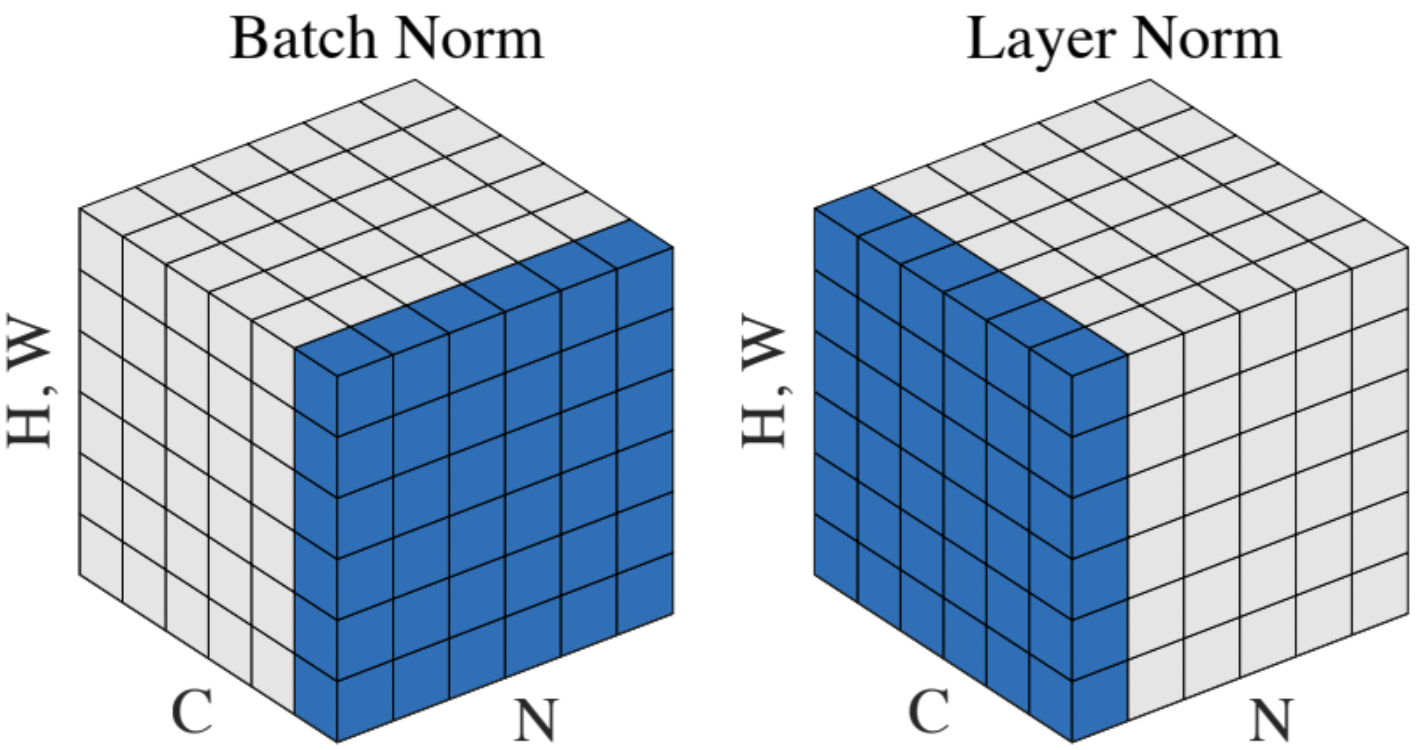
\includegraphics[width=0.5\linewidth]{img/batch_vs_norm.png}
\caption{Graphical representation of the difference between \textbf{Batch Normalization} (left) and \textbf{Layer Normalization} (right) via two 3D tensors with dimensions \textit{N} (batch), \textit{C} (channels/features), \textit{H} (height), and \textit{W} (width) \cite{batch_norm}. The blue region highlights the dimensions along which normalization statistics (mean and variance) are calculated. Note that in \textbf{Batch Norm}, this occurs vertically along \textit{N}, making it dependent on the batch size \cite{batch_norm}; in \textbf{Layer Norm}, it occurs horizontally along C, H, and W (thus independent of the batch) \cite{batch_norm}, which is ideal for variable sequences such as in Transformers.}
\label{fig:batch_vs_layer_norm}
\end{figure}

Formally, for each token $i$ in the sequence, given the activation vector $x_i\in \mathbb{R}^{d_{model}}$, Layer Normalization computes \cite{arxiv-attention, stanford}:
\begin{equation}
LayerNorm(x_i)= \gamma \odot \frac{x_i - \mu}{\sqrt{\sigma^2 + \epsilon}} + \beta
\end{equation}

where:
\begin{itemize}
\item $\mu = \frac{1}{d_{model}} \sum^{d_{model}}_{j=1}x_{ij}$ is the mean of the activations for token $i$ across all its components
\item $\sigma^2_i=\frac{1}{d_{model}}\sum^{d_{model}}_{j=1} (x_{ij}-\mu_i)^2 $ is the variance
\item $\epsilon$ is a very small constant ($\approx 10^{-6}$) added for numerical stability
\item $\gamma \in \mathbb{R}^{d_{model}}$ is the learned \textit{scaling vector}
\item $\beta \in \mathbb{R}^{d_{model}}$ is the learned \textit{shift vector}
\item $\odot$ represents the element-wise product
\end{itemize}
The benefits provided by Layer Normalization are:
\begin{itemize}
\item \textbf{Gradient Stability:} Layer normalization maintains the scale of activations within a reasonable range (typically mean 0 and variance 1 after normalization), helping to prevent gradients from becoming too large (\textit{exploding gradients}) or too small (\textit{vanishing gradients}) \cite{arxiv-attention, stanford}.

\item \textbf{Mitigation of Internal Covariate Shift:} During training, the distribution of activations in each layer changes continuously (\textit{internal covariate shift}). This slows down training and requires smaller learning rates. Layer normalization reduces this effect \cite{arxiv-attention, stanford}.

\item \textbf{Improved Gradient Flow in Attention:} Input normalization enables the attention mechanism to operate on values with predictable scales \cite{arxiv-attention}. Without normalization, the dot products used in attention calculation could become very large, leading to "explosive" softmax values (close to 0 or 1) and consequently causing gradients to be dangerously close to zero \cite{arxiv-attention, stanford, GeeksForGeeks}.
\end{itemize}

\subsubsection{Configurations: Post-LN vs Pre-LN}
There are two common configurations for the Add \& Norm component in the Transformer \cite{git-hub, stanford}:
\begin{itemize}
\item \textbf{Post-LN} (Post-Normalization)
\item \textbf{Pre-LN} (Pre-Normalization)
\end{itemize}
In the original paper \textit{"Attention Is All You Need"}, the \textbf{Post-LN} configuration is used \cite{arxiv-attention}:
\begin{equation}
Output = LayerNorm(X + SubLayer(X))
\end{equation}

where:
\begin{itemize}
\item $X \in \mathbb{R}^{seq \times d_{model}}$ represents the input matrix of the \textit{sublayer}
\end{itemize}
In this manner, the residual is added first, and the normalization is applied only subsequently \cite{arxiv-attention, git-hub}.
This approach can ensure more stable training in some cases. Generally, however, the Post-LN configuration requires a learning rate \textit{warmup} phase to manage high-magnitude gradients close to the output layer \cite{arxiv-attention, stanford}.

In the \textbf{Pre-LN} configuration, used in modern models like \textit{GPT} and newer \textit{BERT} variants, \footnote{It is worth noting that while the original implementation of BERT used a Post-LN configuration\cite{xiong2020ln}, subsequent analyses and modern variants (and virtually all recent Large Language Models) have adopted Pre-LN or alternative normalizations (like RMSNorm)\cite{liu2023b2t,xiong2020ln} to improve training stability at greater depths\cite{liu2023b2t}.} we have:
\begin{equation}
Output = X + SubLayer(LayerNorm(X))
\end{equation}

Essentially, the input is first normalized, then passed to the sub-layer, and only finally is the residual connection added \cite{git-hub}.
The Pre-LN approach guarantees:
\begin{itemize}
\item High training stability without requiring learning rate \textit{warmup} \cite{git-hub, stanford}
\item Better gradients through the residual layers \cite{arxiv-skipconnection-survey, attention-is-not}
\item Higher learning rates \cite{git-hub, stanford}
\end{itemize}


\subsection{Position-wise Feed-Forward Networks}
The feed-forward layer (FFN), also referred to as the position-wise feed-forward network, is a fundamental component of the Transformer architecture \cite{arxiv-attention, attention-is-not} that accompanies the multi-head attention mechanism \cite{arxiv-attention}. This layer consists of a fully connected neural network \cite{arxiv-attention, stanford} that applies the same non-linear transformations to each token in the sequence, independently \cite{arxiv-attention, stanford, GeeksForGeeks}. In this manner, non-linearity is introduced into the Transformer architecture, which, consequently, becomes capable of learning complex non-linear relationships \cite{stanford, attention-is-not}.

The feed-forward layer is composed of two \textbf{linear} layers separated by a \textbf{non-linear} activation function \cite{arxiv-attention}. The structure can be represented as:
\begin{equation}
FFN(x)=\phi(x_iW_1 + b_1)W_2+b_2
\end{equation}

where:
\begin{itemize}
\item $x_i \in \mathbb{R}^{d_{model}}$ represents a single token with $i=\{1,\dots, seq\}$
\item $W_1 \in \mathbb{R}^{d_{model}\times(4\cdot d_{model})}, W_2 \in \mathbb{R}^{(4 \cdot d_{model})\times d_{model}}$ represent the weight matrices
\item $b_1 \in \mathbb{R}^{4\cdot d_{model}}, b_2\in \mathbb{R}^{d_{model}}$ represent the bias vectors
\item $\phi$ represents the activation function (obviously non-linear)
\end{itemize}

In the original Transformer, the activation function $\phi$ is a simple $ReLU(x)$ \cite{arxiv-attention}, but in more modern implementations, it is often implemented as $GELU$ or $SwiGLU$ \cite{stanford, attention-is-not}. \footnote{Unlike ReLU, which outputs strictly zero for negative inputs (potentially causing the 'dying ReLU' problem), functions like GELU (Gaussian Error Linear Unit) are smooth and non-monotonic \cite{stanford}. This allows for better gradient flow and has been empirically shown to improve convergence in deep Transformer models (e.g., BERT, GPT-3) \cite{stanford, attention-is-not}.}
%\begin{center}
%\begin{tikzpicture}[
 % node distance=1cm and 1.5cm,
%layer/.style={rectangle, draw, minimum width=2.5cm, minimum height=1cm, align=center},
 % arrow/.style={-Straight Barb, thick}
%]

% Nodi del diagramma
%\node (input_arrow) {$x_i$}; % Punto di partenza per la freccia di input
%\node (linear1) [layer, below=of input_arrow] {Linear};
%\node (relu)[layer, below=of linear1] {ReLU};
%\node (linear2) [layer, below=of relu]{Linear};
%\node (output_arrow) [below=of linear2] {$FFN(x_i)$}; % Punto di arrivo

% Frecce che collegano i layer
%\draw[arrow] (input_arrow) -- (linear1);
%\draw[arrow] (linear1) -- (relu);
%\draw[arrow] (relu)-- (linear2);
%\draw[arrow] (linear2) -- (output_arrow);

%\end{tikzpicture}
%\end{center}


\begin{figure}[H]
\centering
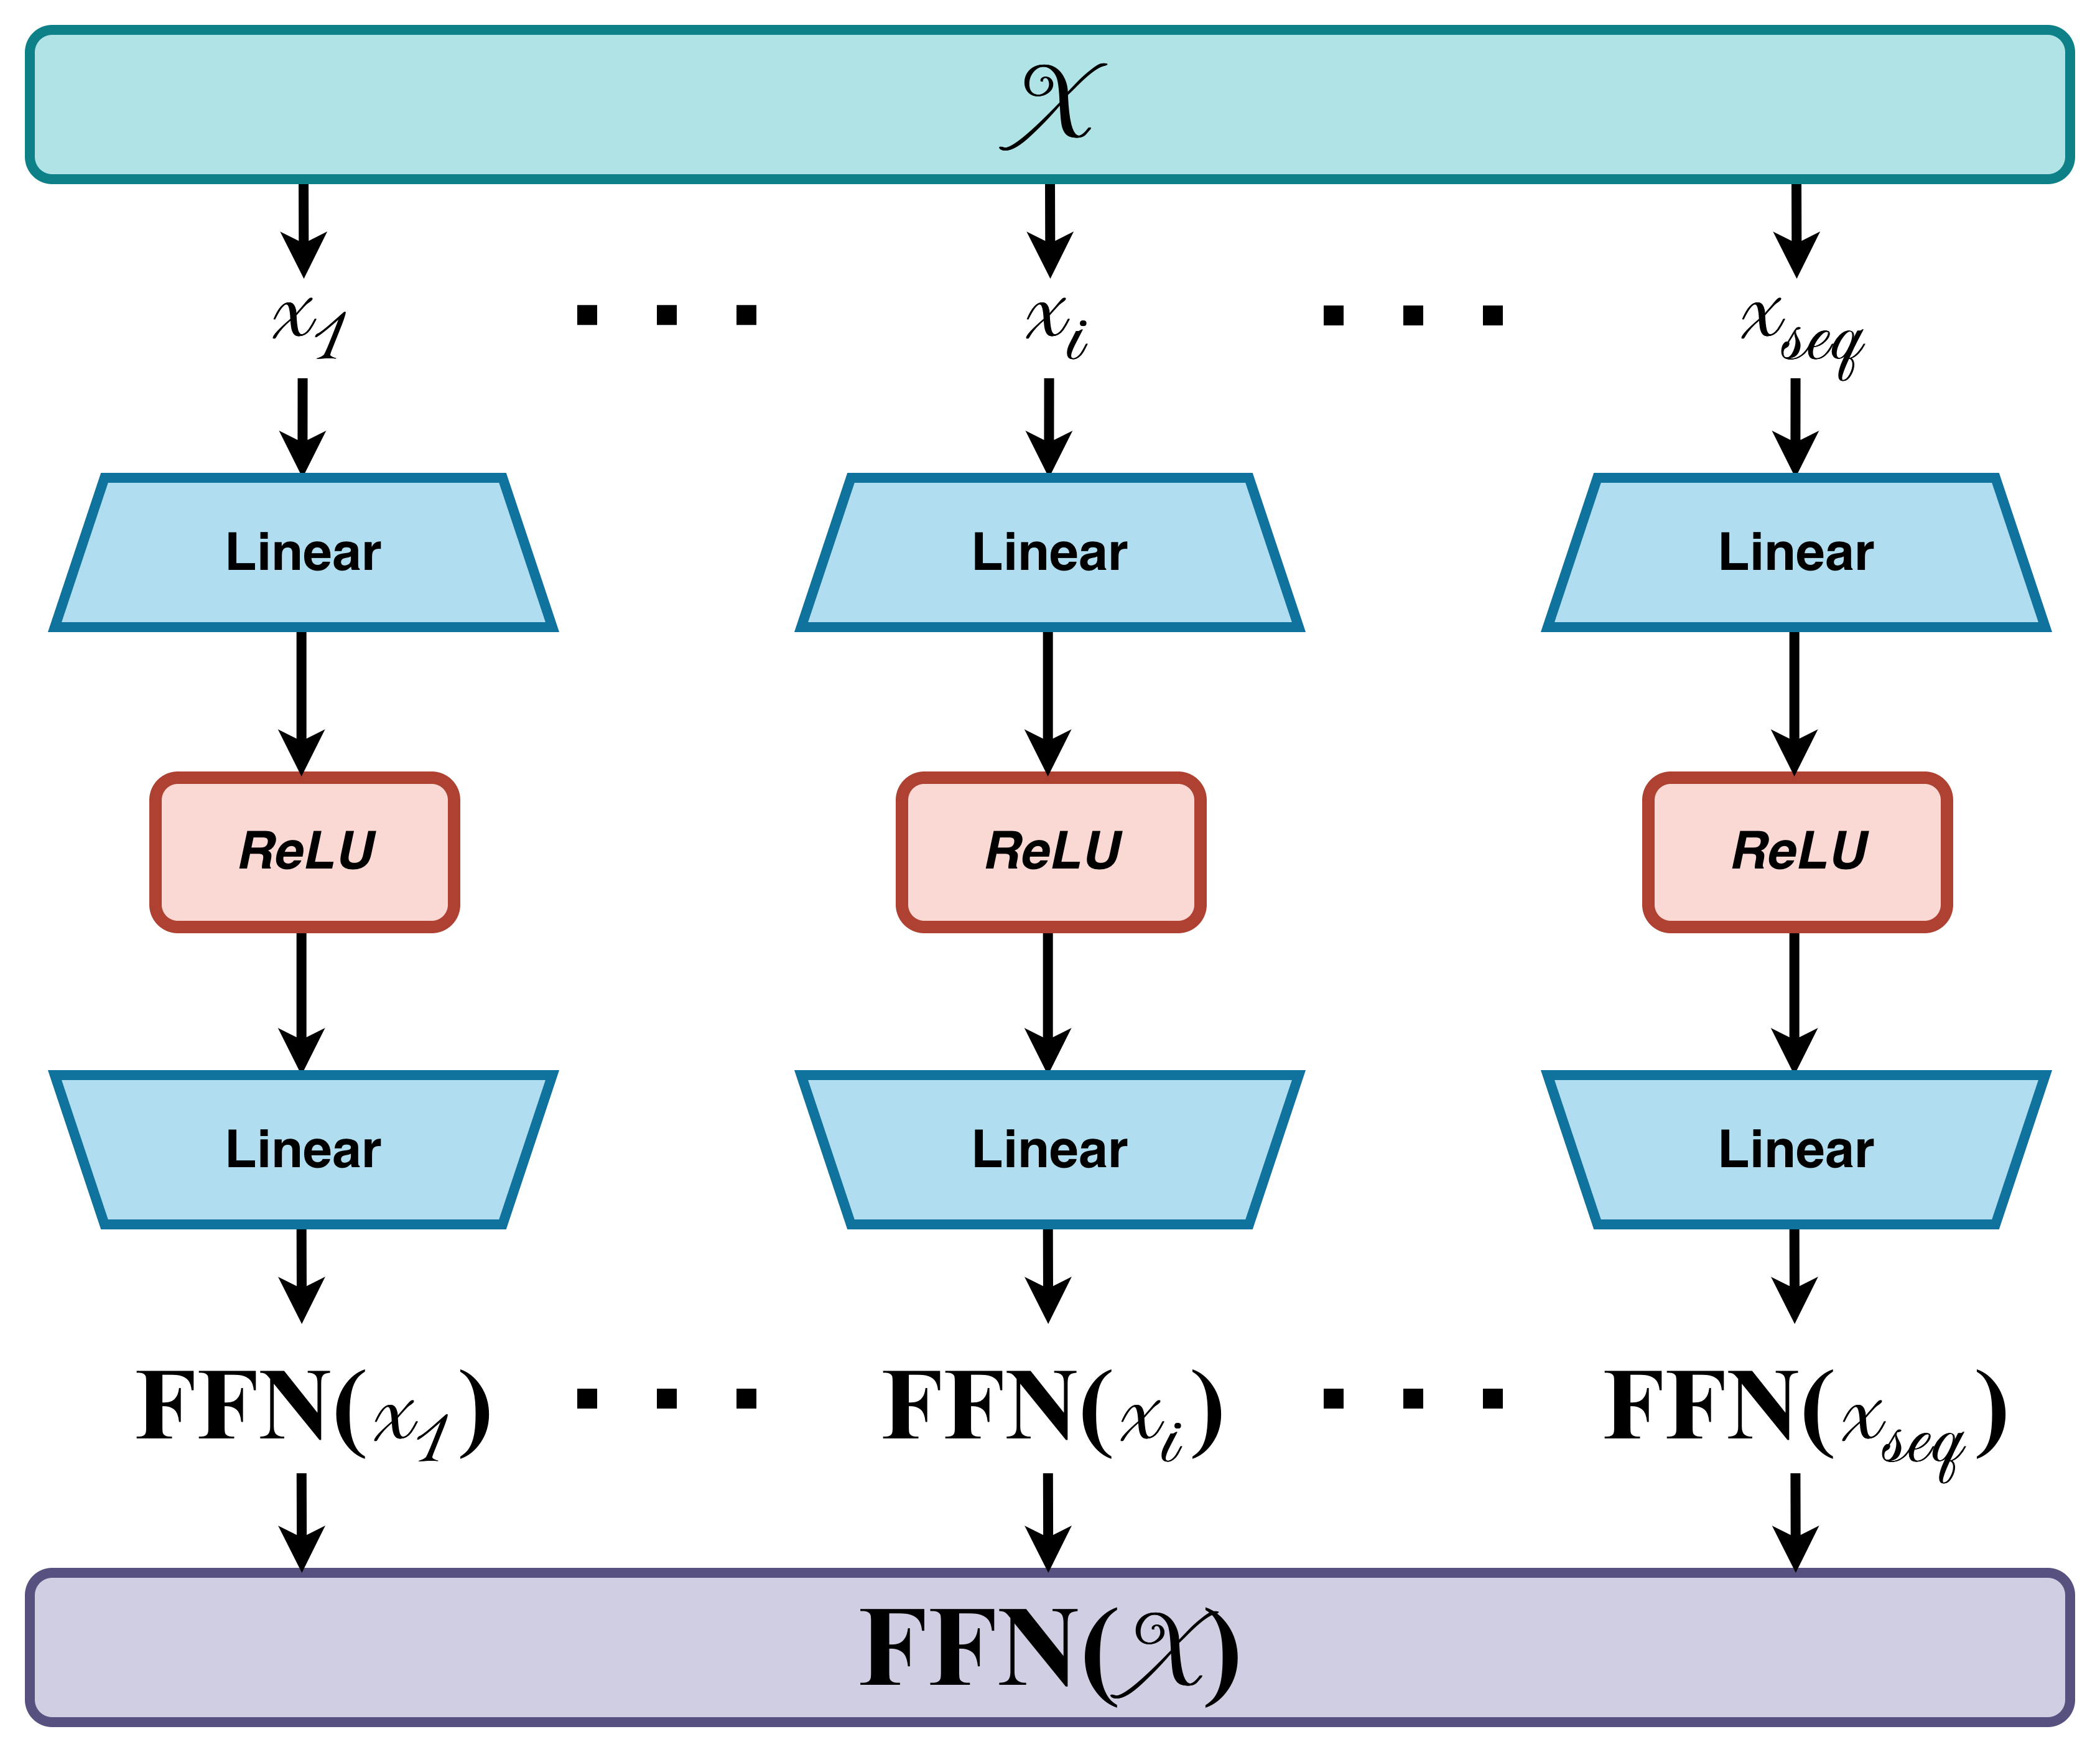
\includegraphics[width=0.5\linewidth]{img/ffn_3.png}
\caption{Schematic representation of the feed-forward network. The operations are shown in sequence: linear transformation (expanding the dimensionality), application of the ReLU activation function, and a second linear transformation (projecting back to the original dimensionality).}
\label{fig:ffn}
\end{figure}
The feed-forward layer thus complements the attention mechanism \cite{attention-is-not}; indeed, while attention mixes and weighs information originating from different tokens in the sequence (in a linear manner), the FFN applies further processing to each token individually, enabling the model to capture complex and non-linear patterns \cite{attention-is-not}.

\subsection{Encoder-Decoder: Integration of the Transformer Architecture}
Up to this point, the components of the Transformer architecture have been examined individually: tokenization, the self-attention mechanism, multi-head attention, residual connections, layer normalization, and the feed-forward network. Each of these elements plays a specific role in information processing. The aim of this section is to integrate all this knowledge to understand how the encoder and decoder work together, forming an architecture capable of transforming an input sequence into a plausible output sequence while maintaining semantic context and long-range relationships.

\subsubsection{Encoder}
The encoder consists of $N$ identical layers stacked sequentially (in the original paper, $N=6$ is used) \cite{arxiv-attention}.
Each encoder layer contains two sub-layers \cite{arxiv-attention, stanford}:
\begin{enumerate}
\item \textbf{Multi-Head Self-Attention:} Allows the tokens of the initial sequence to relate to one another \cite{arxiv-attention, GeeksForGeeks}.
\item \textbf{Position-wise Feed-Forward Network:} Applies non-linear transformations to each token independently, enabling the model to learn complex non-linear relationships \cite{arxiv-attention, attention-is-not}.
\end{enumerate}
Each of these two sub-layers is then followed (or preceded) by an Add \& Norm component, which applies a skip connection and layer normalization \cite{arxiv-attention, git-hub}.

The output of the final encoder layer $N$ consists of an output matrix $E^{(N)} \in \mathbb{R}^{seq \times d_{model}}$, representing a contextualized embedding of each token in the input sequence, enriched with information coming from all other tokens in the sequence via the self-attention mechanisms \cite{arxiv-attention, stanford, hashnode}.
\begin{figure}[H]
\centering
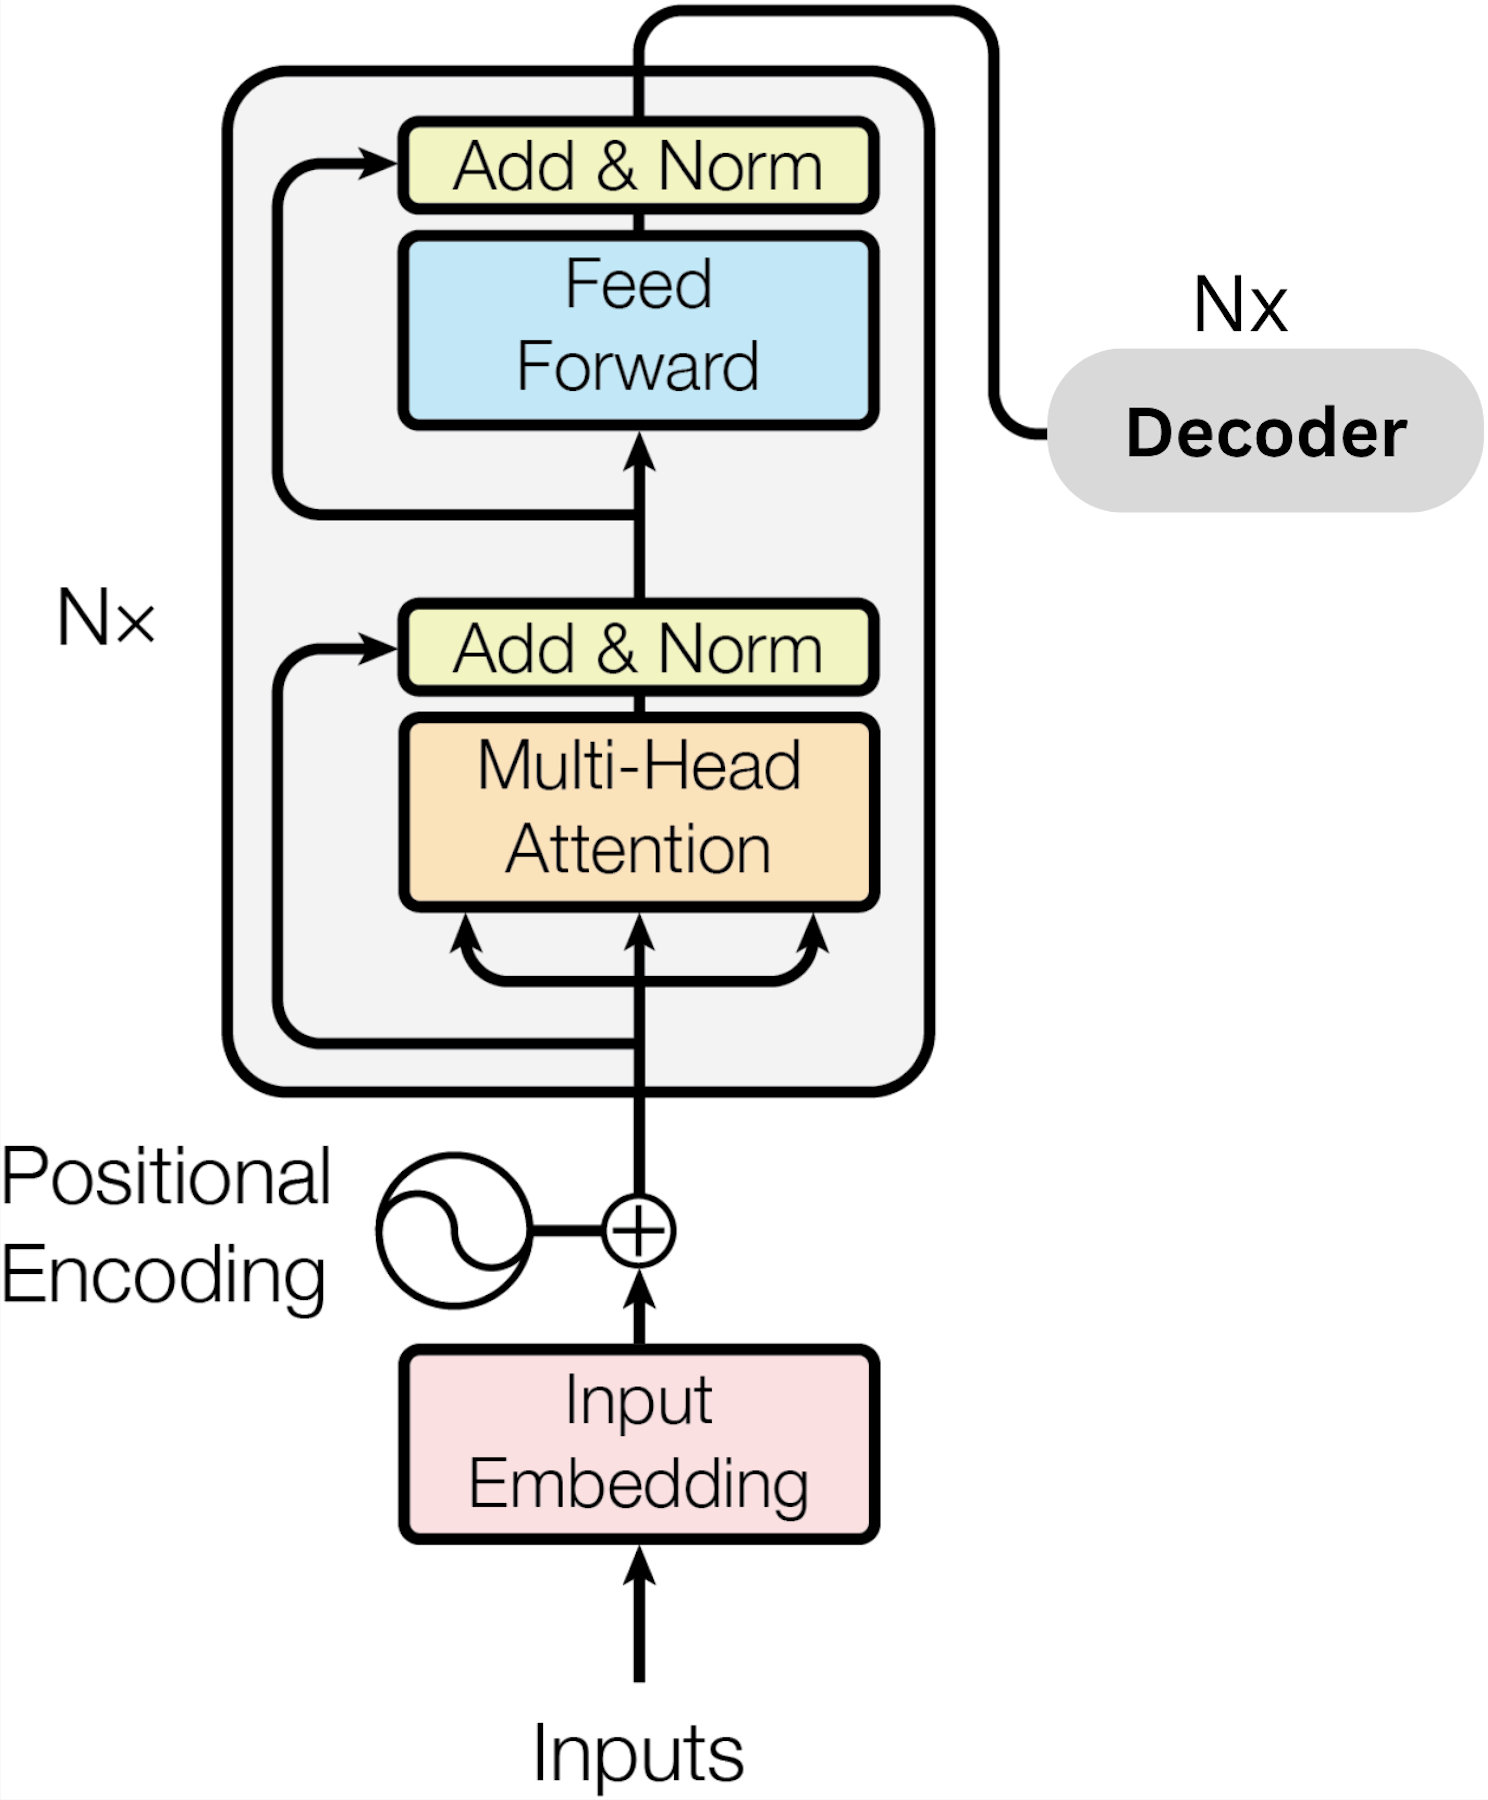
\includegraphics[width=0.5\linewidth]{img/encoder-schema_3.png}
\caption{Schematic representation of the flow followed by the input sequence within the $N$ encoder layers. The output matrix $E^{(N)} \in \mathbb{R}^{seq \times d_{model}}$ is sent to the Decoder \cite{arxiv-attention}.}
\label{fig:encoder_schema}
\end{figure}
The properties of the encoder include:
\begin{itemize}
\item \textbf{Breaking of Permutation Equivariance:} Due to positional encoding, the encoder does not possess the property of permutation equivariance; the sequence order is thus explicitly represented \cite{arxiv-attention, Muhammad_Faizan}.

\item \textbf{Full Context Access:} Each token has access to all other tokens in the sequence, allowing for the capture of global dependencies \cite{arxiv-attention, stanford, GeeksForGeeks}.

\item \textbf{Total Parallelization:} All tokens can be processed simultaneously, making the encoder computationally efficient on \textit{GPUs} \cite{arxiv-attention}.
\end{itemize}

\subsubsection{Decoder}
The decoder features a structure similar to that of the encoder; however, it is divided into three sub-layers \cite{arxiv-attention, stanford}:
\begin{enumerate}
\item \textbf{Masked Multi-Head Self-Attention:} Self-attention on a masked version of the output sequence \cite{arxiv-attention, GeeksForGeeks}.
\item \textbf{Multi-Head Cross-Attention:} Attention between the decoder tokens and the encoder representation \cite{arxiv-attention, hashnode}.
\item \textbf{Position-wise Feed-Forward Network:} Analogous to the encoder sub-layer \cite{arxiv-attention, attention-is-not}.
\end{enumerate}
In this case as well, each sub-layer is followed (or preceded) by an Add \& Norm component that applies a skip connection and layer normalization \cite{arxiv-attention, git-hub}.
The decoder, analogous to the encoder, consists of $m=\{1, 2, \dots, N\}$ layers \cite{arxiv-attention}.
\begin{figure}[H]
\centering
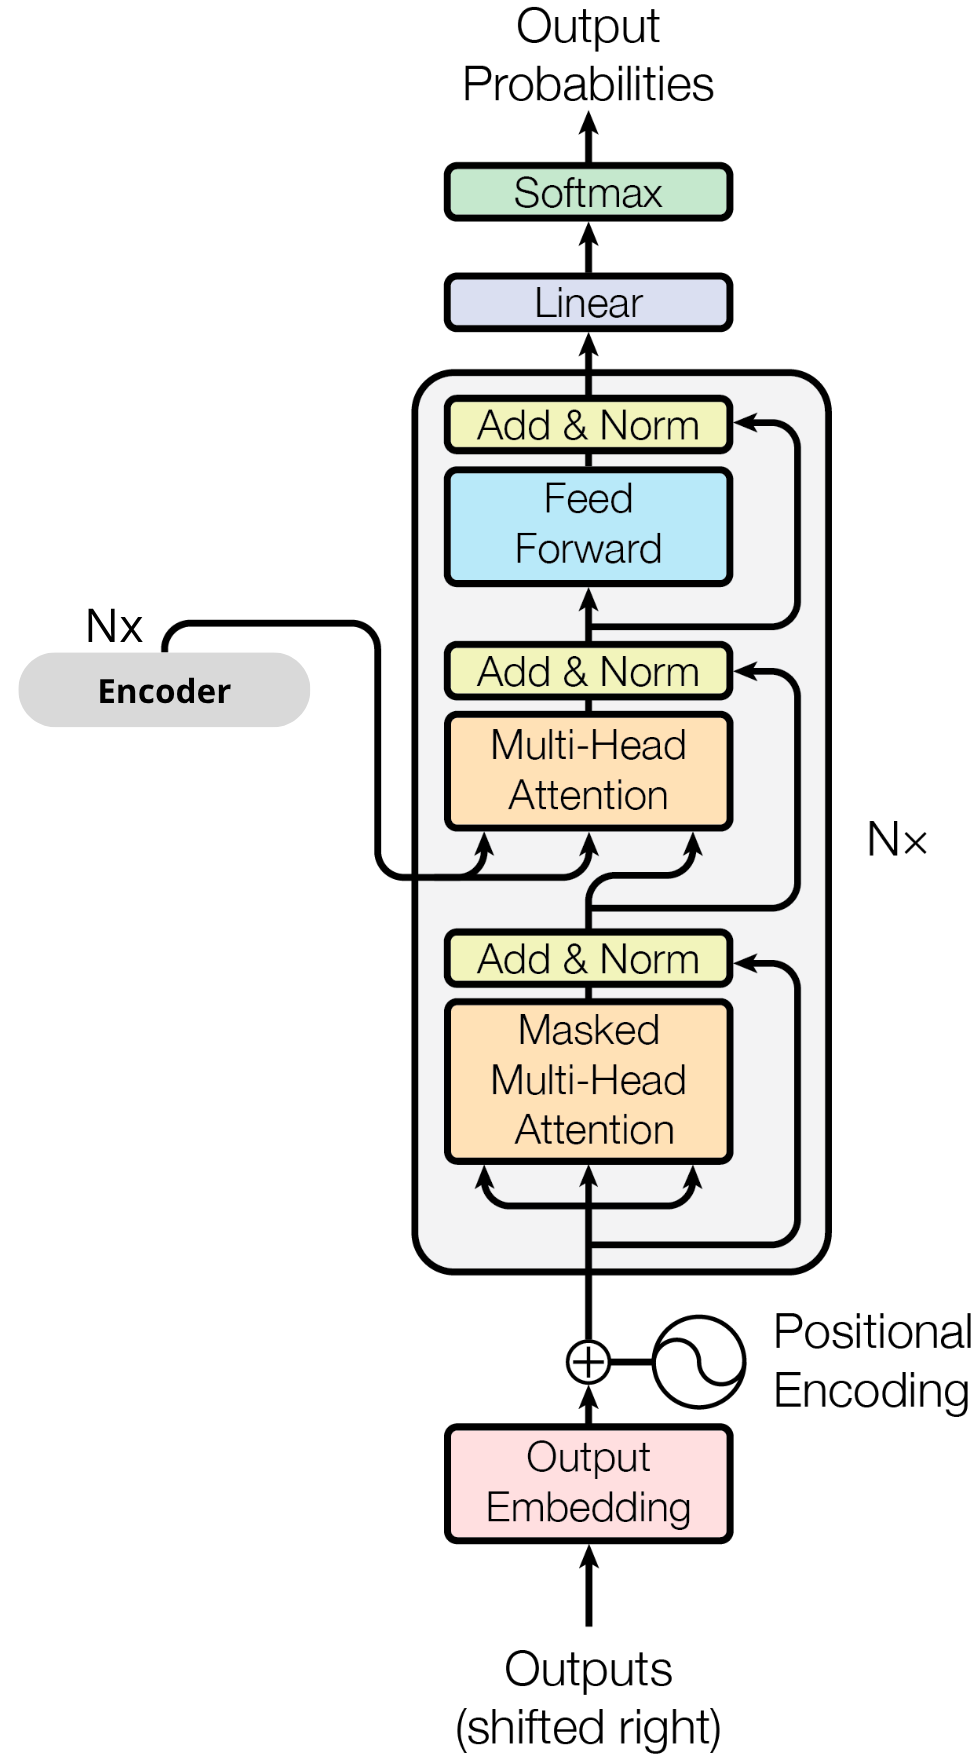
\includegraphics[width=0.5\linewidth]{img/decoder-schema_2.png}
\caption{Schematic representation of the flow followed by the input sequence within the $N$ decoder layers \cite{arxiv-attention}.}
\label{fig:schema}
\end{figure}
The various internal phases of the decoder are described below:

\paragraph{Masked Self-Attention}
The crucial difference compared to the encoder lies in the decoder's self-attention mechanism \cite{arxiv-attention}. During training, the model must generate output individually for each token $x_i$, without access to future tokens ($x_{i+1}, x_{i+2}, \dots$) \cite{arxiv-attention, stanford}. For this reason, a "mask" is applied to the attention matrix \cite{arxiv-attention, GeeksForGeeks}.



During the calculation of the $Attention$ matrix, before applying the $softmax$, a very large negative value (typically $-\infty$) is added to future positions \cite{arxiv-attention, hashnode}.\footnote{This training strategy, where the model is fed the actual ground-truth tokens from the previous steps rather than its own generated predictions, is formally known as \textit{Teacher Forcing} \cite{stanford}. It enables parallelization during training, unlike the sequential generation required during inference.} A mask matrix $M\in \mathbb{R}^{seq\times seq}$ is therefore added:
\begin{equation}
Attention(Q_i,K_i,V_i) = softmax\left( \frac{QK^T}{\sqrt{d_k}} + M\right)V
\end{equation}

The mask matrix is defined for each token $x_i$ as:
$$
M=
\begin{cases}
\quad 0 \quad \quad \textit{ if}\quad i \ge j \\
-\infty \quad \quad \textit{if} \quad i < j
\end{cases}
$$
where:
\begin{itemize}
\item $i$ indicates the rows of $M$
\item $j$ indicates the columns of $M$
\end{itemize}
The mask matrix will therefore be of the form:
%%%%%% MATRICE NELL'ALTRA FORMA, SCEGLI QUALE USARE.
%$$
 % M = 
%\begin{bmatrix}
%0 & -\infty & -\infty & \cdots & -\infty \\
%0 & 0 & -\infty & \cdots & -\infty \\
%0 & 0 & 0 & \cdots & -\infty \\
%\vdots & \vdots & \vdots & \ddots & \vdots \\
%0 & 0 & 0 & \cdots & 0
%\end{bmatrix}_{seq \times seq}
%$$
$$
M = 
\begin{pmatrix}
0 & -\infty & -\infty & -\infty & \cdots & -\infty \\
0 & 0 & -\infty & -\infty & \cdots & -\infty \\
0 & 0 & 0 & -\infty & \cdots & -\infty \\
\vdots & \vdots & \vdots & \vdots & \ddots & \vdots \\
\vdots & \vdots & \vdots & \vdots & \ddots & \vdots \\
0 & 0 & 0 & \cdots & \cdots & 0
\end{pmatrix}_{seq \times seq}
$$
This configuration ensures that the calculation of the $softmax$, in positions $j > i$, returns a probability value of $0$ for future tokens.
\begin{figure}[H]
\centering
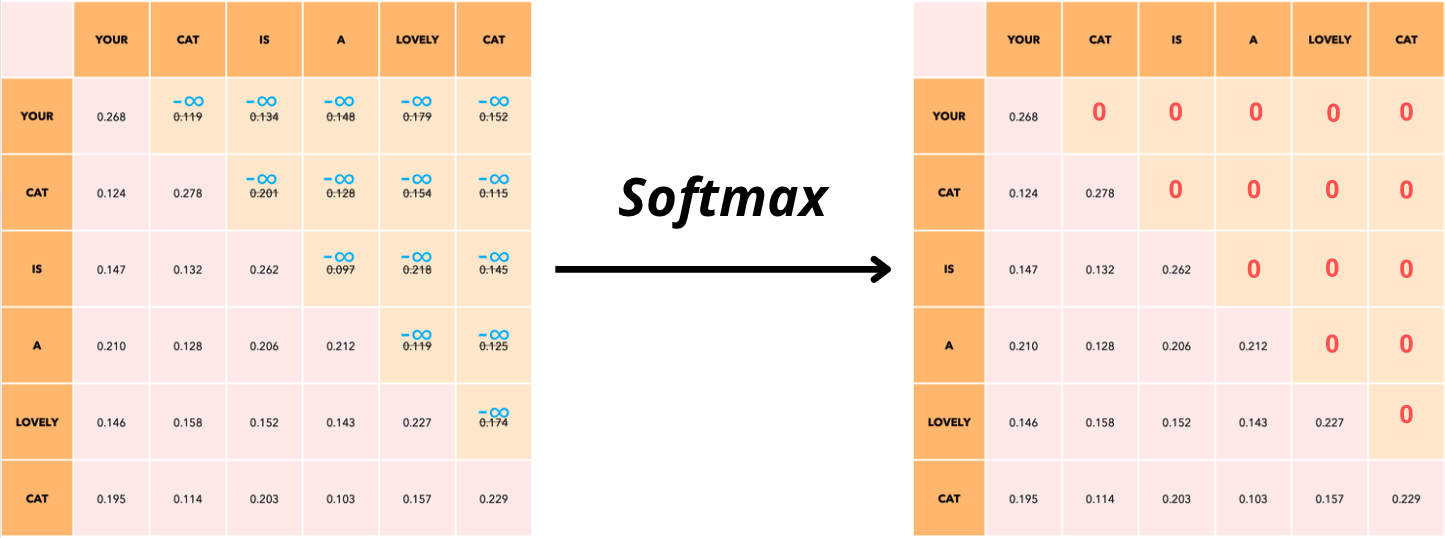
\includegraphics[width=1\linewidth]{img/masked_process.png}
\caption{Example of applying the mask matrix $M\in \mathbb{R}^{seq\times seq}$ to the matrix $\frac{QK^T}{\sqrt{d_k}}$ (left) and the subsequent application of the $softmax$ function \cite{git-hub}. The resulting $AttentionWeights$ matrix (right) presents a score of $0$ on every $token_j$ where $j>i$.}
\label{fig:masked_process}
\end{figure}

\paragraph{Cross-Attention} The second sub-layer of the decoder introduces the cross-attention mechanism \cite{arxiv-attention}. Unlike self-attention, in this case:
\begin{itemize}
\item The Query matrix $Q \in \mathbb{R}^{seq_{out} \times d_k}$ originates from the decoder output sequence of the previous layer \cite{arxiv-attention, hashnode}.
\item The Key matrix $K\in \mathbb{R}^{seq \times d_k}$ and the Value matrix $V \in \mathbb{R}^{seq \times d_v}$ originate from the encoder representation \cite{arxiv-attention, stanford}.
\end{itemize}
Formally:
$$
CrossAttention^{(m)} = MultiHeadAttention(Q_{decoder^{(m-1)}}, K_{encoder}, V_{encoder})
$$
where:
\begin{itemize}
\item $Q_{decoder^{(m-1)}} \in \mathbb{R}^{seq_{out}^{(m-1)} \times d_k}$ represents the query from the previous decoder layer $m-1$.
\end{itemize}
The Cross-Attention mechanism thus allows the model, using the Query matrix, to search for and extract information from the Key and Value matrices \cite{hashnode, stanford}.

\paragraph{Generation of the Final Output Matrix}
According to the architecture described in \textit{"Attention Is All You Need"} \cite{arxiv-attention}, following each Cross-Attention phase, the resulting matrix $CrossAttention^{(m)}$ passes through:
\begin{enumerate}
\item \textbf{Residual Connection + Layer Normalization} \cite{arxiv-attention, arxiv-skipconnection-survey}
\item \textbf{Position-wise Feed-Forward Network} \cite{arxiv-attention, attention-is-not}
\item \textbf{Residual Connection + Layer Normalization} \cite{arxiv-attention, git-hub}
\end{enumerate}
The output of the decoder after $N$ layers is a representation $D^{(N)}\in \mathbb{R}^{seq_{out} \times d_{model}}$ \cite{arxiv-attention}, where each row represents an output token contextualized with respect to both the other output tokens and the entire input sequence \cite{stanford, hashnode}.

\subsubsection{Output Projection and Probability Distribution}
After passing through all $N$ encoder and decoder layers, the final sequence representation $D^{(N)}$ must be transformed into a probability distribution over the vocabulary $V$ \cite{arxiv-attention, stanford}.

The probability distribution over the vocabulary is produced in two phases \cite{arxiv-attention}:



\paragraph{Linear Layer} The representation matrix $D^{(N)}\in \mathbb{R}^{seq_{out} \times d_{model}}$ is projected onto a space with a dimension equal to the vocabulary size $|V|$ \cite{arxiv-attention, git-hub}. This operation produces the logits matrix $L \in \mathbb{R}^{seq_{out} \times |V|}$:
\begin{equation}
L = D^{(N)} W_{output} + b_{output}
\end{equation}

where:
\begin{itemize}
\item $W_{output} \in \mathbb{R}^{d_{model} \times |V|}$ represents the final output weight matrix
\item $b_{output}$ represents the final output bias vector
\end{itemize}

\paragraph{Softmax} The logits, represented by matrix $L$, are finally normalized via the softmax function to obtain the probability matrix $P \in \mathbb{R}^{seq_{out}\times |V|}$ for each output token \cite{arxiv-attention, stanford}. Each row $i$ of matrix $P$ represents a probability distribution over the vocabulary for the token at the $i$-th position of the output sequence \cite{stanford, GeeksForGeeks}.

Formally:
\begin{equation}
P_i = softmax(L_i) \quad \forall i \in \{1,2,\dots,seq_{out}\}
\end{equation}

where:
\begin{itemize}
\item $L_i \in \mathbb{R}^{|V|}$ represents the $i$-th row of $L$
\item $P_{i} \in \mathbb{R}^{|V|}$ represents the $i$-th row of $P$
\end{itemize}
Each element $P_{i,j}$ thus represents the probability predicted by the model that the token at position $i$ of the output sequence corresponds to the $j$-th token of the vocabulary \cite{arxiv-attention, hashnode}.

%%%%%%%%%%%%%%%%%%%%%%%%%%%%%%%%%%%%%%%%%%%%%%
% Capitolo 2 %
%%%%%%%%%%%%%%%%%%%%%%%%%%%%%%%%%%%%%%%%%%%%%%